\documentclass[a4paper,11pt]{report}
%\usepackage{hyperref}
\usepackage{setspace}
\usepackage{url,natbib,amssymb,hyperref,graphicx,wrapfig,setspace,multirow,booktabs,subfig,array,wrapfig,calc}
\usepackage{array}
\newcolumntype{P}[1]{>{\centering\arraybackslash}p{#1}}
\usepackage{fancyhdr}
\usepackage{color}
\usepackage{booktabs,caption,fixltx2e}
\usepackage[round]{natbib}      % References with names and years
%[round]
\usepackage{xr}                 % reference anothe chapter
%\externaldocument[2-]{../CHAPTER2/ch2_LSM_v11}
%\externaldocument[3-]{../CHAPTER3/ch3_sensitivity_v10}
\usepackage{graphicx}
\usepackage{caption}
\usepackage{appendix}
%\usepackage{subfigure}
\usepackage{float}
\usepackage{subfig}
\usepackage{float}
\usepackage{paralist}                % inline lists
\usepackage{gensymb}    % degrees celsius as {\celsius}
%\usepackage{textcomp]    % arrows
\newcommand{\tildetext}{\raise.17ex\hbox{$\scriptstyle\mattt{\sim}$}}
\usepackage{rotating}   %rotate table
%\renewcommand{\arraystretch}{1.5}  %increase space between rows in tables (default is 1) because there is already baselinestrech 1.5 tables become too separated, maybe with normal spacing this command should be used
\usepackage{rotating,booktabs}
\usepackage{threeparttable}
\usepackage{multirow}
\usepackage{color}% color the text
\usepackage{amsmath}
\usepackage{textcomp}
\usepackage{lscape}
% Page setup from thesis template
\topmargin=-10mm
\textwidth=150mm
\textheight=234mm
\headsep=12mm
\oddsidemargin=14mm
%\oddsidemargin=12mm
\evensidemargin=-1mm
%\evensidemargin=1mm
\parindent=6mm
\parskip=1em 

\newlength{\rulewidth}
\setlength{\rulewidth}{150mm} % change to 150mm for printing on
			      % gordon, 149 otherwise???
% 1.5 line spacing so my supervisor can scrawl all over it
\renewcommand{\baselinestretch}{1.50}

\pagestyle{headings}    % chapter number on top

\setcounter{secnumdepth}{4}              %Numbers subsubsections, and lower.
\setcounter{tocdepth}{4}                 %Sets depth of table of contents to include subsubsections.

\pagestyle{fancy}
\fancyhf{}
%\rhead{\fancyplain{}{\textit{\nouppercase\rightmark}}}
\fancyhead[L]{Chapter 6. The impact of vegetation architecture on global photosynthesis limiting regimes}
\fancyfoot[C]{ \thepage\ }

%opening
\title{}
\author{Renato Kerches Braghiere \\ This document was written in \LaTeX \\ Number of words: 12213}
\date{\today}

\begin{document}
\maketitle
\setcounter{chapter}{5} %so next one is 4

\chapter{The impact of vegetation architecture on global photosynthesis limiting regimes}

\section{Introduction}\label{introduction}

In the literature review there is a previous discussion about how three meteorological factors (radiation, temperature, and water) limit photosynthesis, however as already discussed, LSMs treat limiting regimes of photosynthesis based on the Farquhar model \citep{Farquhar1980}, which assumes photosynthesis is given by the co-limitation of three regimes: carbon, light, and electron transport. So, the first research question to be adressed by this chapter is: how photosynthesis limiting regimes are distributed around the globe according to the Farquhar model in JULES? This question will be addressed in different perspectives: first, the total photosynthetic limiting regime, or the integrated limiting regime of photosynthesis through the multilayered vertical canopy. This first analysis gives a spatial and temporal perspective of Farquhar limiting regimes distribution around the world, however it does not tell us much about total values of carbon assimilation because the model does not calculate GPP as the integrated limitation of different regimes, but it does calculates the limiting regimes per layer. This first approximation to the question is analytical and it shows how the inclusion of vegetation canopy architecture in the radiative transfer scheme impacts photosynthetic limiting regimes. Furthermore, what are the regions on the planet where these impacts occur and when?

`One interesting approach to this question is to relate how the meteorological variables limit photosynthesis and how the Farquhar model limits photosynthesis. Are they related anyhow? Where are they related and where aren't they related? Why? My point is that the Farquhar limiting regime is analogous to the limitation by meteorological variables: carbon - water, light - radiation, and transport - temperature.'

It is interesting to evaluate how the distribution of limiting regimes varies through the year. The first proprosition of how to tackle this point is by making a three month average (MAM,JJA,SON, and DJF) and show the differences. Discuss how the limitation changes through the seasons. 

Secondly, to understand the real impact of canopy structure on the different limiting regimes is to look at the vertical profile of limiting regimes. The fisrt section shows how JULES is seeing the impact of canopy architecture on the 3D spatial and temporal Farquhar limiting regimes around the globe.

The second section might go to chapter 5 or might stay in chapter 6. Well, we are looking at photosynthesis limiting regimes distribution spatialy, horizontaly and verticaly, and temporaly around the whole globe within a 0.5$^{\circ}$ resolution over land, but now we are going to compare these gridboxes with 12 sites with fluxnet data to verify if that is a valid approximation. You will have to get the 2008 flux tower data for each one of your study sites and run JULES with the same configuration (GL4.0) with 5 spiun up cycles for the whole year, and compare with the global data set. After that you are going to pick up on latitude and longitude of each specific site. Probably you will have to drop off one canopy radiation scheme in JULES, and as previously discussed in monitoring committee, it will be option mainly because is less sensitive to canopy structure and we know why. It is less sensitive because it does not treat different leaf types (sunlit vs. shaded) in distinct ways and in reality we know that these two types of leaves behave significantly different when assimilating carbon.

In this part you compare clumping index and structure factor from DHP, and global data with clumping map from MODIS and WFDEI and comparing with FLUXNET GPP to answer the question: which one has the best agreement? Are the agreement dependent on LAI? PFT? And what else? Is using only a is a good approximation for these sites? Is clumping index from DHPs comparable to the ones obtained from MODIS? Where is it valid? Where is not valid? What is the magnitude of error associated with a non zenith variant global clumping index map? The importance of performing these evaluation at site level is related to the determination of how applicable is the use of a global index map to calculate photosynthesis, and wether or not should the results be less trusted. This section presents an uncertainty analysis.

Now, with the uncertainty analysis performed in the previous section we have a good understanding of wether or not we should trust the model outputs from global JULES driven with MODIS clumping index global map. Even though all evaluated sites are located in the northern hemisphere, they cover a variety of PFTs and present different associate values of LAI. We know that over sparser areas, a non-zenith variant clumping index is usually a good representation of canopy architecture heterogeneities for shortwave radiation propagation, but if LAI is high than the parameter $b$ is more important, and then it is important to think about how to consider the results over Amazon, for example, because over tropical forest LAI is so high and we consider the impact of structure we need to be more careful. 

So, basically in the third section I am going to create a map of clumping globally (?)

Finally, we want to validate the new results of global GPP with clumping globally with the MTE dataset, how is it improving the results? Three months period, it is important to talk about PFTs. 

The conclusions of this chapter should indicate the regions in the world where canopy architectural variability is most impacting on carbon assimilation. what is the PFT who suffer most variations? is there any relation with LAI? How does seasonality impact the results? How does LAI impact these results? and How does diffuse radiation impact the results? Should we consider diffuse radiation as well? Or not? That is the general idea of chapter 6.


\section{The distribution of Farquhar limiting regimes around the globe}\label{section:limiting_regimes}

\subsection{The spatial distribution of Farquhar limiting regimes}

Previous studies have shown the geographic distribution of potential climatic constraints to global GPP derived from long-term climate statistics \citep{nemani2003}, or even these representations in LSMs \citep{anav2015}, but there is no studies looking at spatial-temporal distribution of the Farquhar limiting regimes of photosynthesis throughout the globe or its linkage to the Farquhar limiting regimes. This section presents the results of a global evaluation of the distribution of photosynthesis limiting regimes according to the Farquhar model and the impacts of including a parameterisation of vegetation canopy structure in JULES.

Figure~\ref{f:limiting_regimes_spatial_global} shows the verticaly integrated limiting regime of photosynthesis according to the Farquhar model averaged for the year of 2008. It is difficult to realise the differences between Figure~\ref{f:limiting_regimes_spatial_global}a and b because they present roughly the same spatial distribution of vertically integrated photosynthesis limiting regimes. 

In both figures it is possible to notice that the tropics are mostly limited by light because temperature and humidity are higher, with few exceptions over drier areas, e.g., the West of the Andes in South America, the `caatinga' ecoregion in Northeast Brazil, the Namib desert in Southwest Africa and parts of the Somali desert also in Africa, as well as in sparse regions of Australia. Mid-latitudes are mostly limited by carbon, which indicates stronger dependence of photosynthesis on precipitation and temperature, with exceptions for the Eastern USA and the boreal forest over Canada and North Europe and Asia, which have photosynthesis mostly limited by light in the default version of JULES, but change the limiting regime to mostly carbon limited when vegetation canopy structure is considered through the inclusion of a global clumping map. Very high latitudes are limited by electron export, which is an indication of photosynthesis mostly controled by temperature.

In the default version of JULES for the integrated vertical limiting regimes averaged for the year of 2008, 52.15\% of the gridboxes over the globe are light limited, 43.32\% of them are carbon limited, and the remaining 4.53\% are limited by electron export. When the structure parameterisation is applied on the two-stream radiative transfer scheme of the model driven by the global MODIS clumping index map \citep{He2012} isolated per PFTs, there is a shift of average Farquhar limiting regimes for photosynthesis, where 42.87\% of the gridboxes over the globe are now limited by light, 51.54\% are carbon limited, and 5.59\% are limited by temperature.

The consideration of vegetation canopy structure on the radiative transfer scheme in JULES gives a difference answer for the total distribution of Farquhar limiting regimes of photosynthesis through the planet with major impact in the Northern Hemisphere, especially over the boreal forests. The consideration of forest architecture predicts that 9.28\% of the gridboxes over the world are not limited by light but from those and extra 8.22\% are limited by carbon and 1.06\% are limited by electron transport (Figure~\ref{f:limiting_regimes_spatial_global}c).

\begin{figure}[ht!]
\centering
\begin{tabular}{ll}
\subfloat[Opt 5]{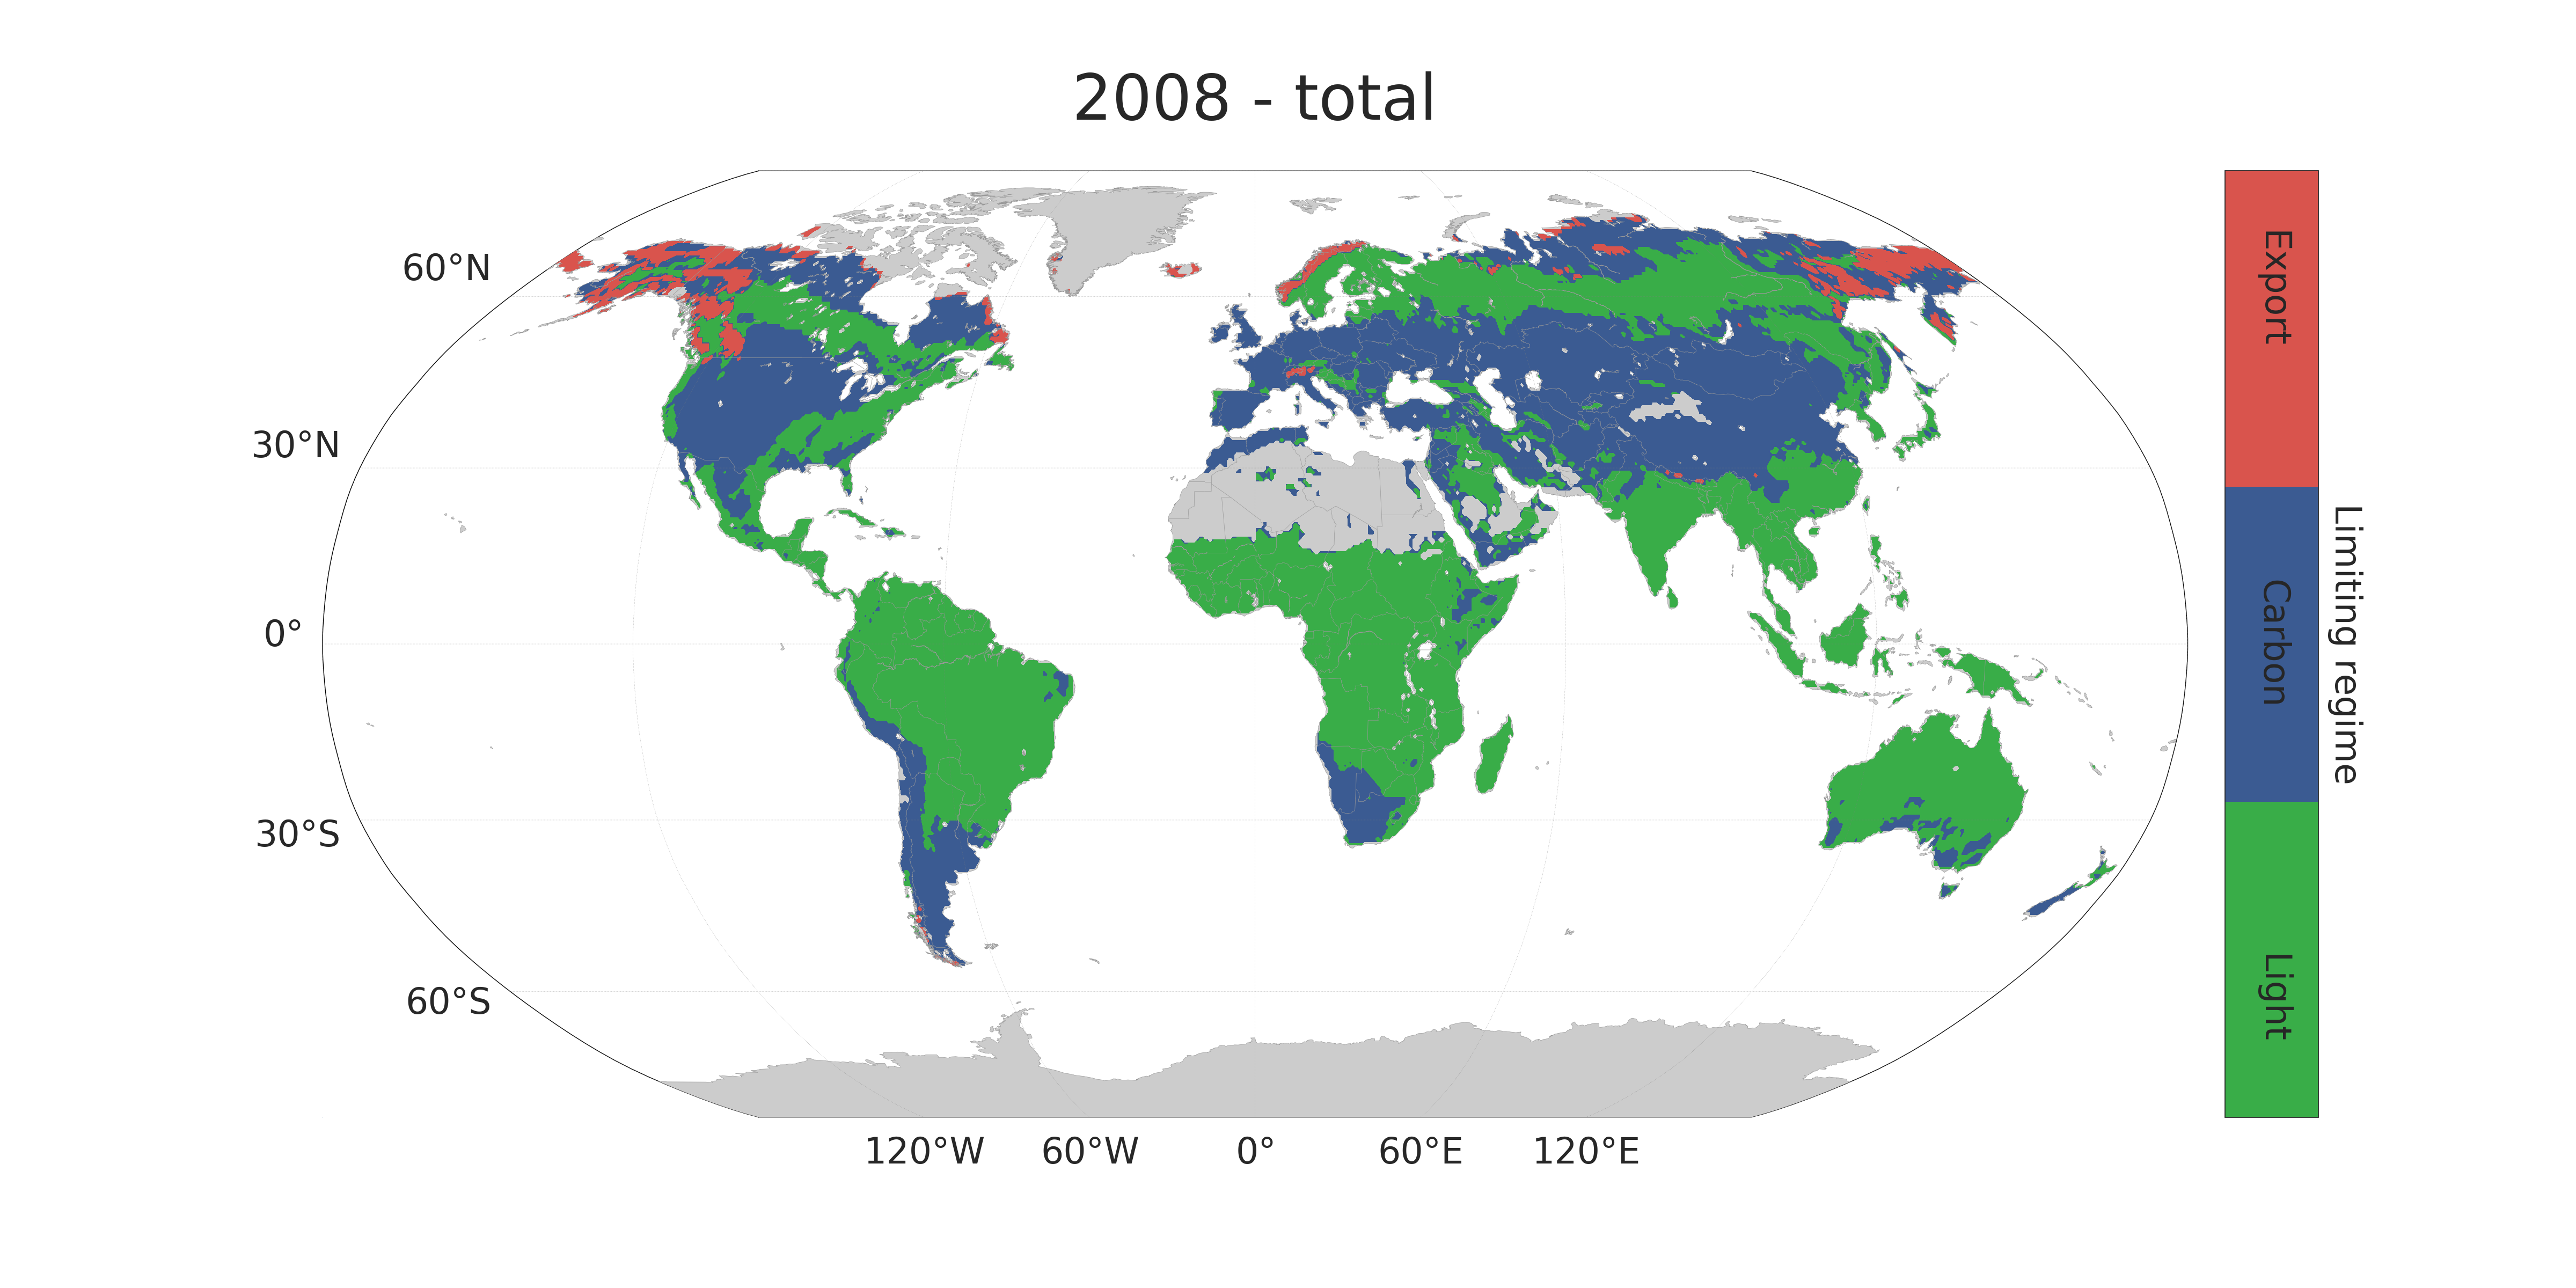
\includegraphics[width=0.5\textwidth]{/home/mn811042/Thesis/chapter6/figures_ofi/Farquhar_year_total_opt5_integral.png}}
\subfloat[Opt 5 clump]{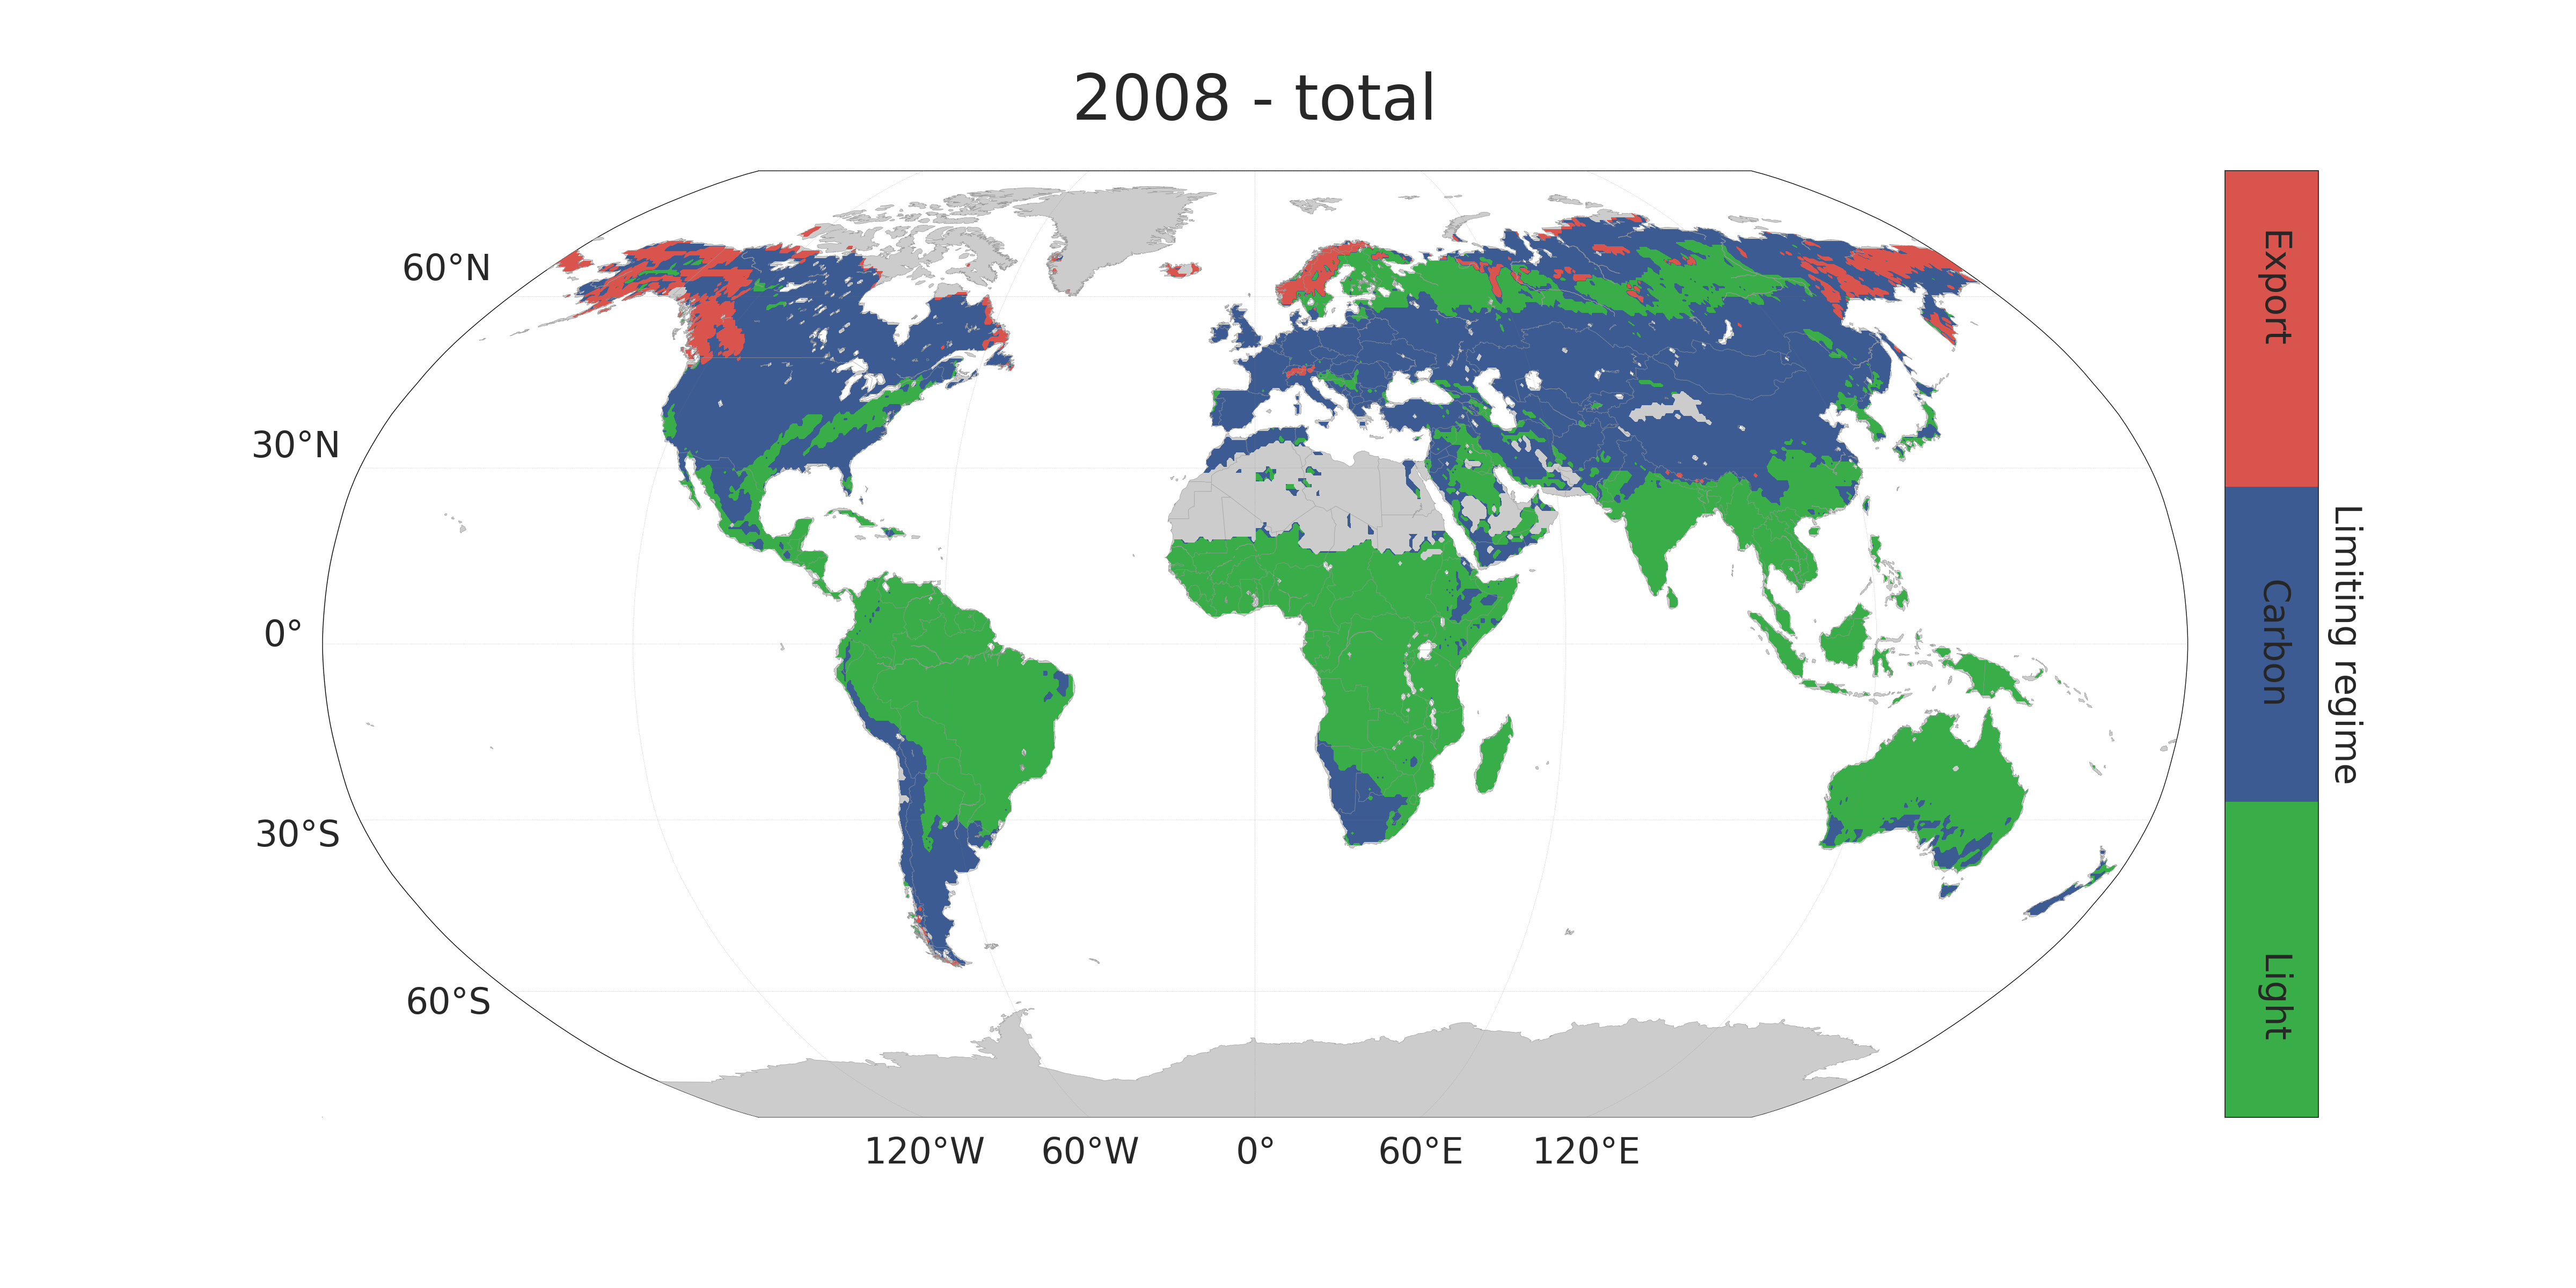
\includegraphics[width=0.5\textwidth]{/home/mn811042/Thesis/chapter6/figures_ofi/Farquhar_year_total_opt5_clump_integral.png}}
\end{tabular}
\subfloat[Difference]{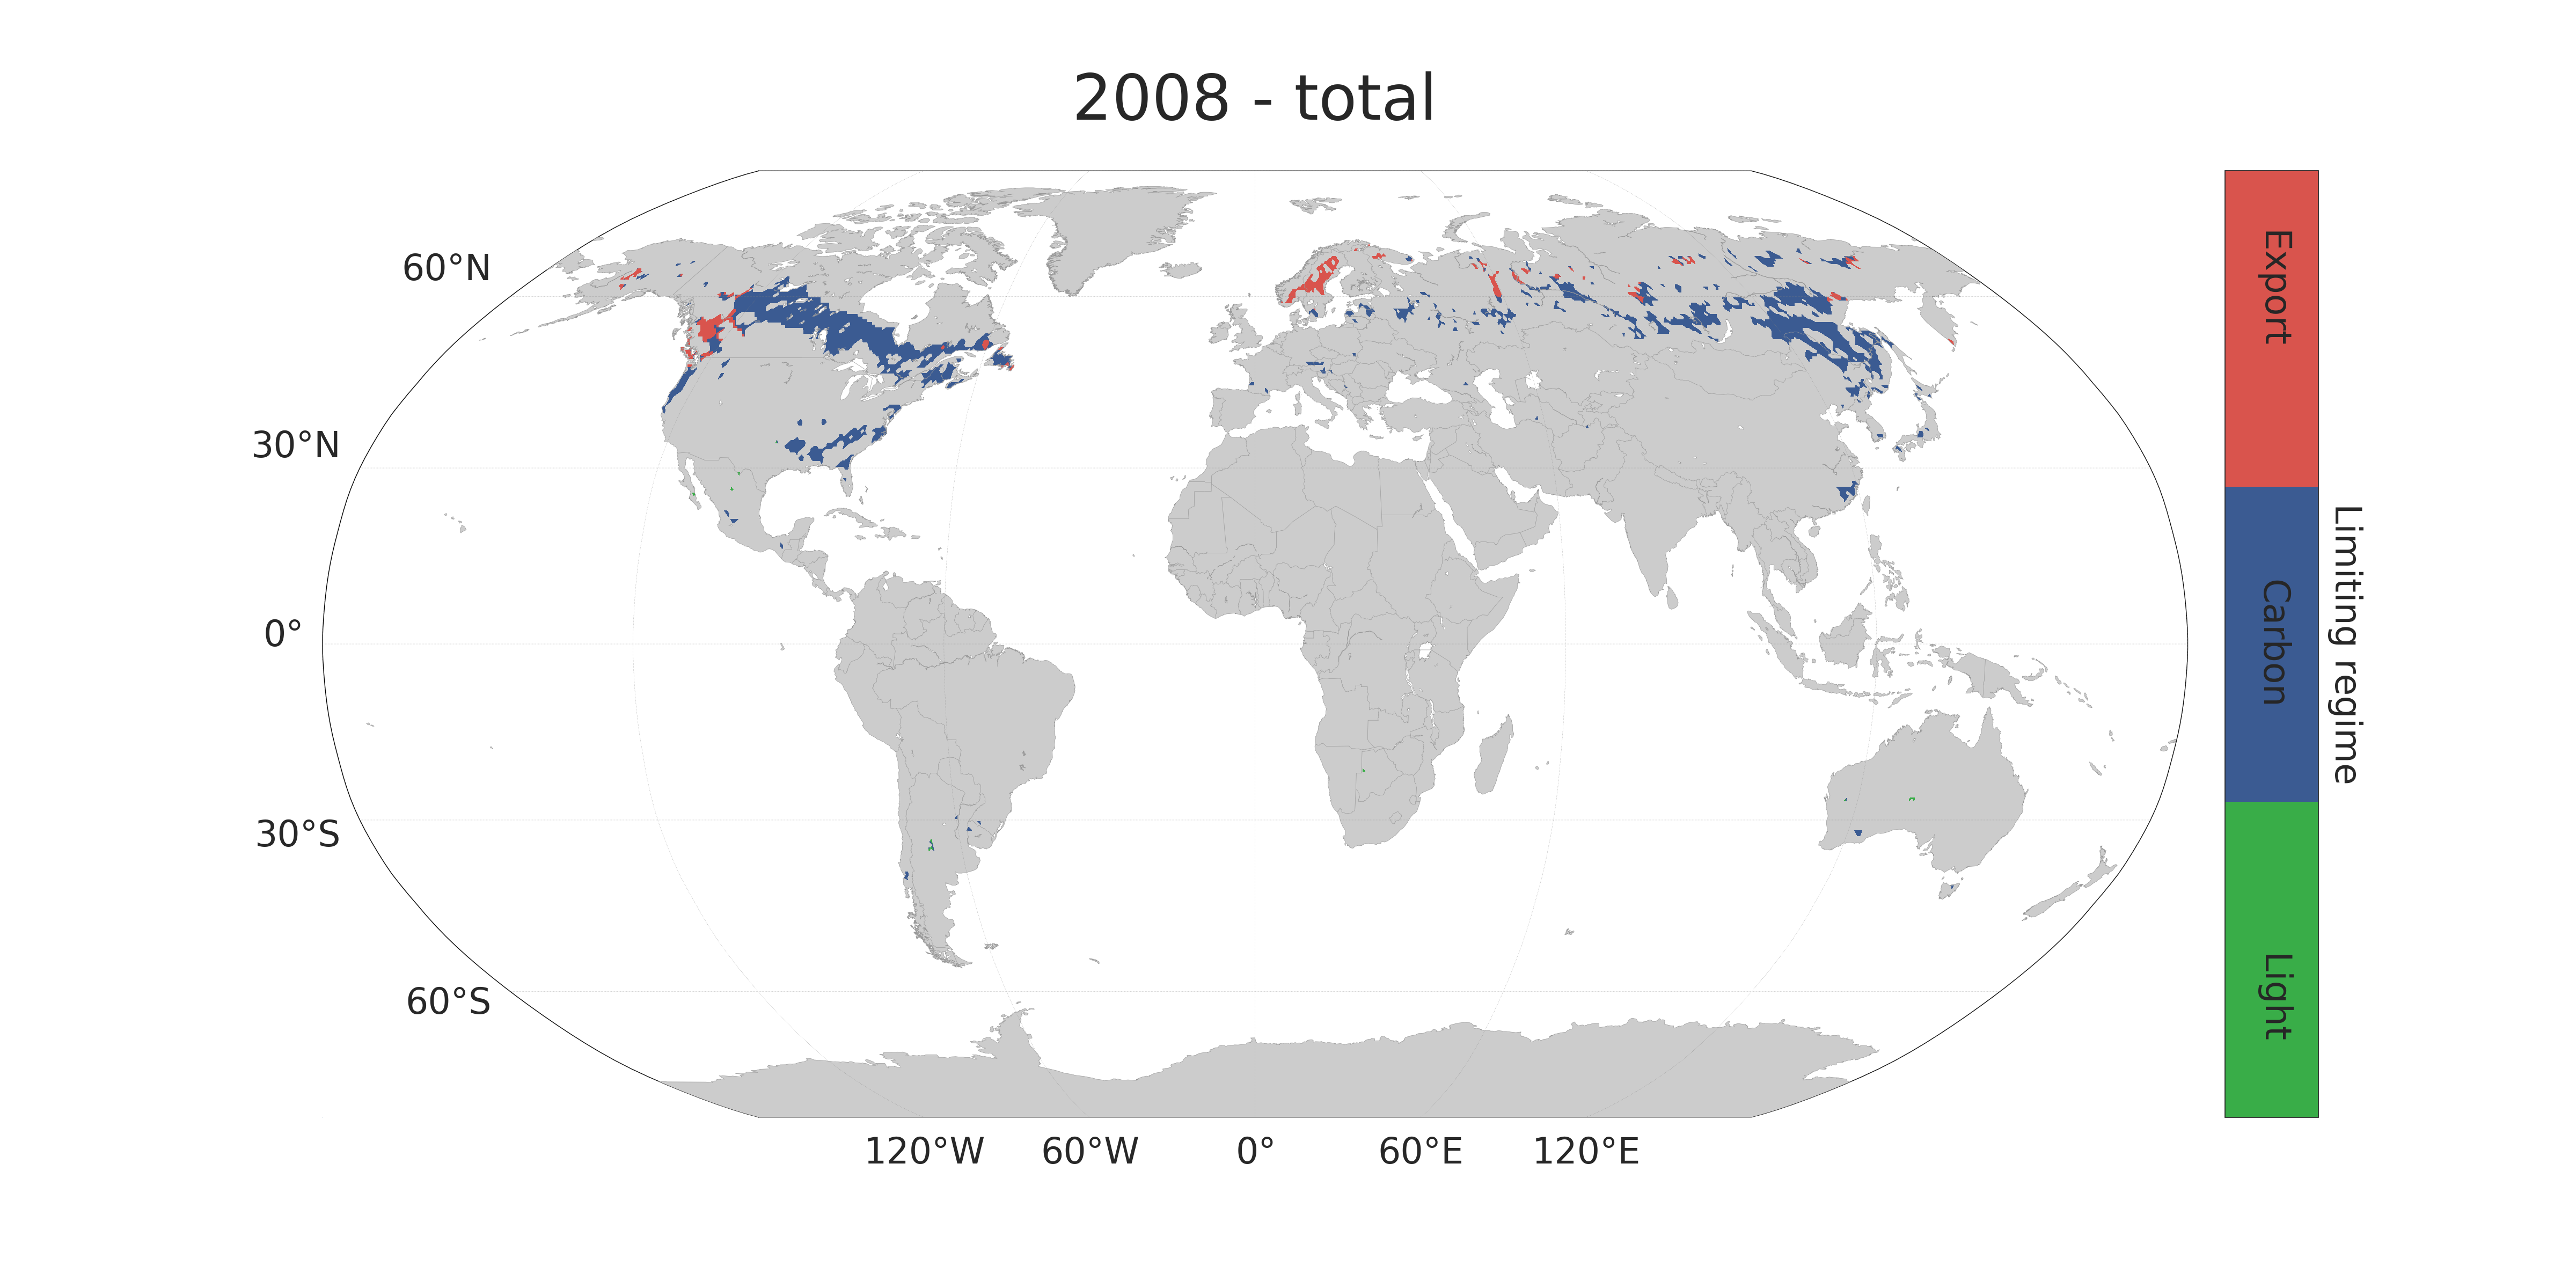
\includegraphics[width=1.0\textwidth]{/home/mn811042/Thesis/chapter6/figures_ofi/Farquhar_year_total_opt5_clump_integral_diff.png}}
\caption{Spatial distribution of the Farquhar limiting regimes of photosynthesis for the year of 2008 according to a. the default JULES, and b. JULES with clumping; c. shows the regions where the limiting regimes changed from the default version to the version with clumping in JULES. The actual limiting regimes of difference are associated with the version considering canopuy structure.}
\label{f:limiting_regimes_spatial_global}
\end{figure}

%These comments below were adapted from http://globalforestatlas.yale.edu/boreal-forest/boreal-ecoregions-ecology/boreal-forest-ecology

Boreal forests must withstand very harsh conditions, which include long winters and short summers. Also these forests are located in very high latitudes which means very high Sun zenith angles all over the year, which can be translated to very limited amounts of total radiation. Therefore tree species that inhabit boreal forests have adaptations that help them to maximise photosynthesis under such a naturally light limited enviroment. Boreal forests are mostly dominated by needle-leaved species and most of them are evergreen conifers, allowing these trees to begin photosynthesizing early in the spring when temperatures are favorable, rather than wasting valuable time to grow new leaves. These needled coniferous species also display more leaves per unit area than deciduous broadleaved species do. The needles tend to be angled to the Sun, allowing them to use light for photosynthesis more efficiently, which is beneficial where cold temperatures already constrain photosynthesis. Most conifers are cone-shaped, which allows branches and needles to receive more direct sunlight without shading other branches. Having a conical shape is especially useful for receiving sunlight that comes from a steep angle at these high boreal latitudes.

In fact, it is well documented that needle-leaf trees evolved under inhospitable climate conditions with low availability of radiation, and therefore they way they assimilate carbon should not be limited by light availabilty, but other conditions, e.g., extreme cold temperatures, or very dry summers. Of course the adaptations of the boreal forests are not only constrained to lower light availability. For example, the narrowness of the needles reduces the surface area of water loss, which is important where cold and dry conditions prevent trees from replenishing their water from the ground. Needle-leaves also have a thick waxy coating called a cuticle that helps prevent water loss and protects inner leaf architecture from desiccation and abrasive winds. Other adaptations are reflected in their wood anatomy and water transport system, which is well suited to withstand cold and dry conditions. In fact, broadleaf species tend to outcompete conifers on more favorable sites, thus relegating conifers to the more inhospitable sites. Also its shape prevents snow from piling on branches and it helps to keep these shallow-rooted trees sturdy in windy conditions.

Althought it is hard to say what is the average photosynthesis limiting regime according to the Farquhar model for Boreal forests, it is unlikely that these ecosystems would be light limited given their evolutionary characteristics of canopy and leaf architecture. Perhaps most importantly, it is not straighforward the relation between climatic variables and the Farquhar limiting regimes of photosynthesis. 

In order to estimate the consistency between the limiting regimes according to the Farquhar model and the climatic variables constratining photosynthesis, the MTE-GPP product together with the WFDEI reanalysis dataset of shortwave incident radiation, air temperature, and the CRU precipitation products were monthly correlated at 0.5$^{\circ}$ gridbox level for the year of 2008 over the globe. The variability caused by each climatic factor (i.e., radiation, temperature, and precipitation) is assessed through the square of monthly temporal correlation coefficients between the MTE-GPP product and the climatic controls. Figure~\ref{f:climatic_control_spatial_global} indicates the areas of maximum $r^2$ related to climatic drivers. 

\begin{figure}[ht!]
\centering
\begin{tabular}{lll}
\subfloat[Radiation]{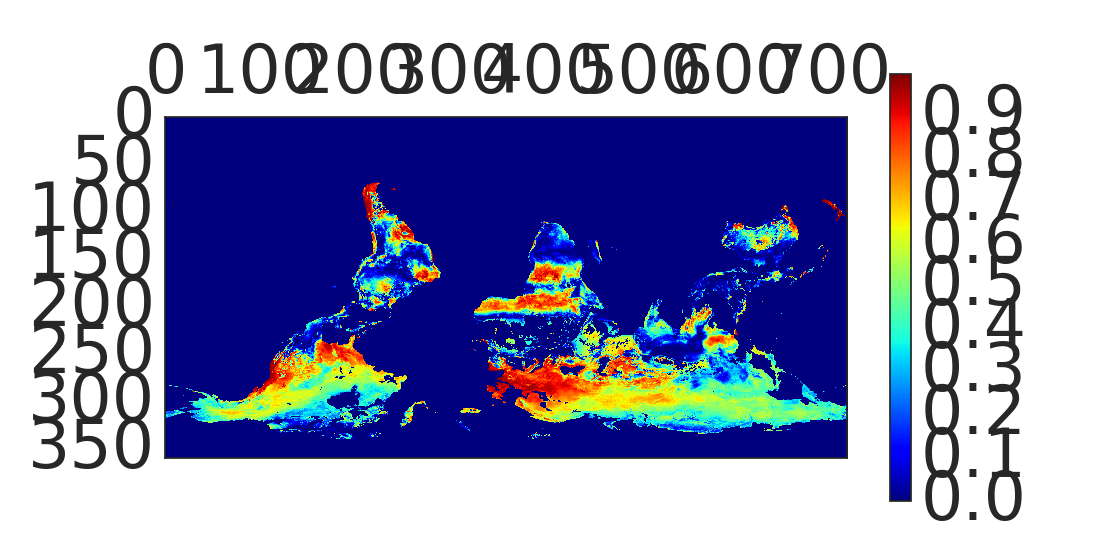
\includegraphics[width=0.33\textwidth]{/home/mn811042/Thesis/chapter6/figures_ofi/r2_gpp_mte_radiation.png}}
\subfloat[Temperature]{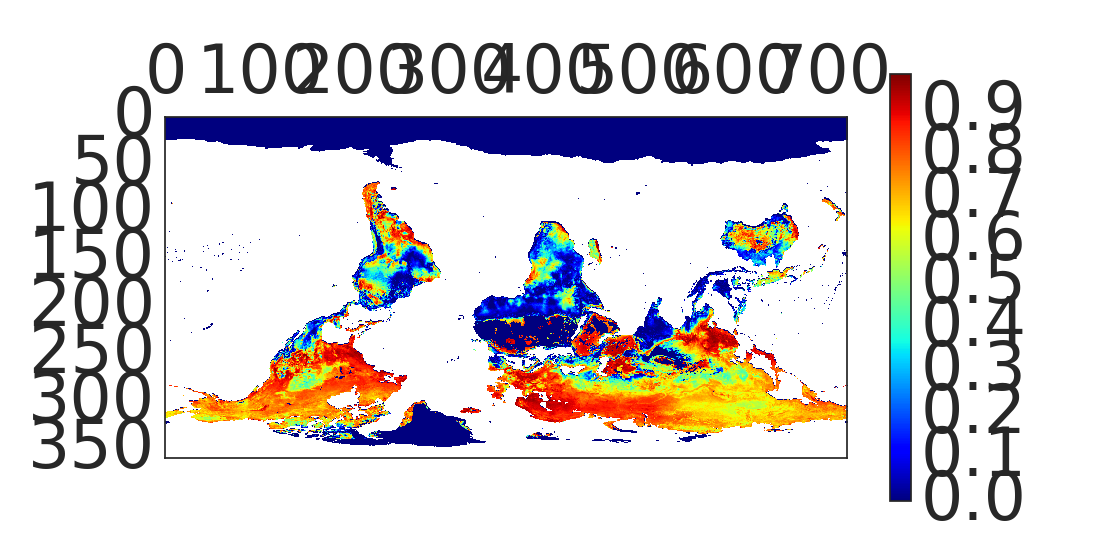
\includegraphics[width=0.33\textwidth]{/home/mn811042/Thesis/chapter6/figures_ofi/r2_gpp_mte_temp.png}}
\subfloat[Precipitation]{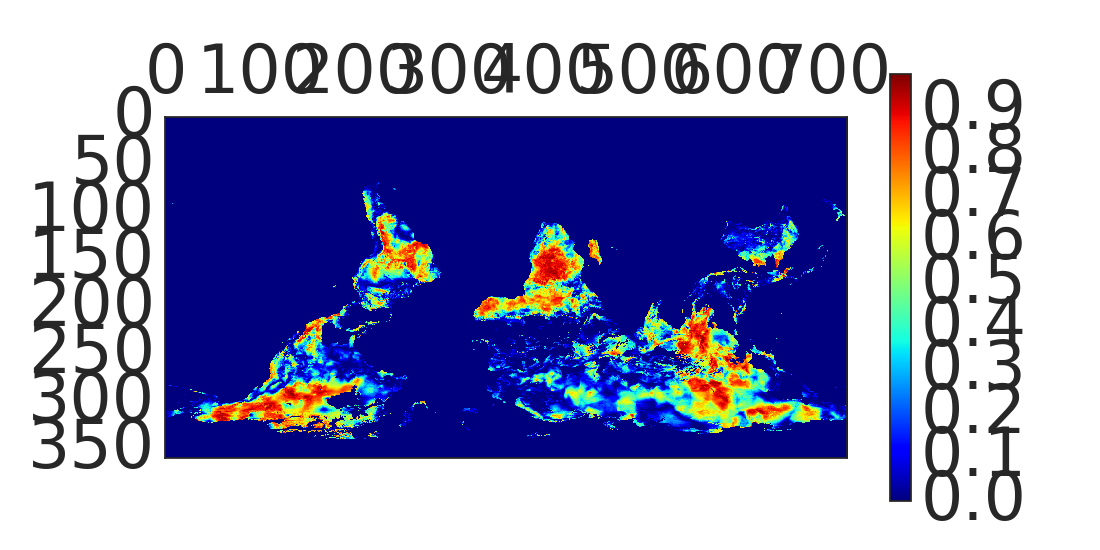
\includegraphics[width=0.33\textwidth]{/home/mn811042/Thesis/chapter6/figures_ofi/r2_gpp_mte_precip.png}}
\end{tabular}
{\includegraphics[width=1.0\textwidth]{/home/mn811042/Thesis/chapter6/figures_ofi/Climatic_year_total_mte.png}}
\caption{Spatial distribution of climatic controls on interannual variation of GPP for the year of 2008.}
\label{f:climatic_control_spatial_global}
\end{figure}

The interannual variability of MTE-GPP over Boreal forests is mostly controlled by temperature and precipitation, and not radiation. Even though climatic factors cannot be directly translated to Farquhar limiting regimes, that is an indicator that Northern latitudes occupied by Boreal forests present photosynthesis limited by other factor than light.








\section{The impacts of clumping map on GPP}\label{section:gpp_distribution}



\begin{figure}[ht!]
\centering
\subfloat[MTE]{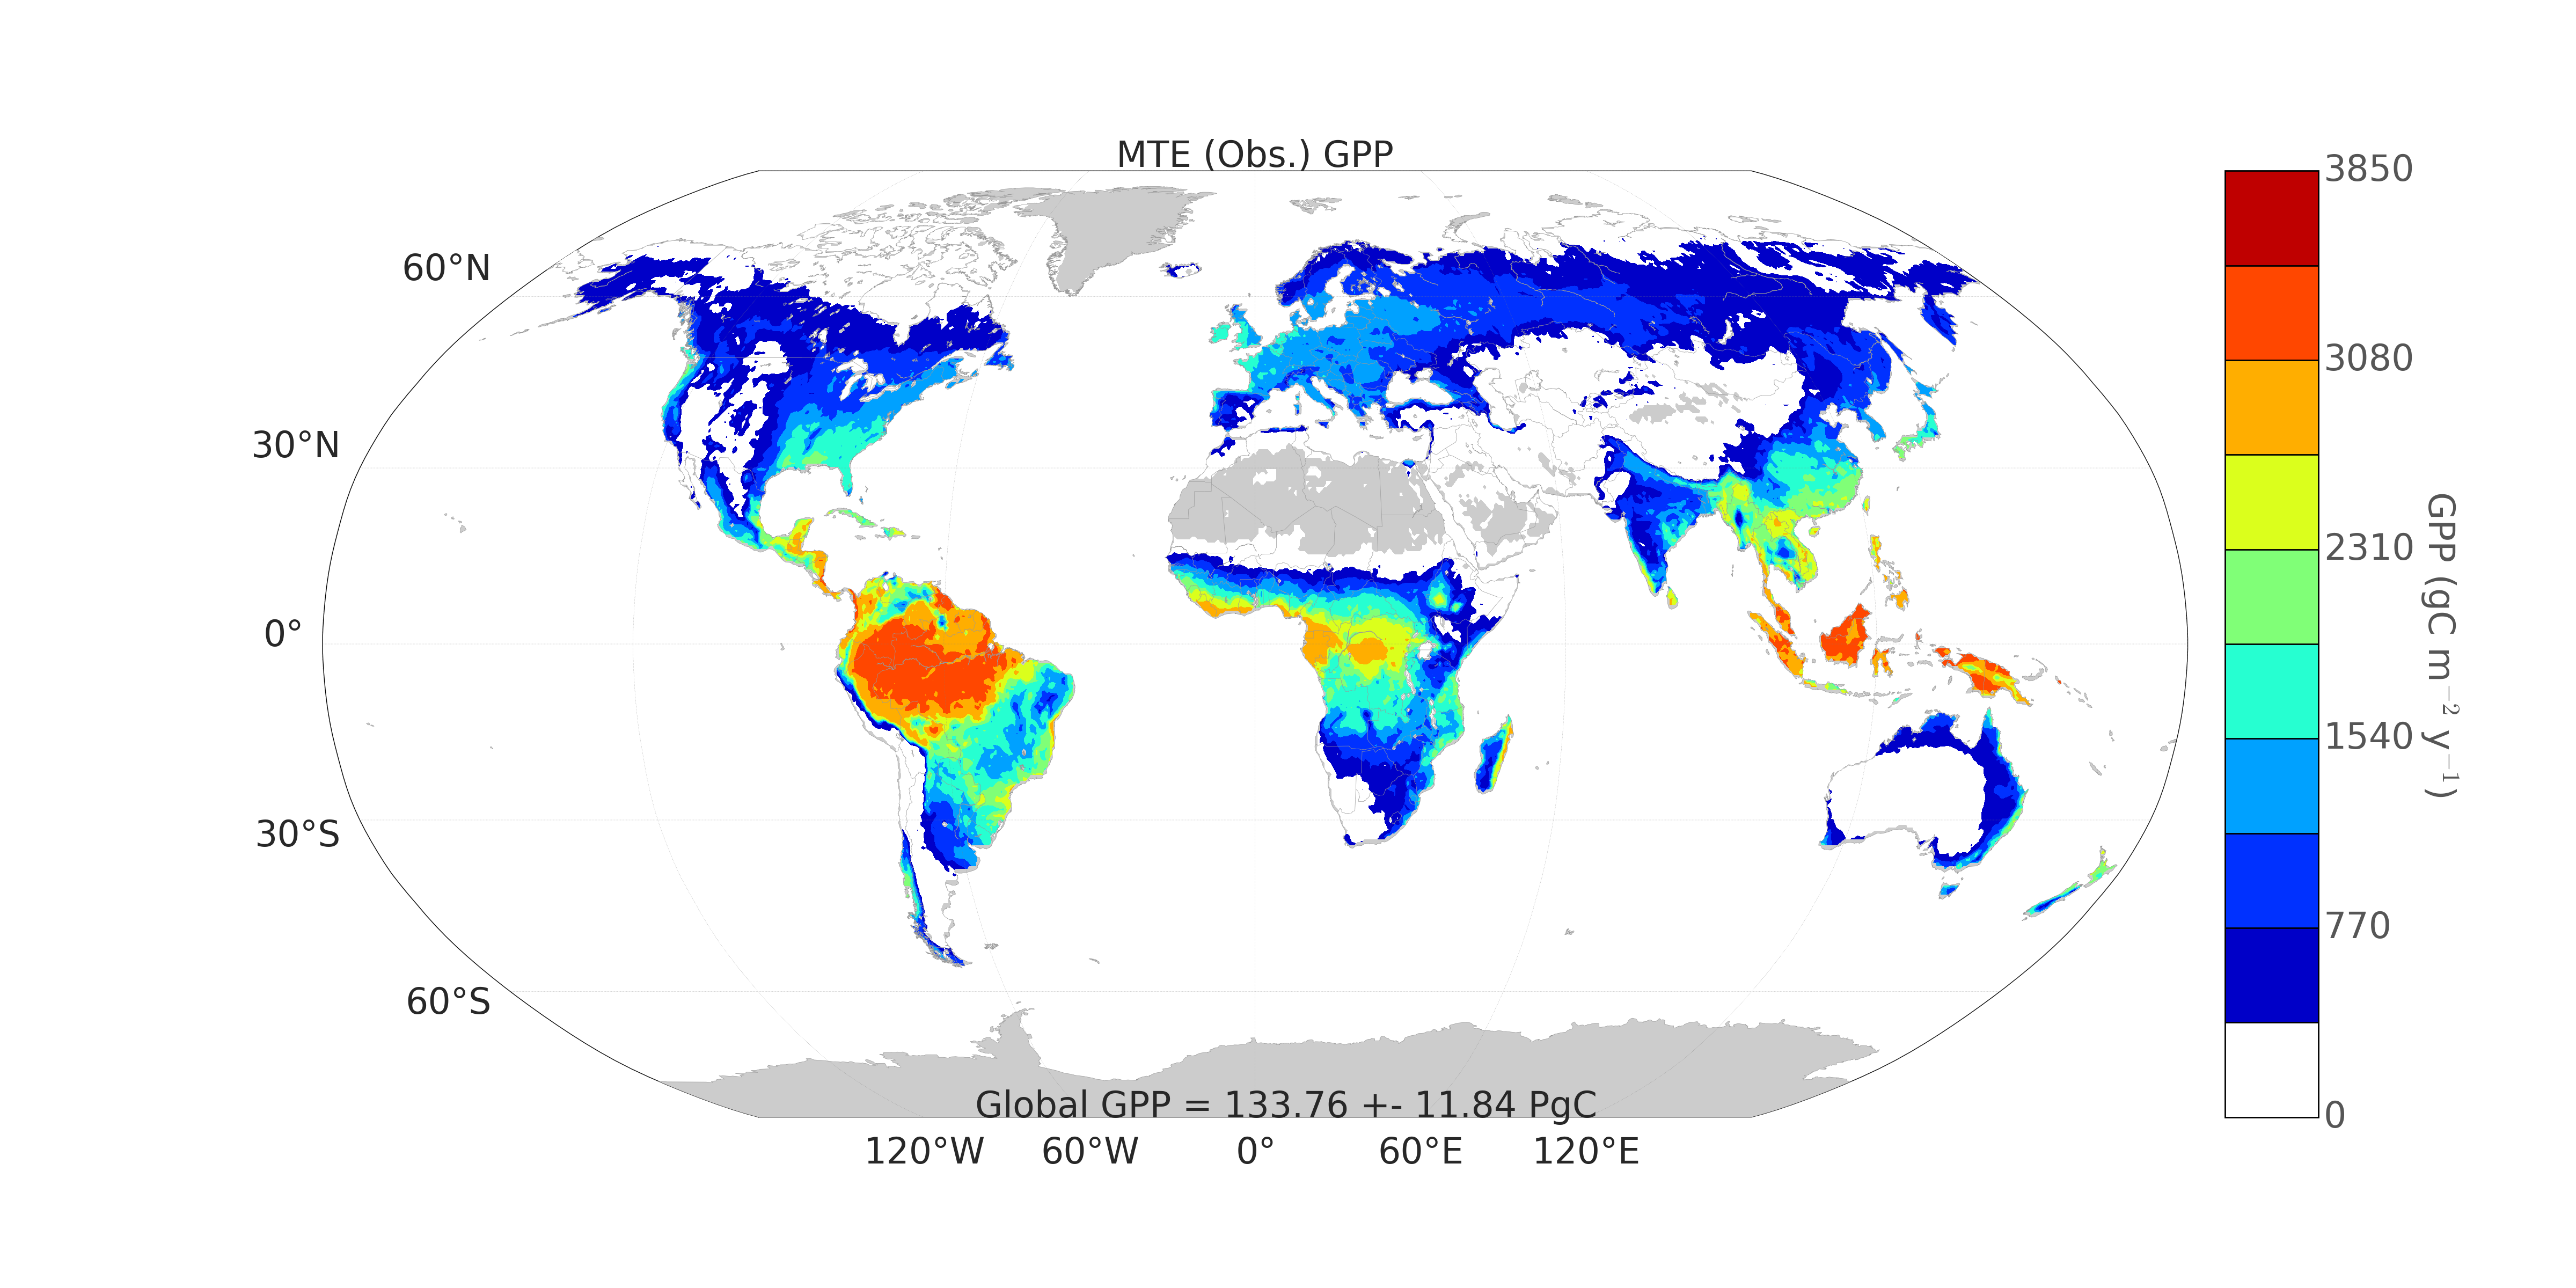
\includegraphics[width=0.8\textwidth]{/home/mn811042/Thesis/chapter6/figures_ofi/mte_0_MR_year.png}}
\begin{tabular}{ll}
\subfloat[Opt 4]{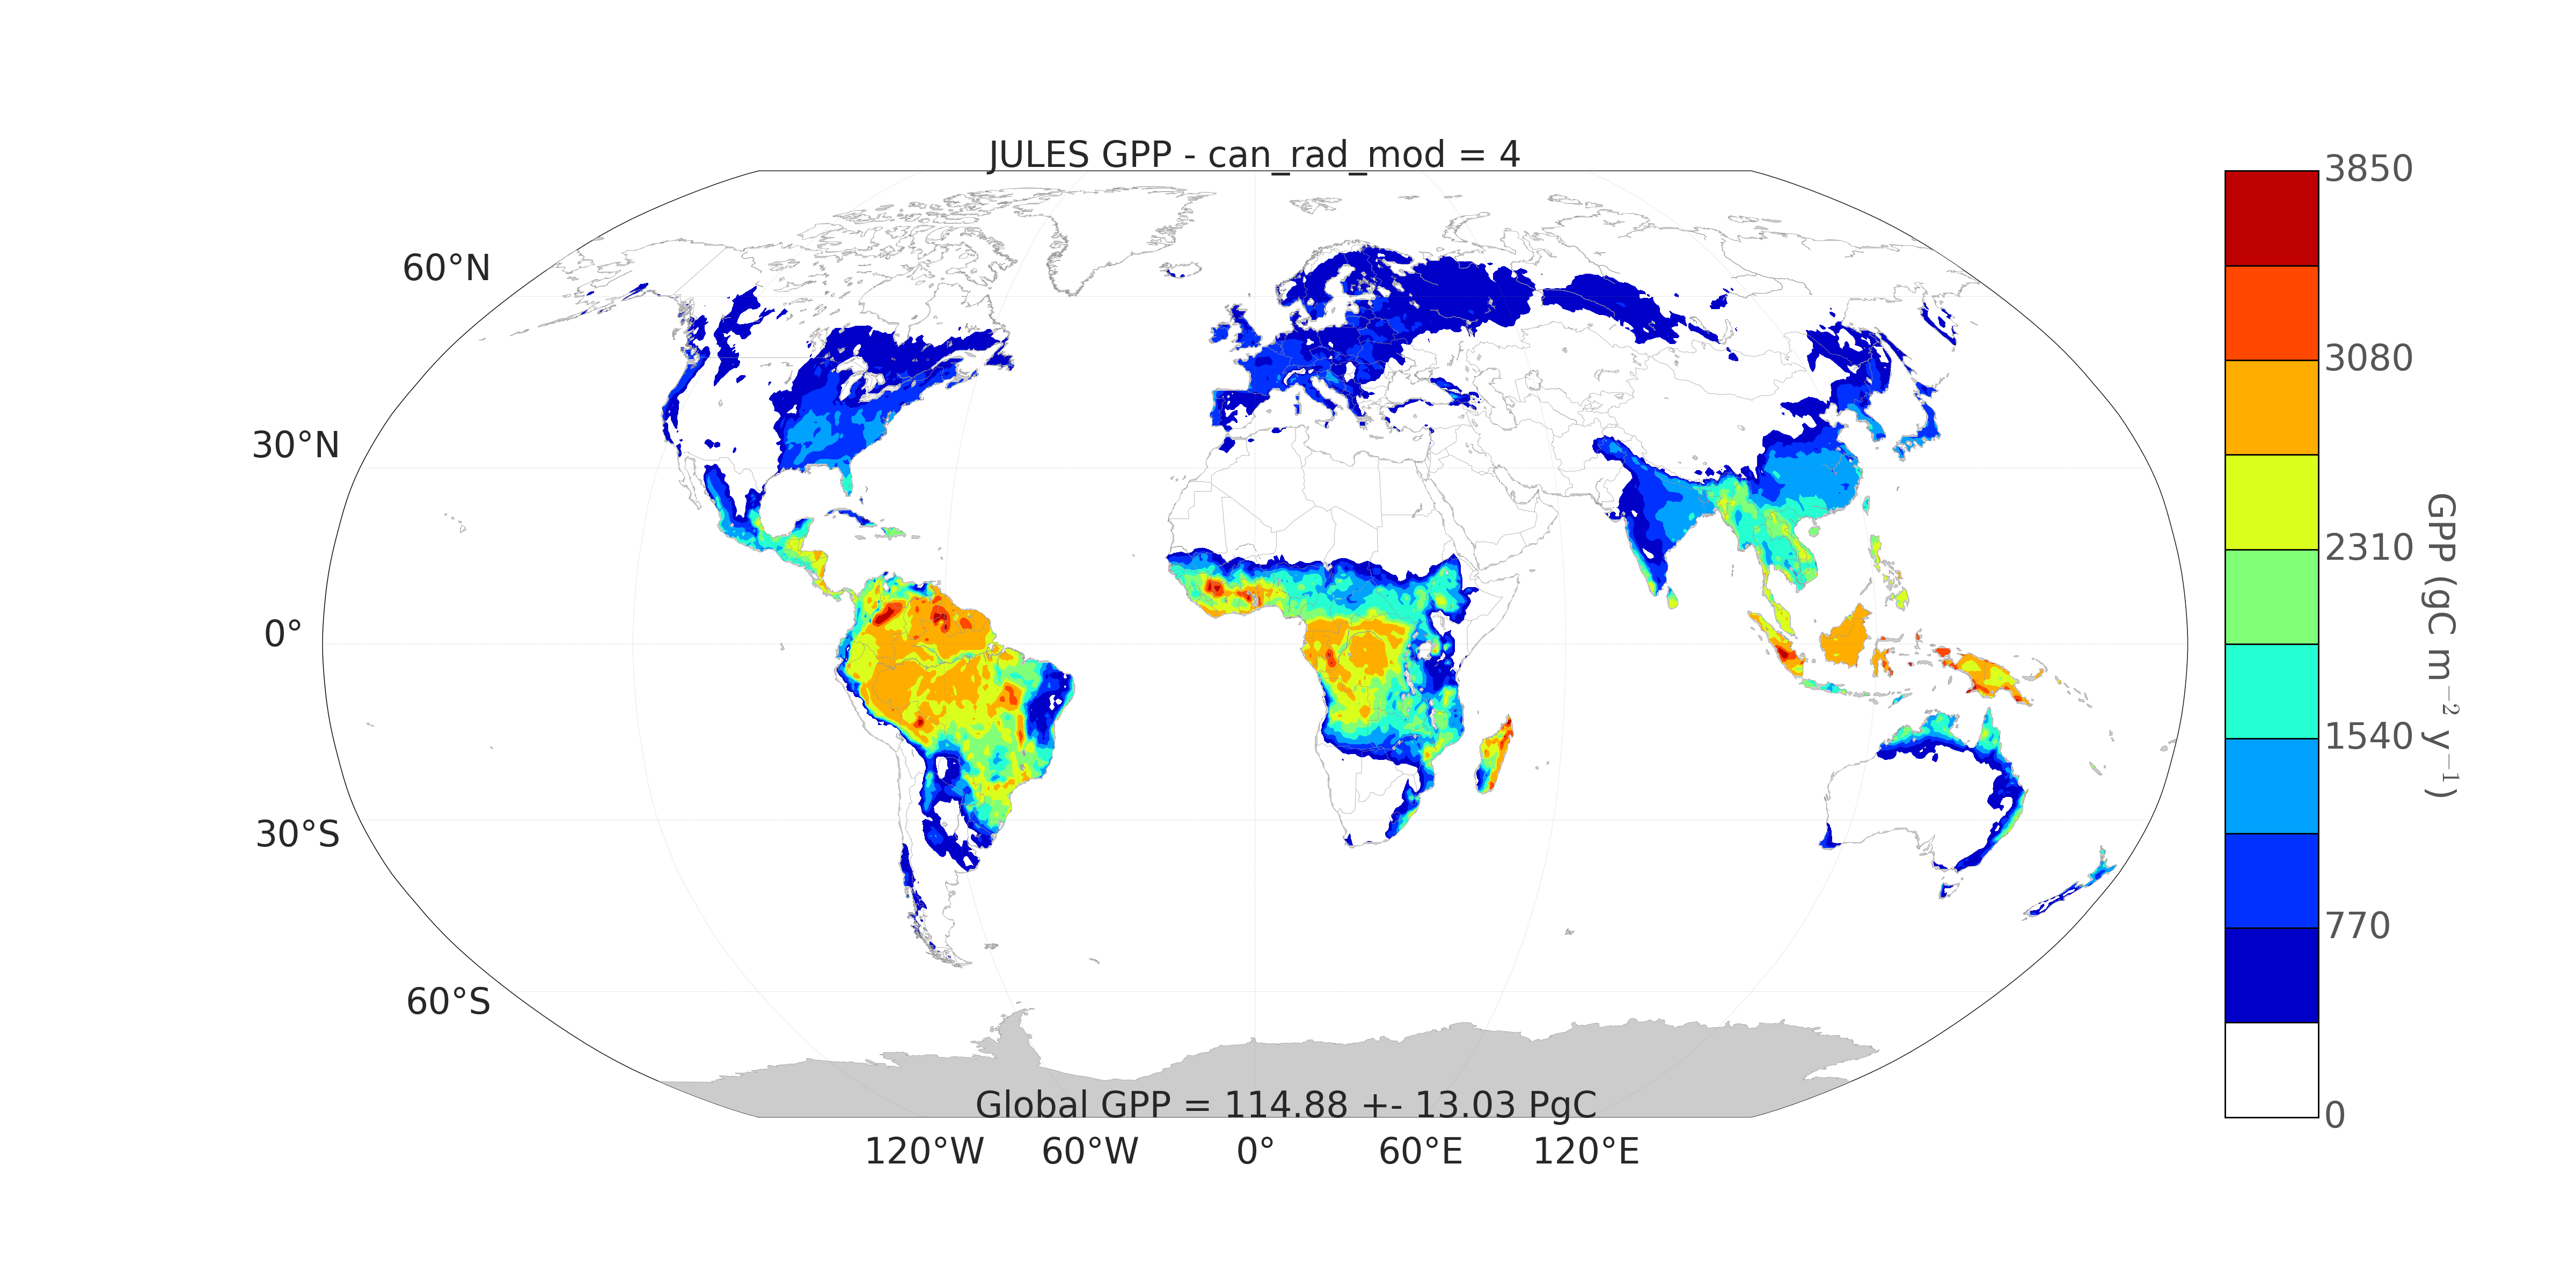
\includegraphics[width=0.5\textwidth]{/home/mn811042/Thesis/chapter6/figures_ofi/jules_opt4_year.png}}
\subfloat[Opt 4 clump]{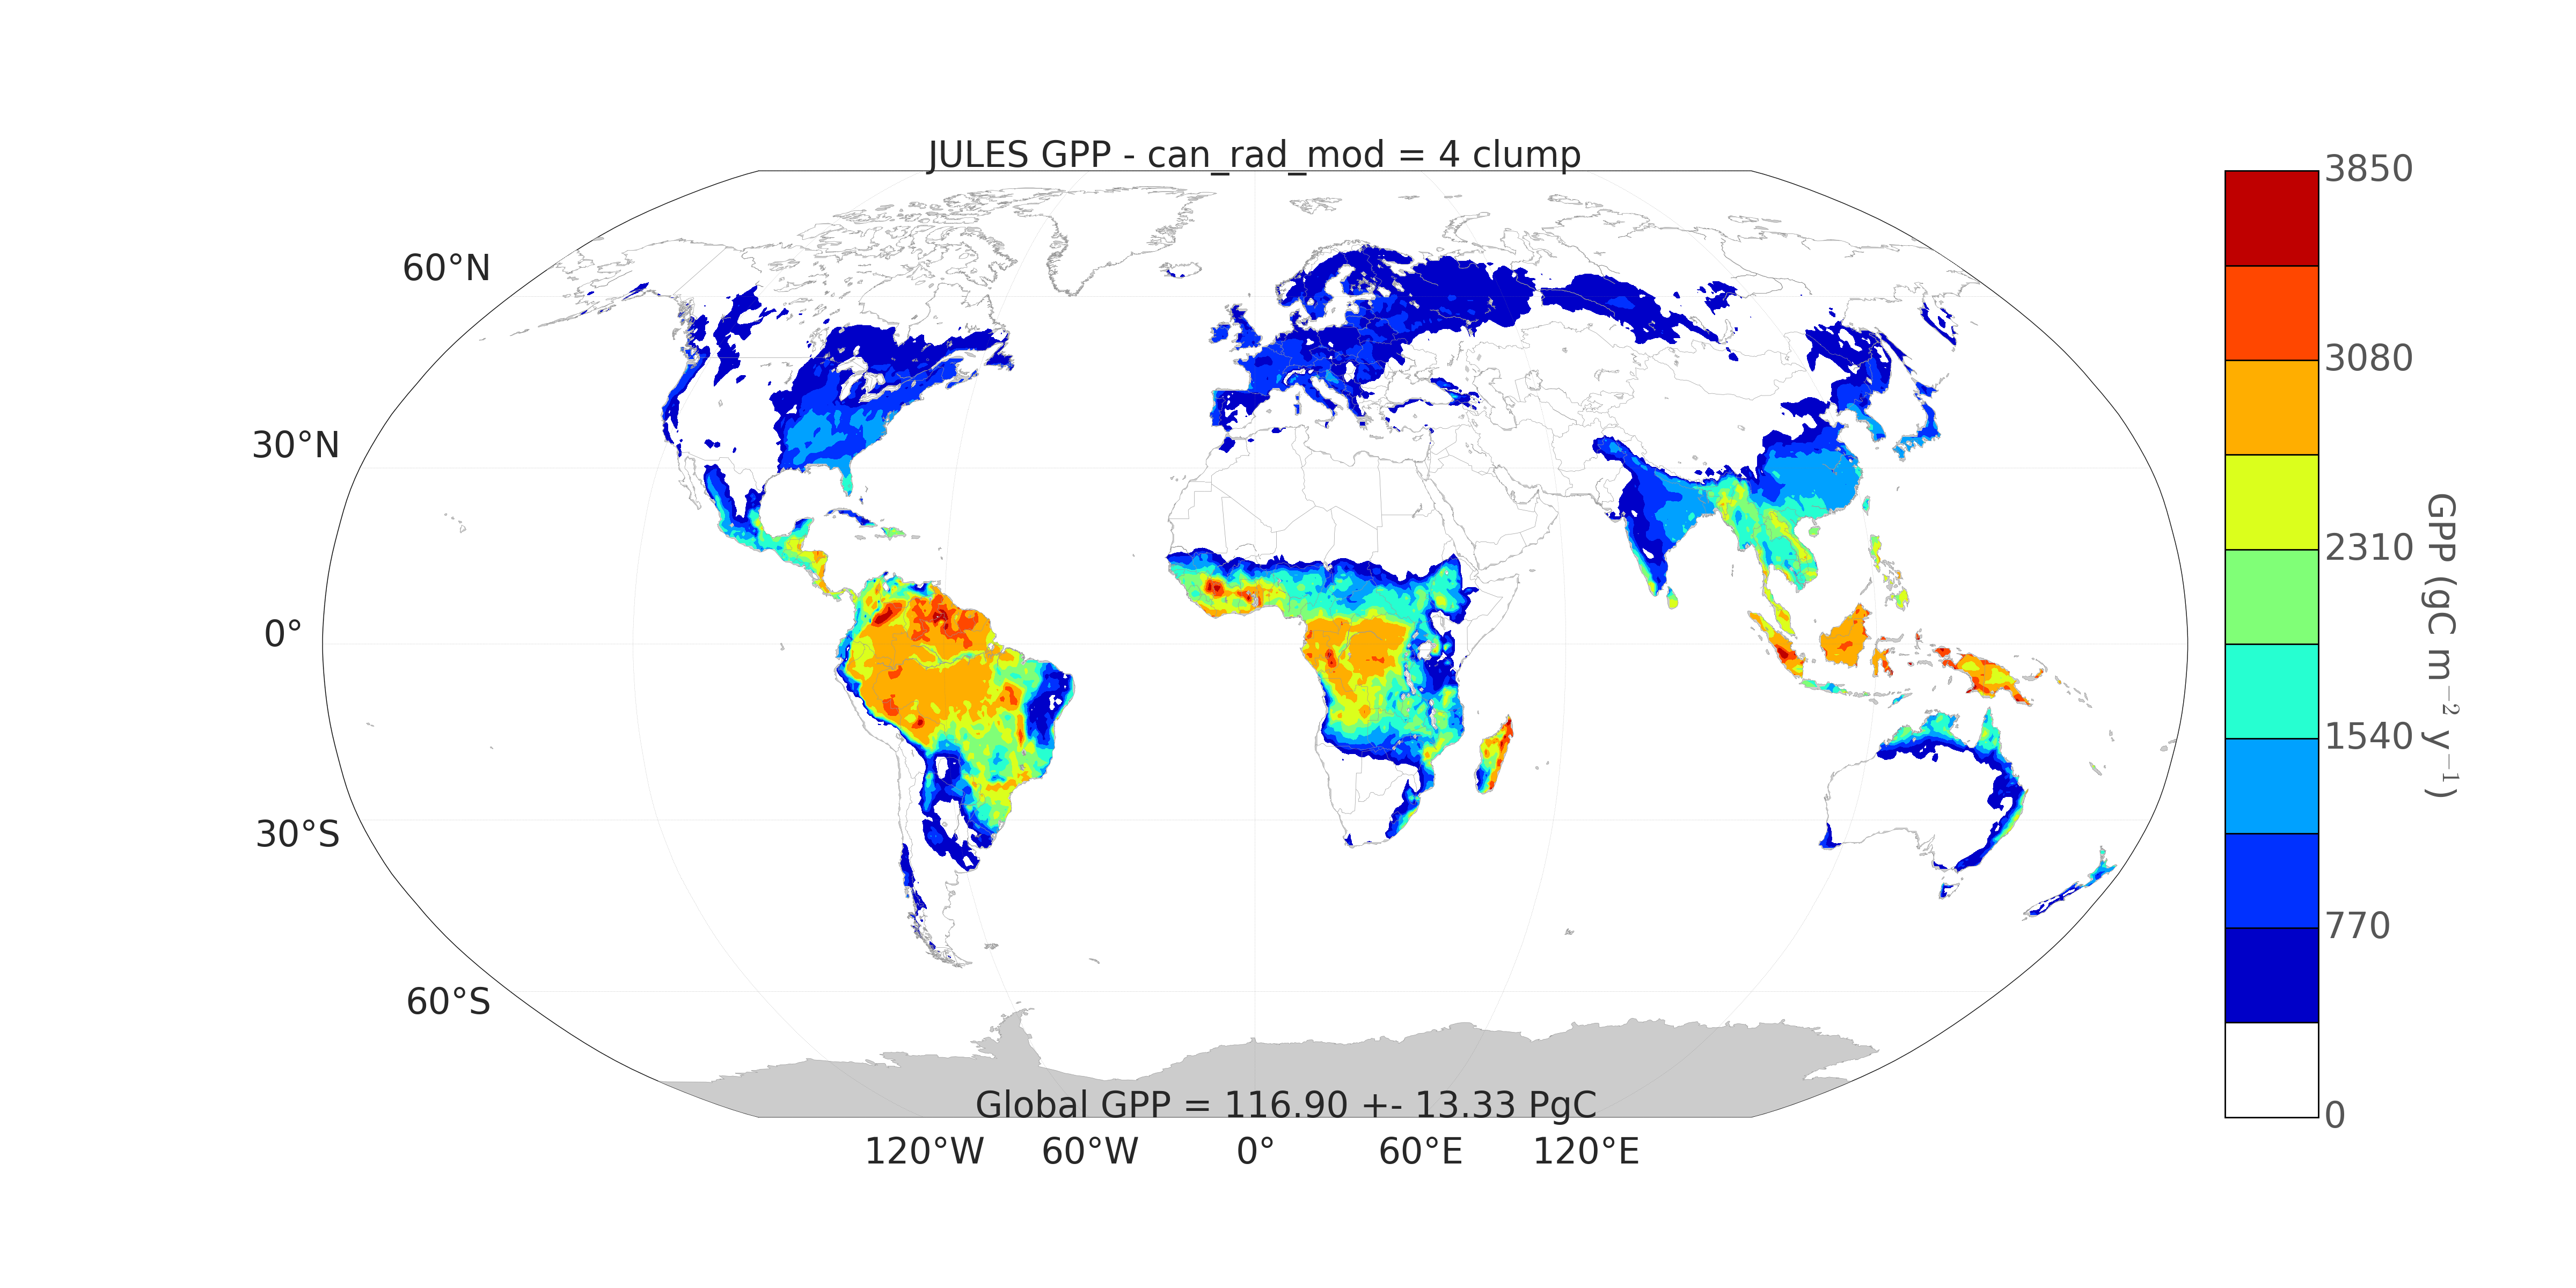
\includegraphics[width=0.5\textwidth]{/home/mn811042/Thesis/chapter6/figures_ofi/jules_opt4_clump_year.png}}
\end{tabular}
\begin{tabular}{ll}
\subfloat[Opt 5]{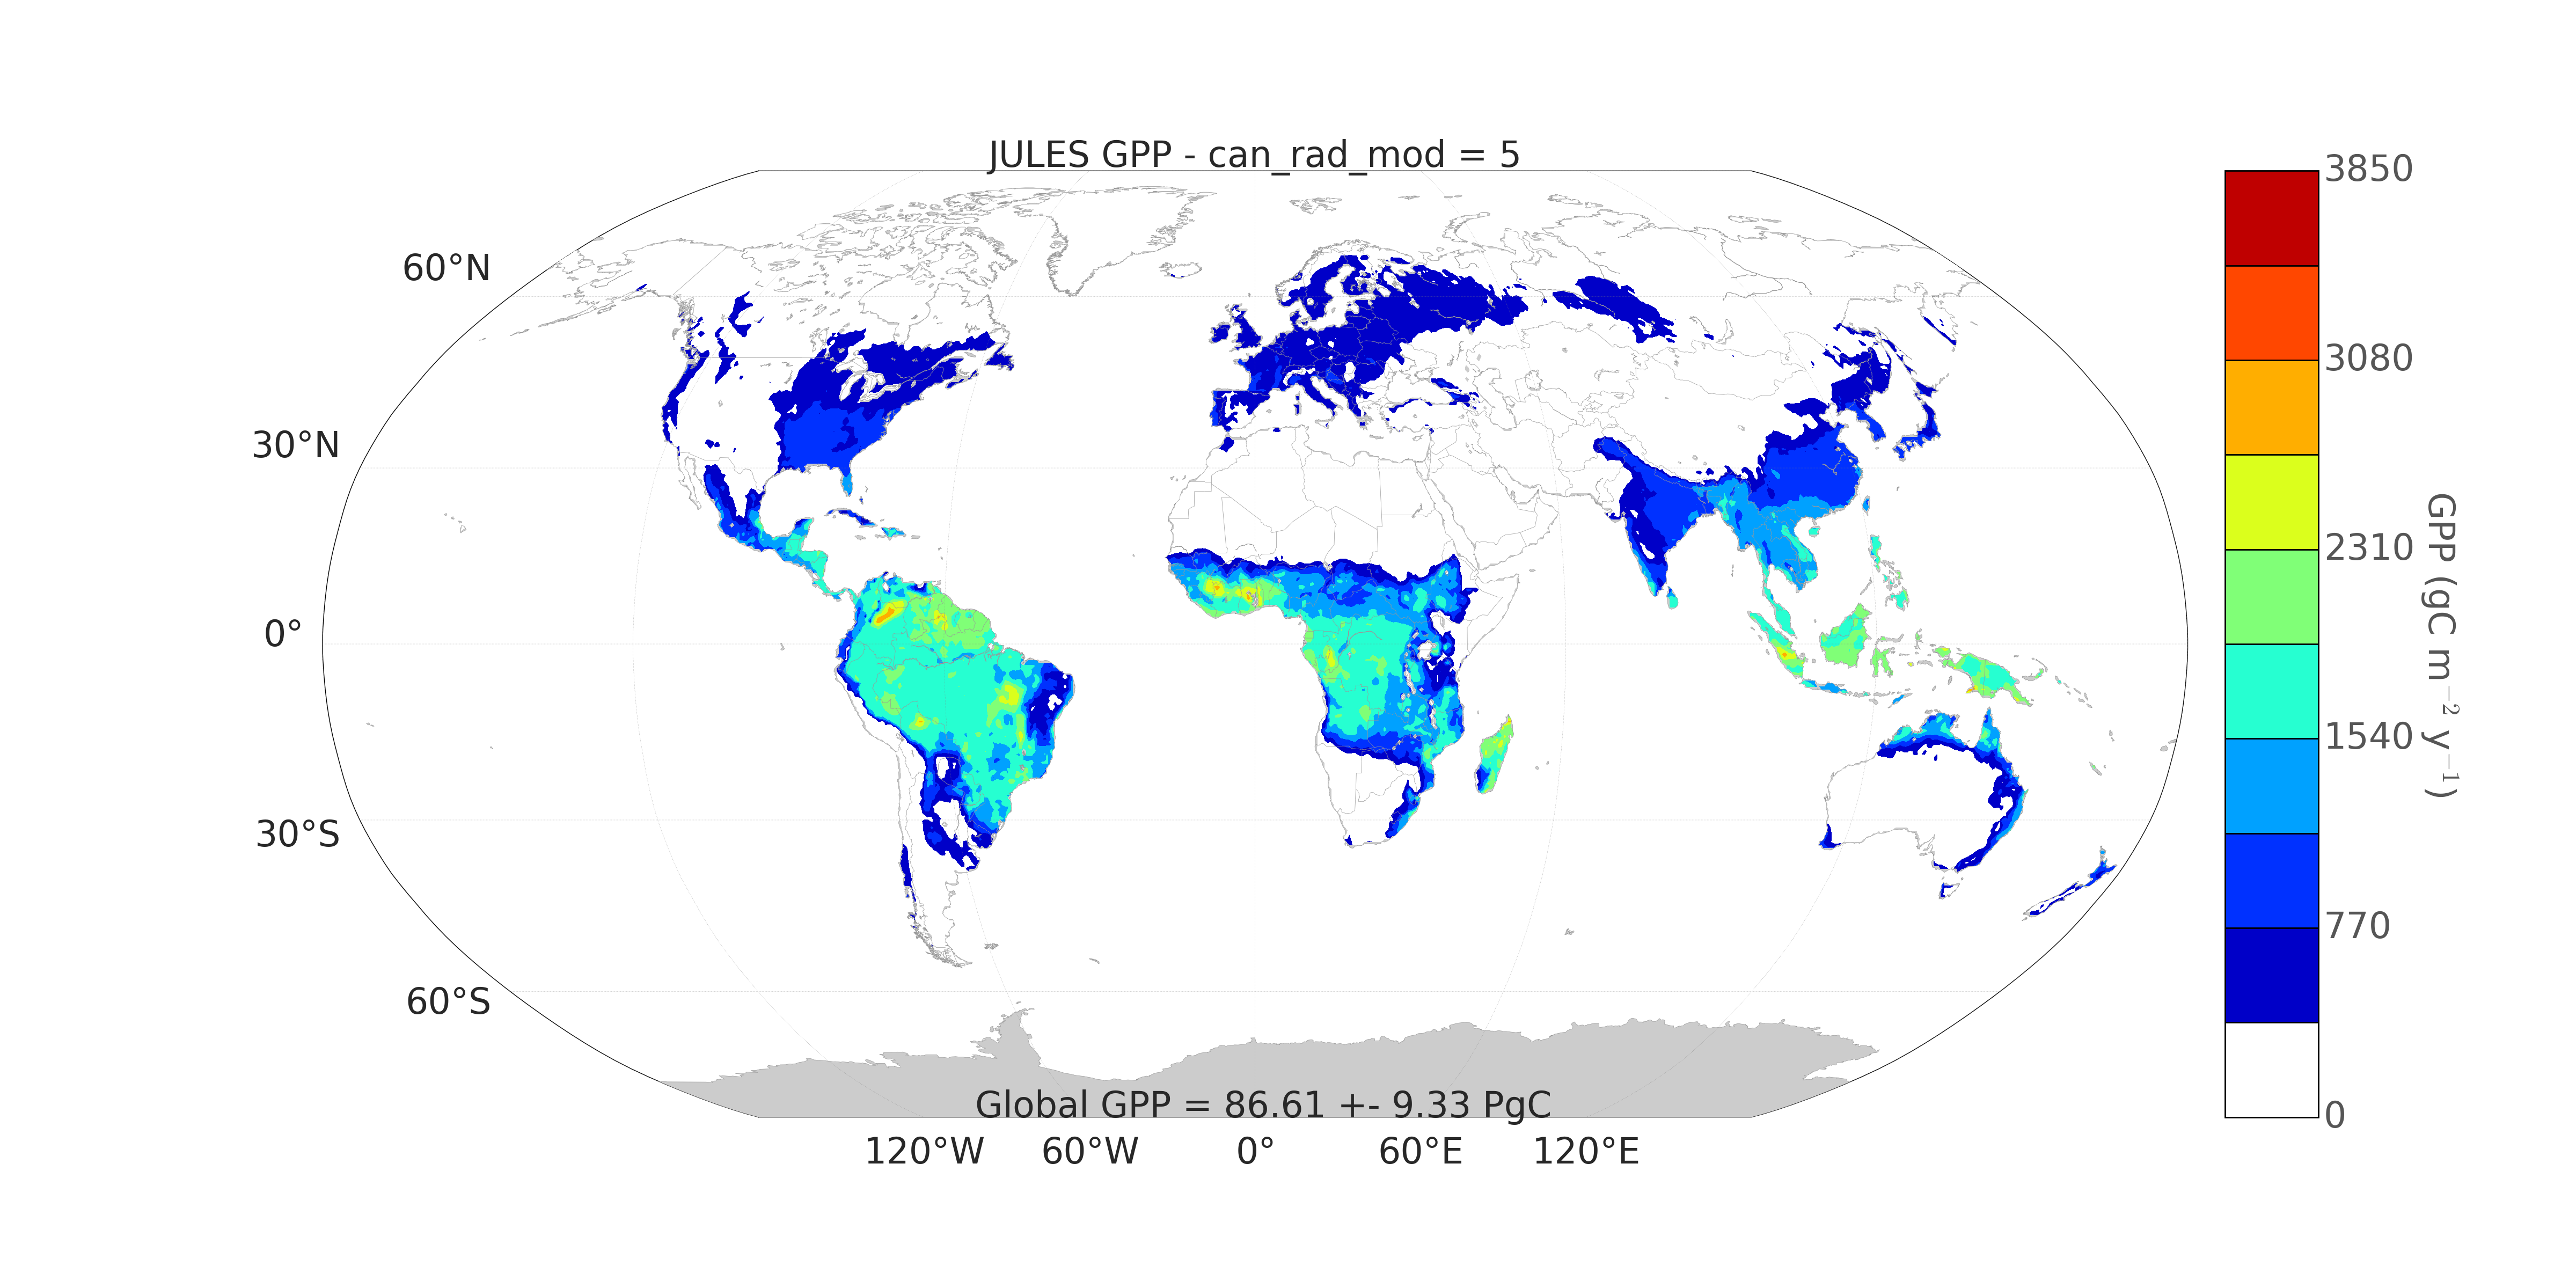
\includegraphics[width=0.5\textwidth]{/home/mn811042/Thesis/chapter6/figures_ofi/jules_opt5_year.png}}
\subfloat[Opt 5 clump]{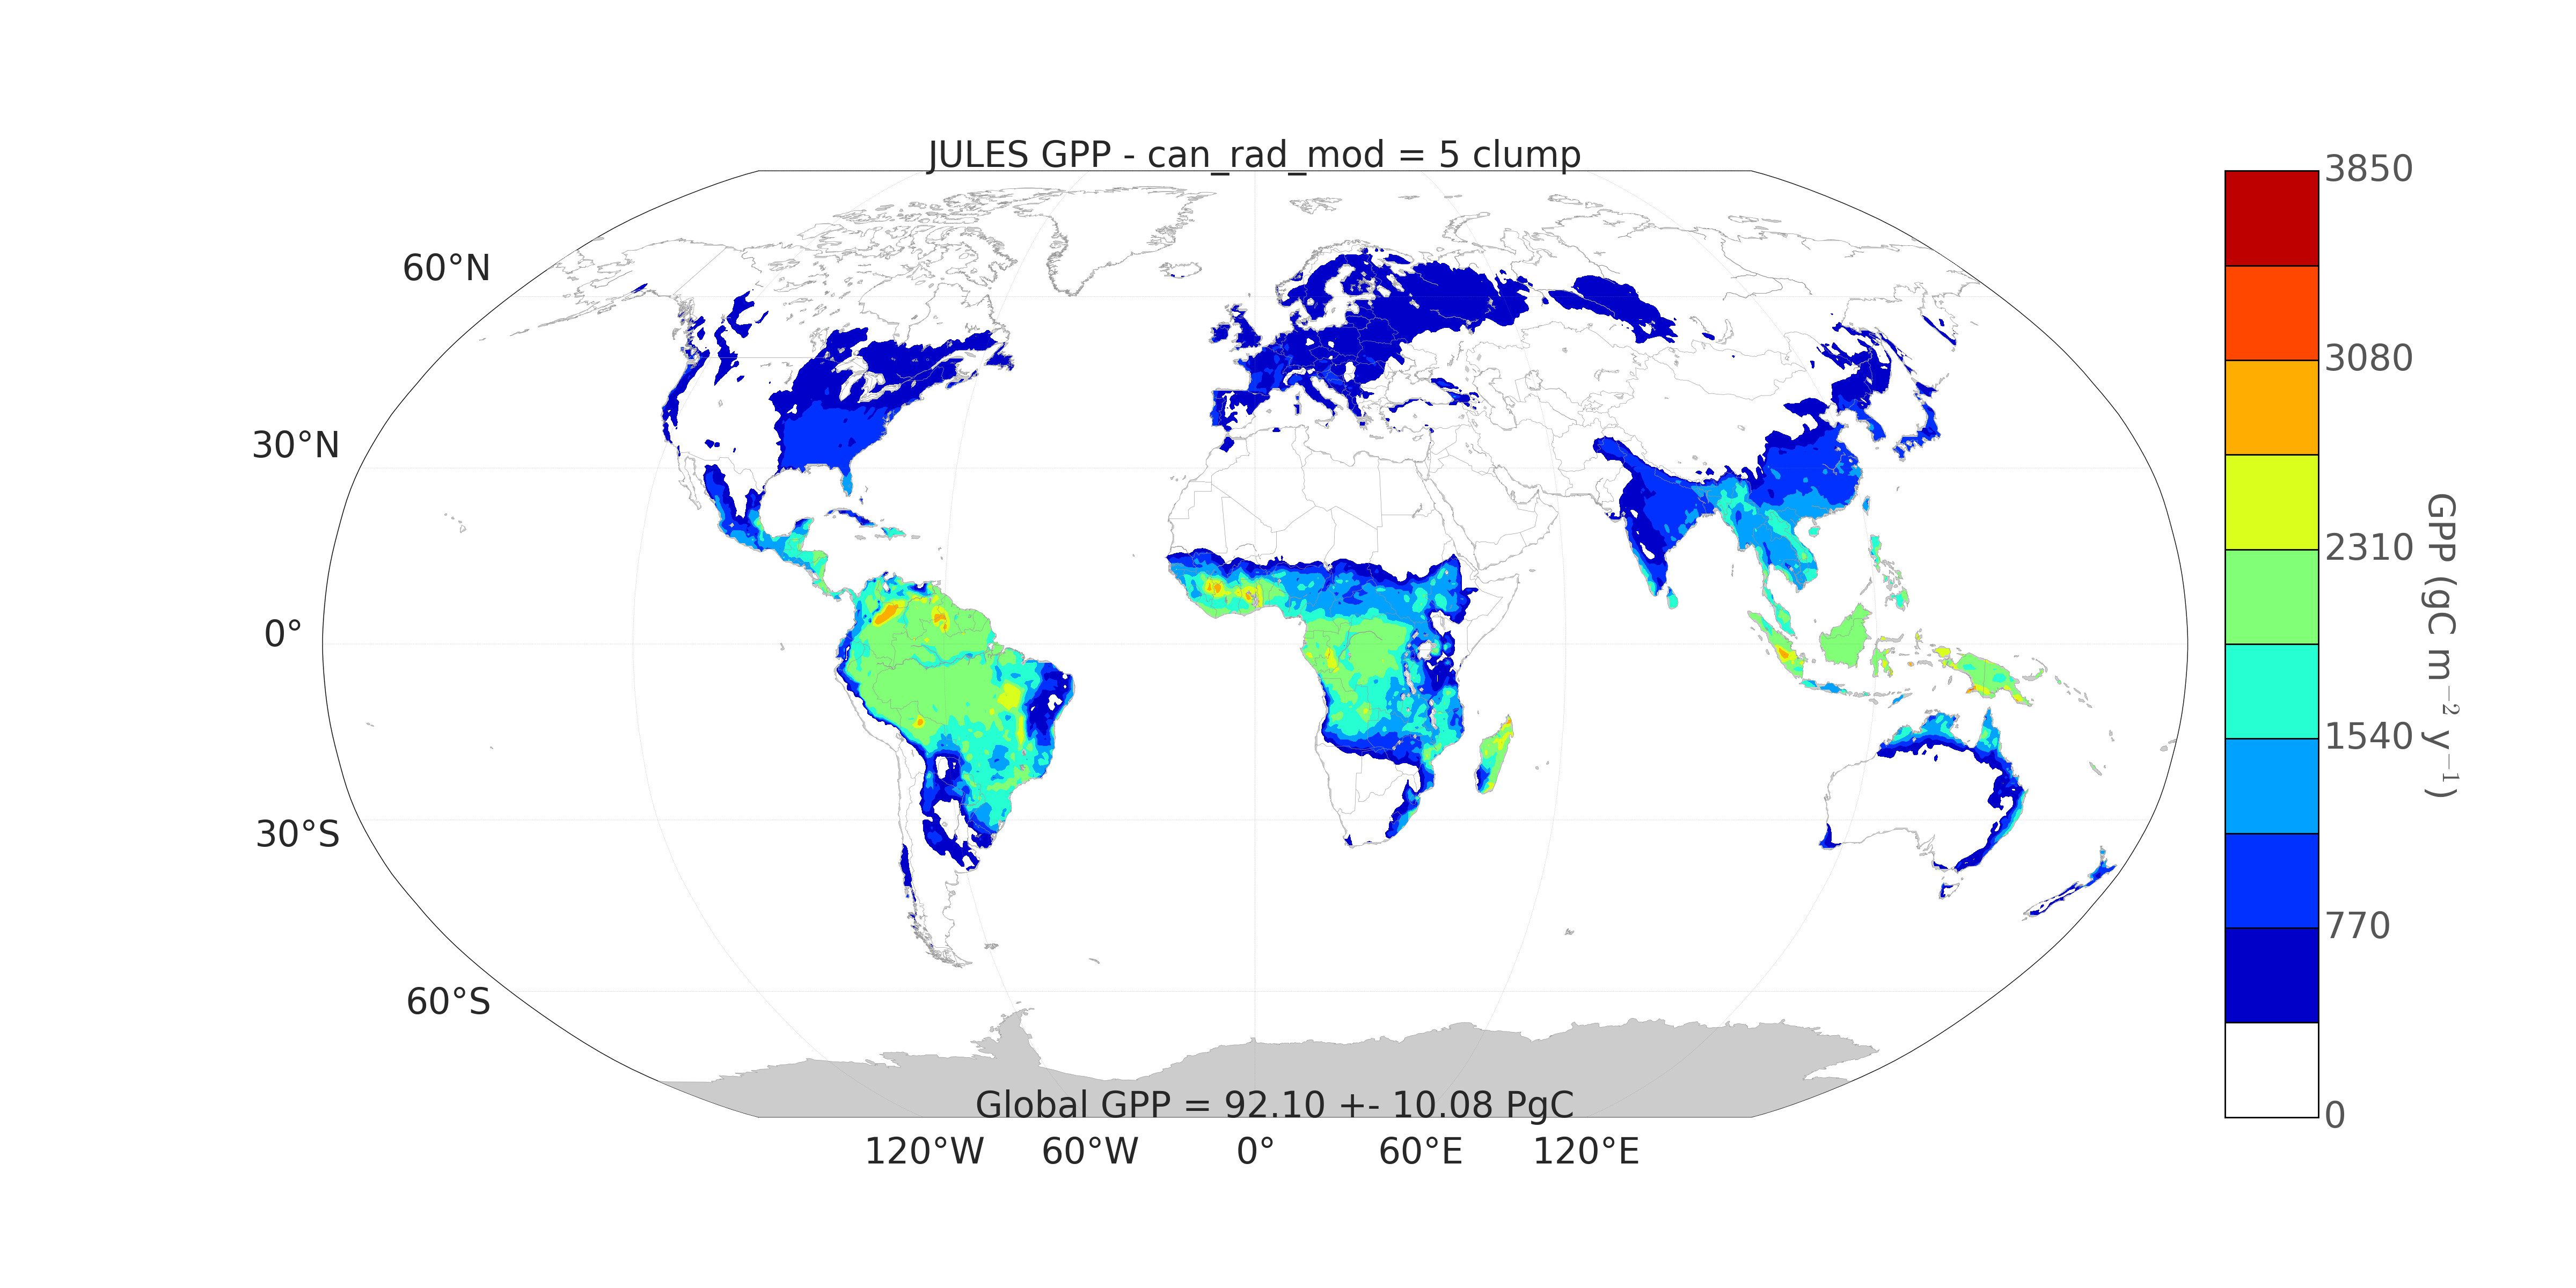
\includegraphics[width=0.5\textwidth]{/home/mn811042/Thesis/chapter6/figures_ofi/jules_opt5_clump_year.png}}
\end{tabular}
\begin{tabular}{ll}
\subfloat[Opt 4 - MTE]{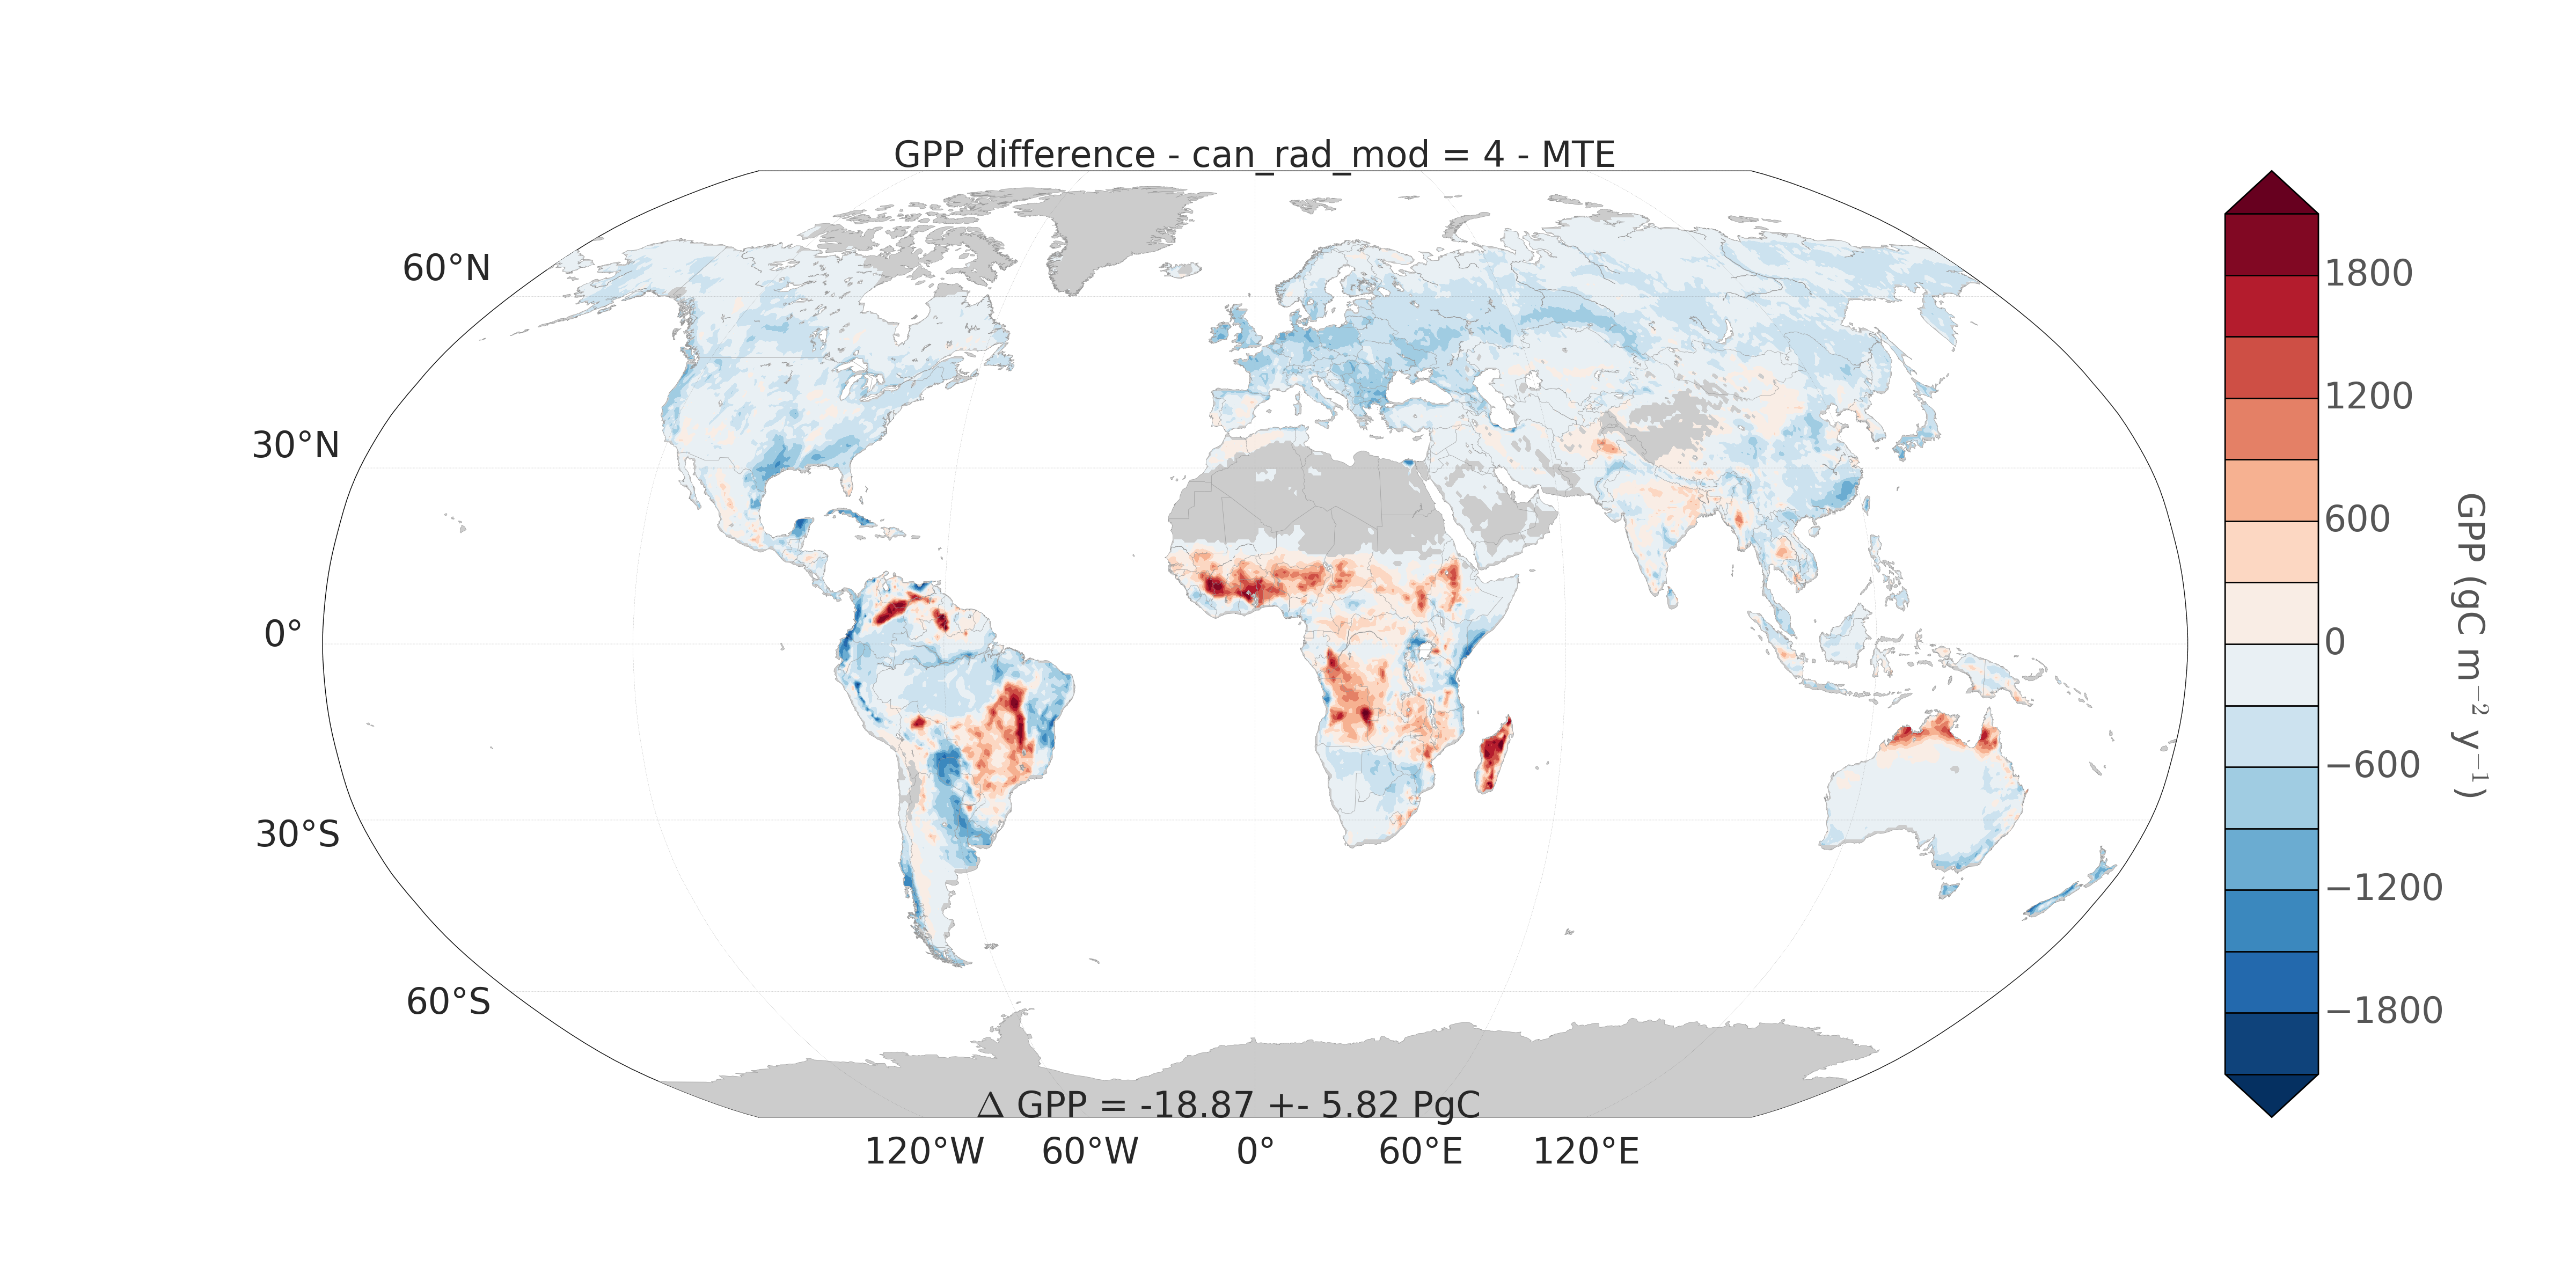
\includegraphics[width=0.5\textwidth]{/home/mn811042/Thesis/chapter6/figures_ofi/jules_diff_opt4_MTE_year.png}}
\subfloat[Opt 4 clump - MTE]{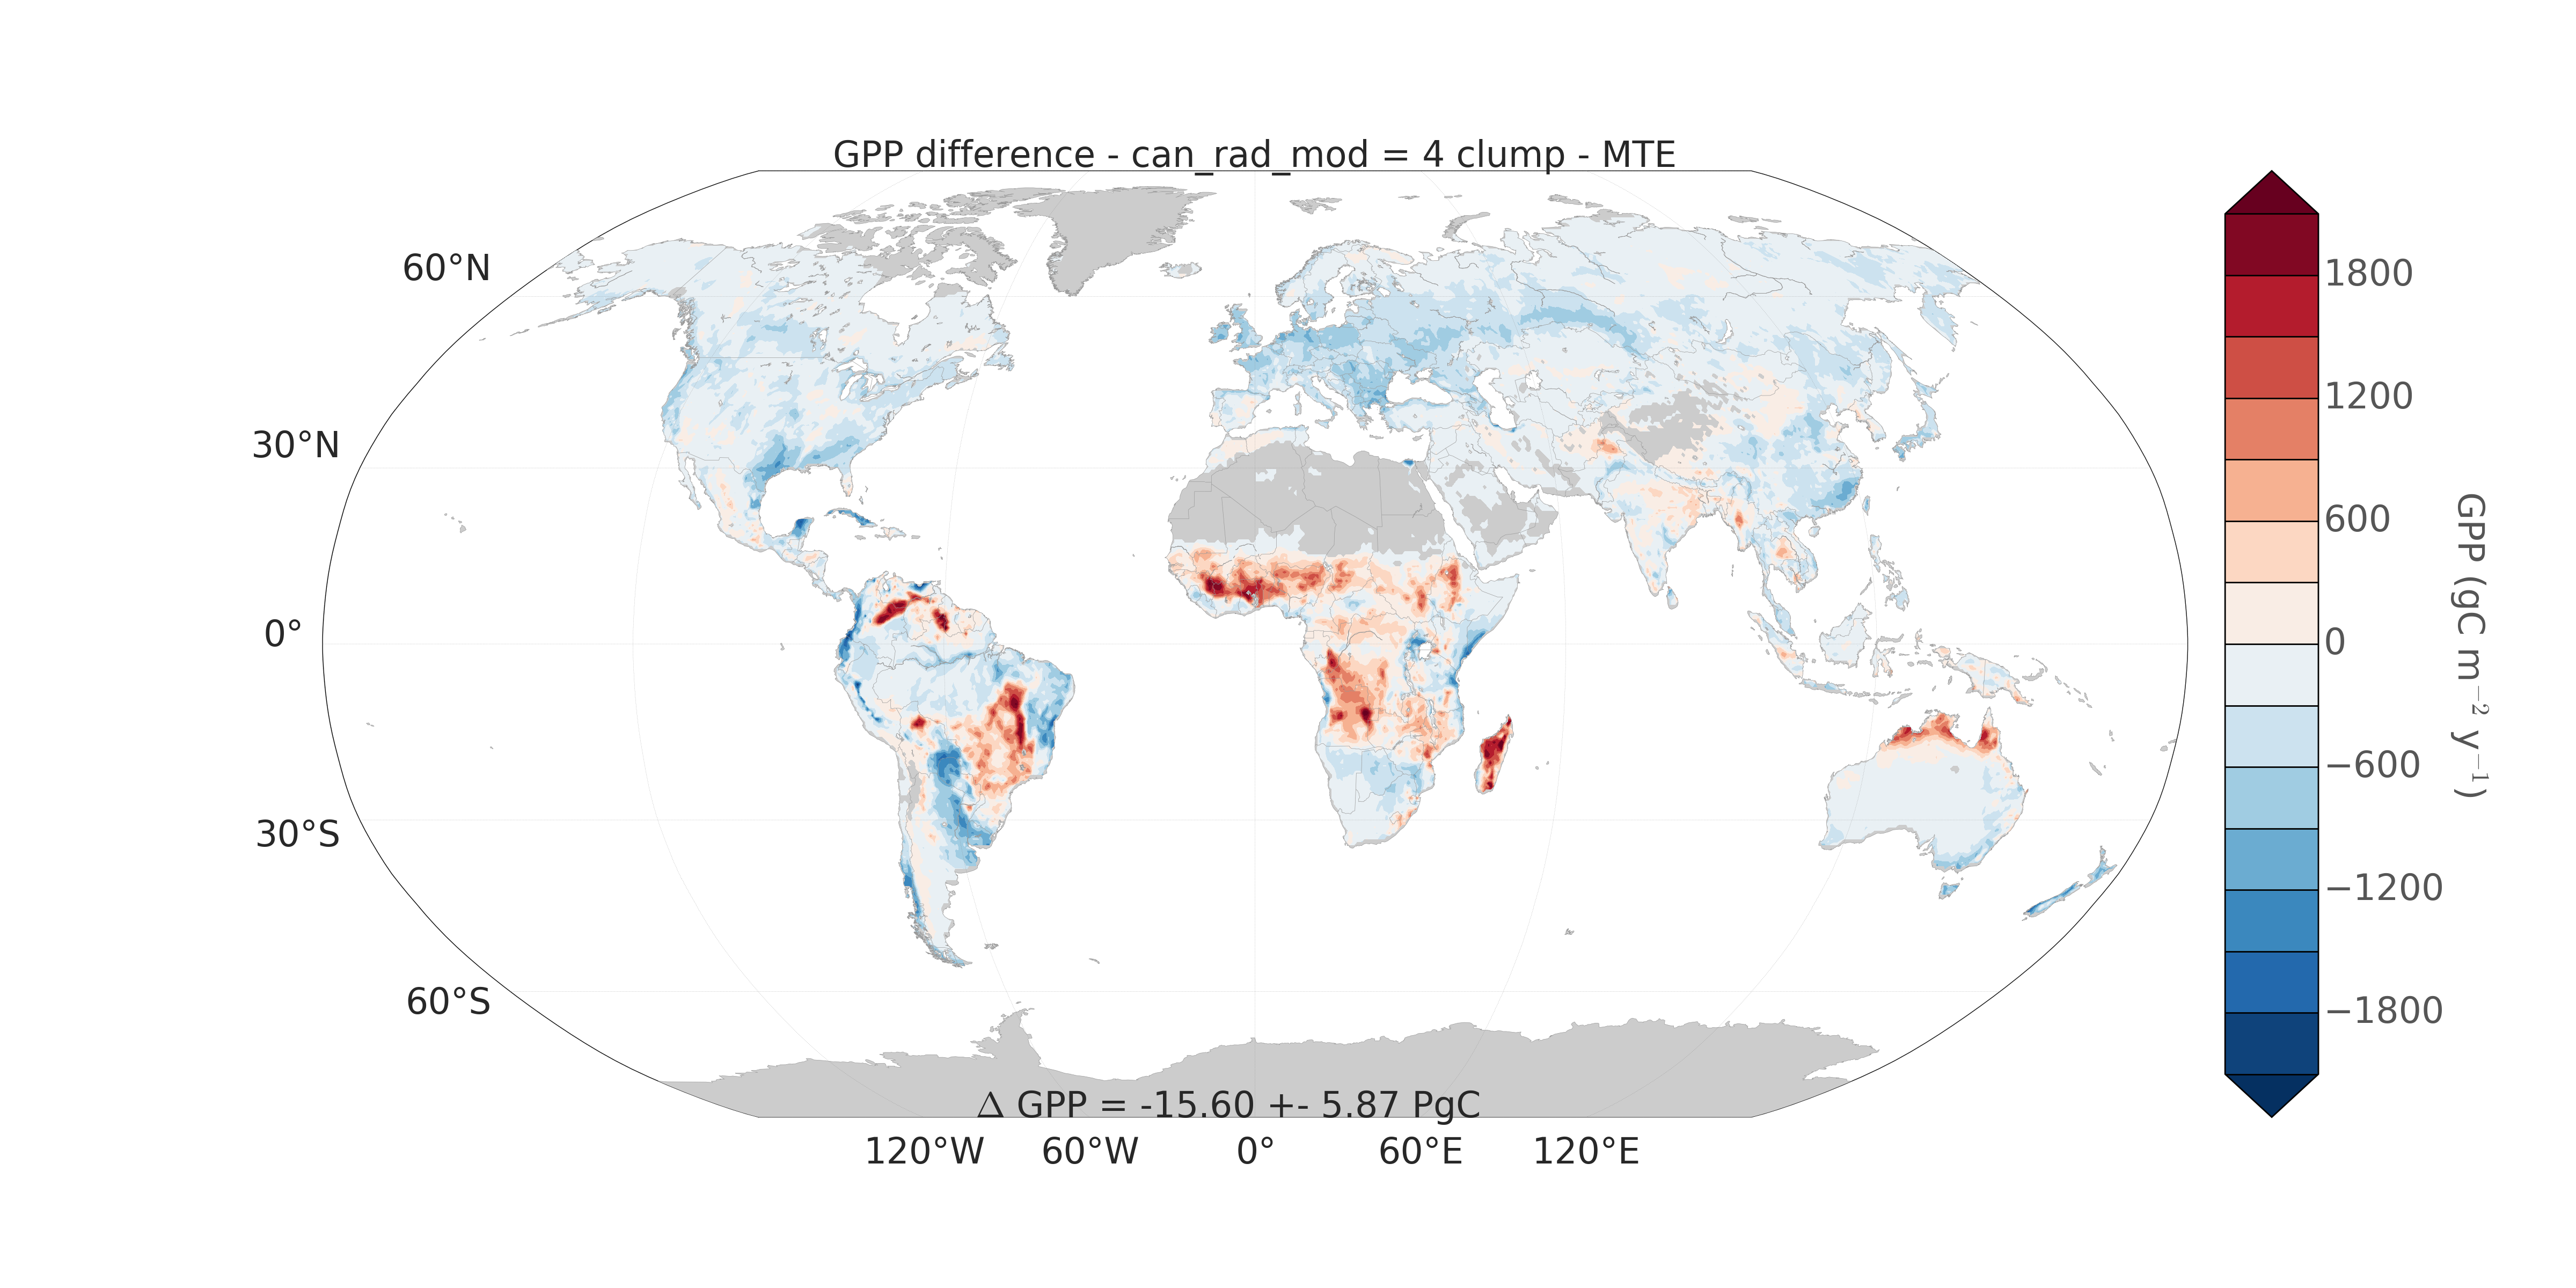
\includegraphics[width=0.5\textwidth]{/home/mn811042/Thesis/chapter6/figures_ofi/jules_diff_opt4_clump_MTE_year.png}}
\end{tabular}
\begin{tabular}{ll}
\subfloat[Opt 5 - MTE]{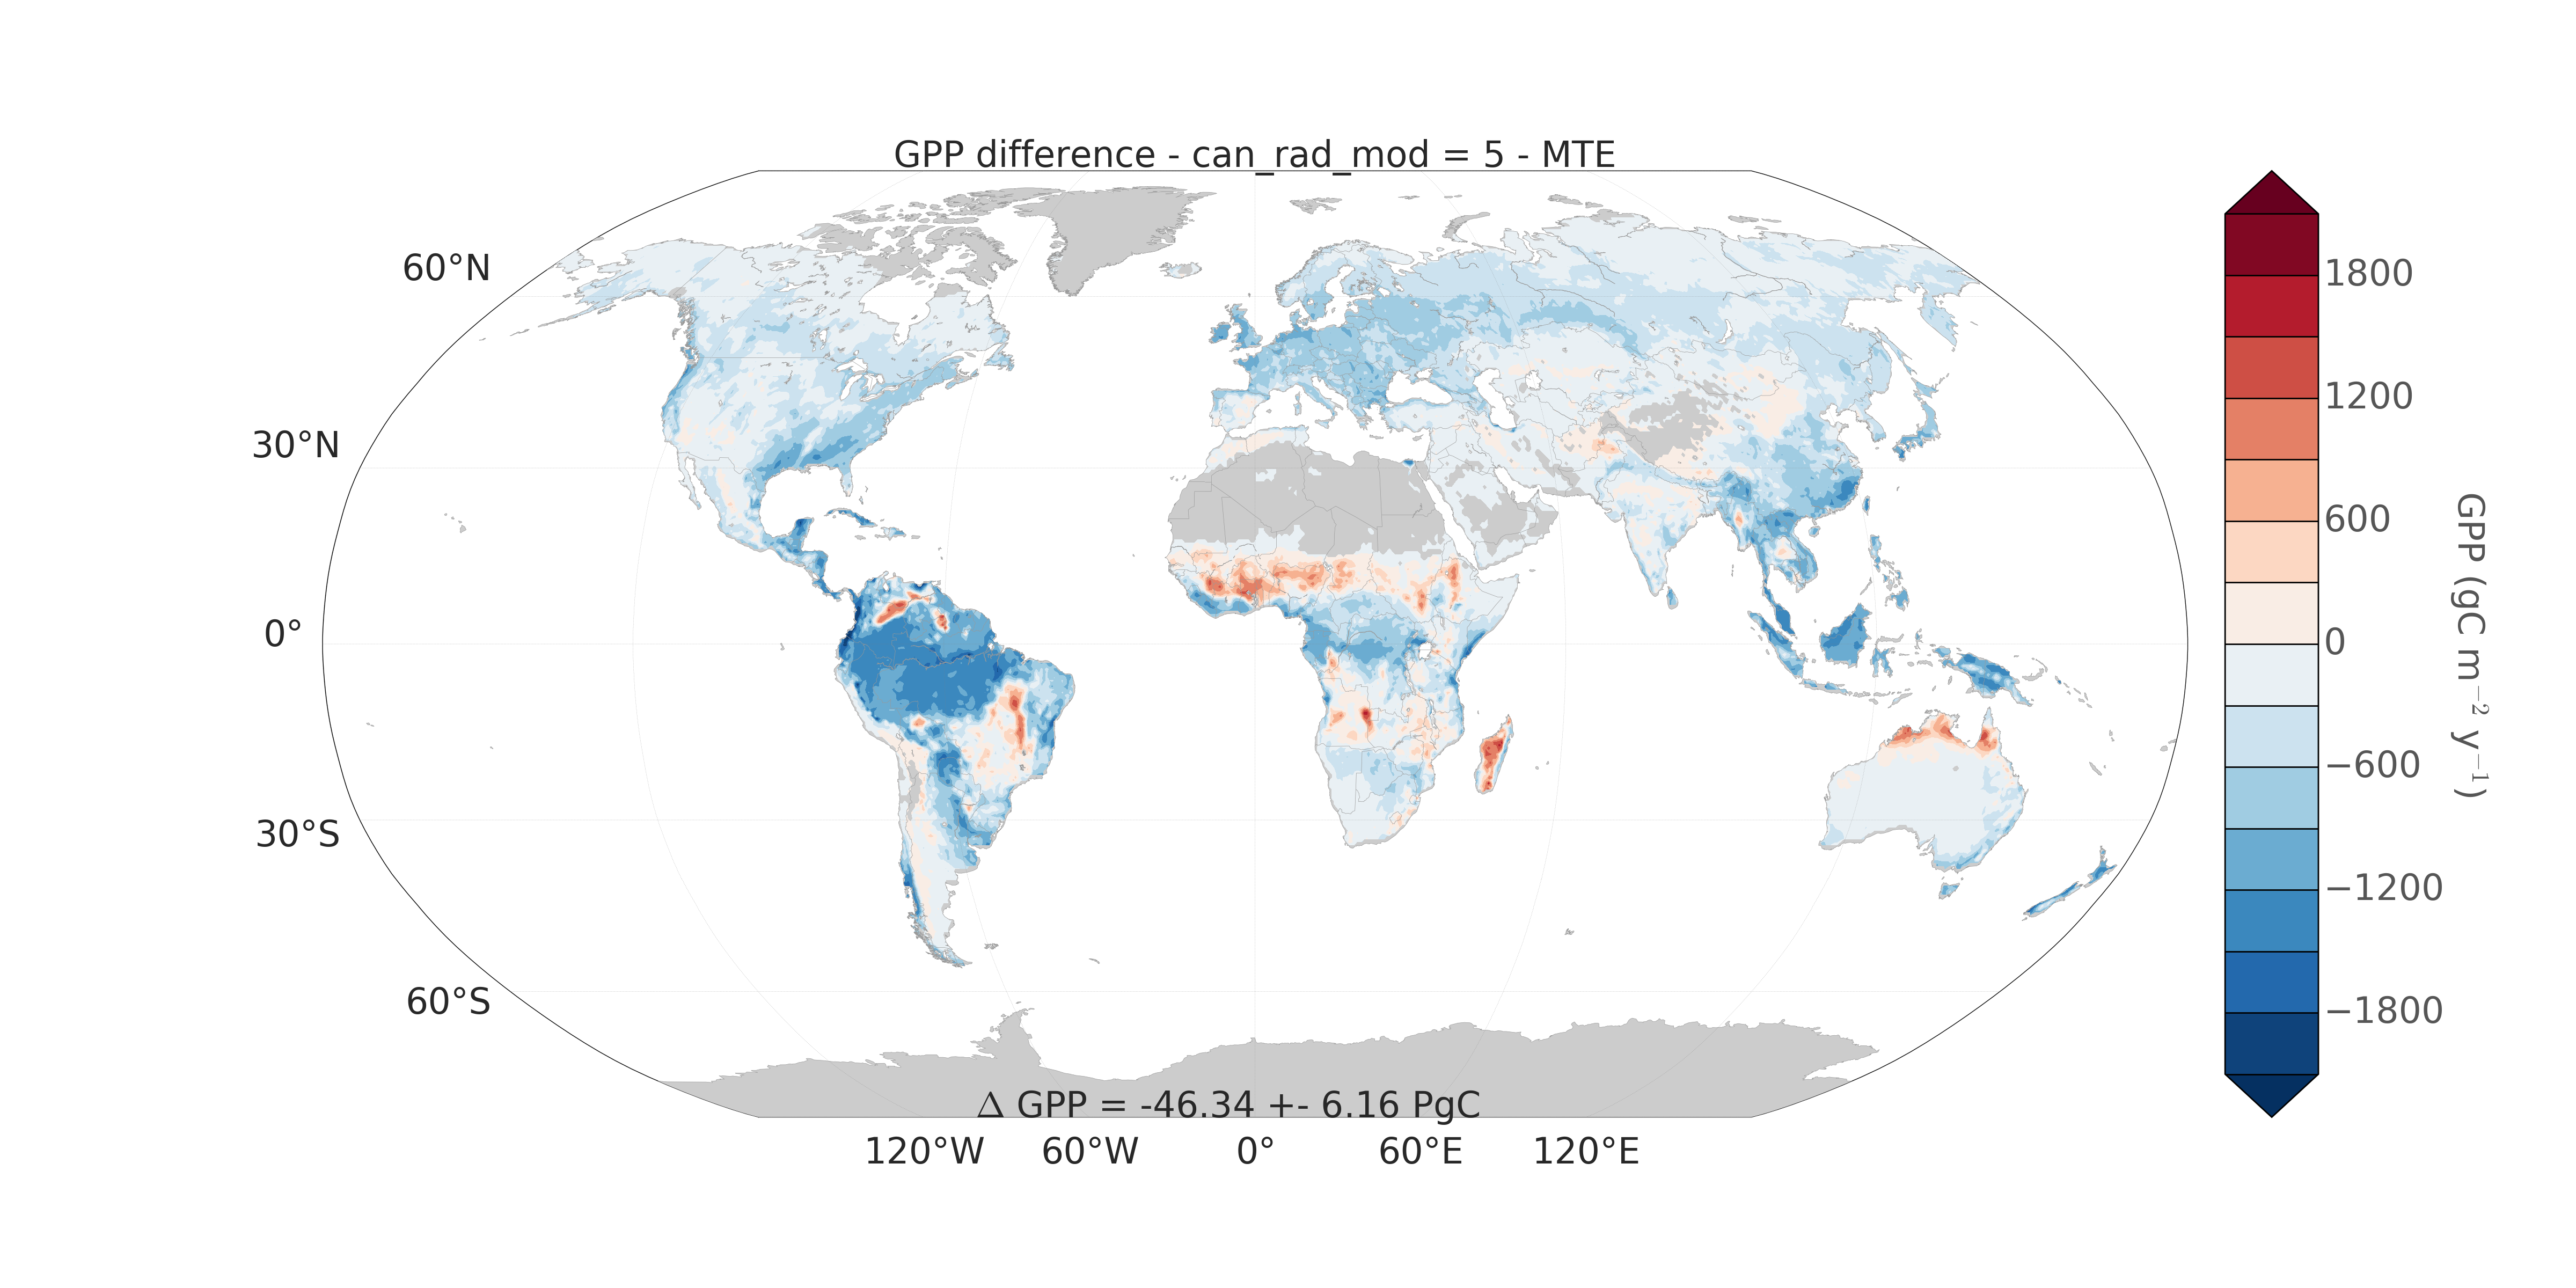
\includegraphics[width=0.5\textwidth]{/home/mn811042/Thesis/chapter6/figures_ofi/jules_diff_opt5_MTE_year.png}}
\subfloat[Opt 5 clump - MTE]{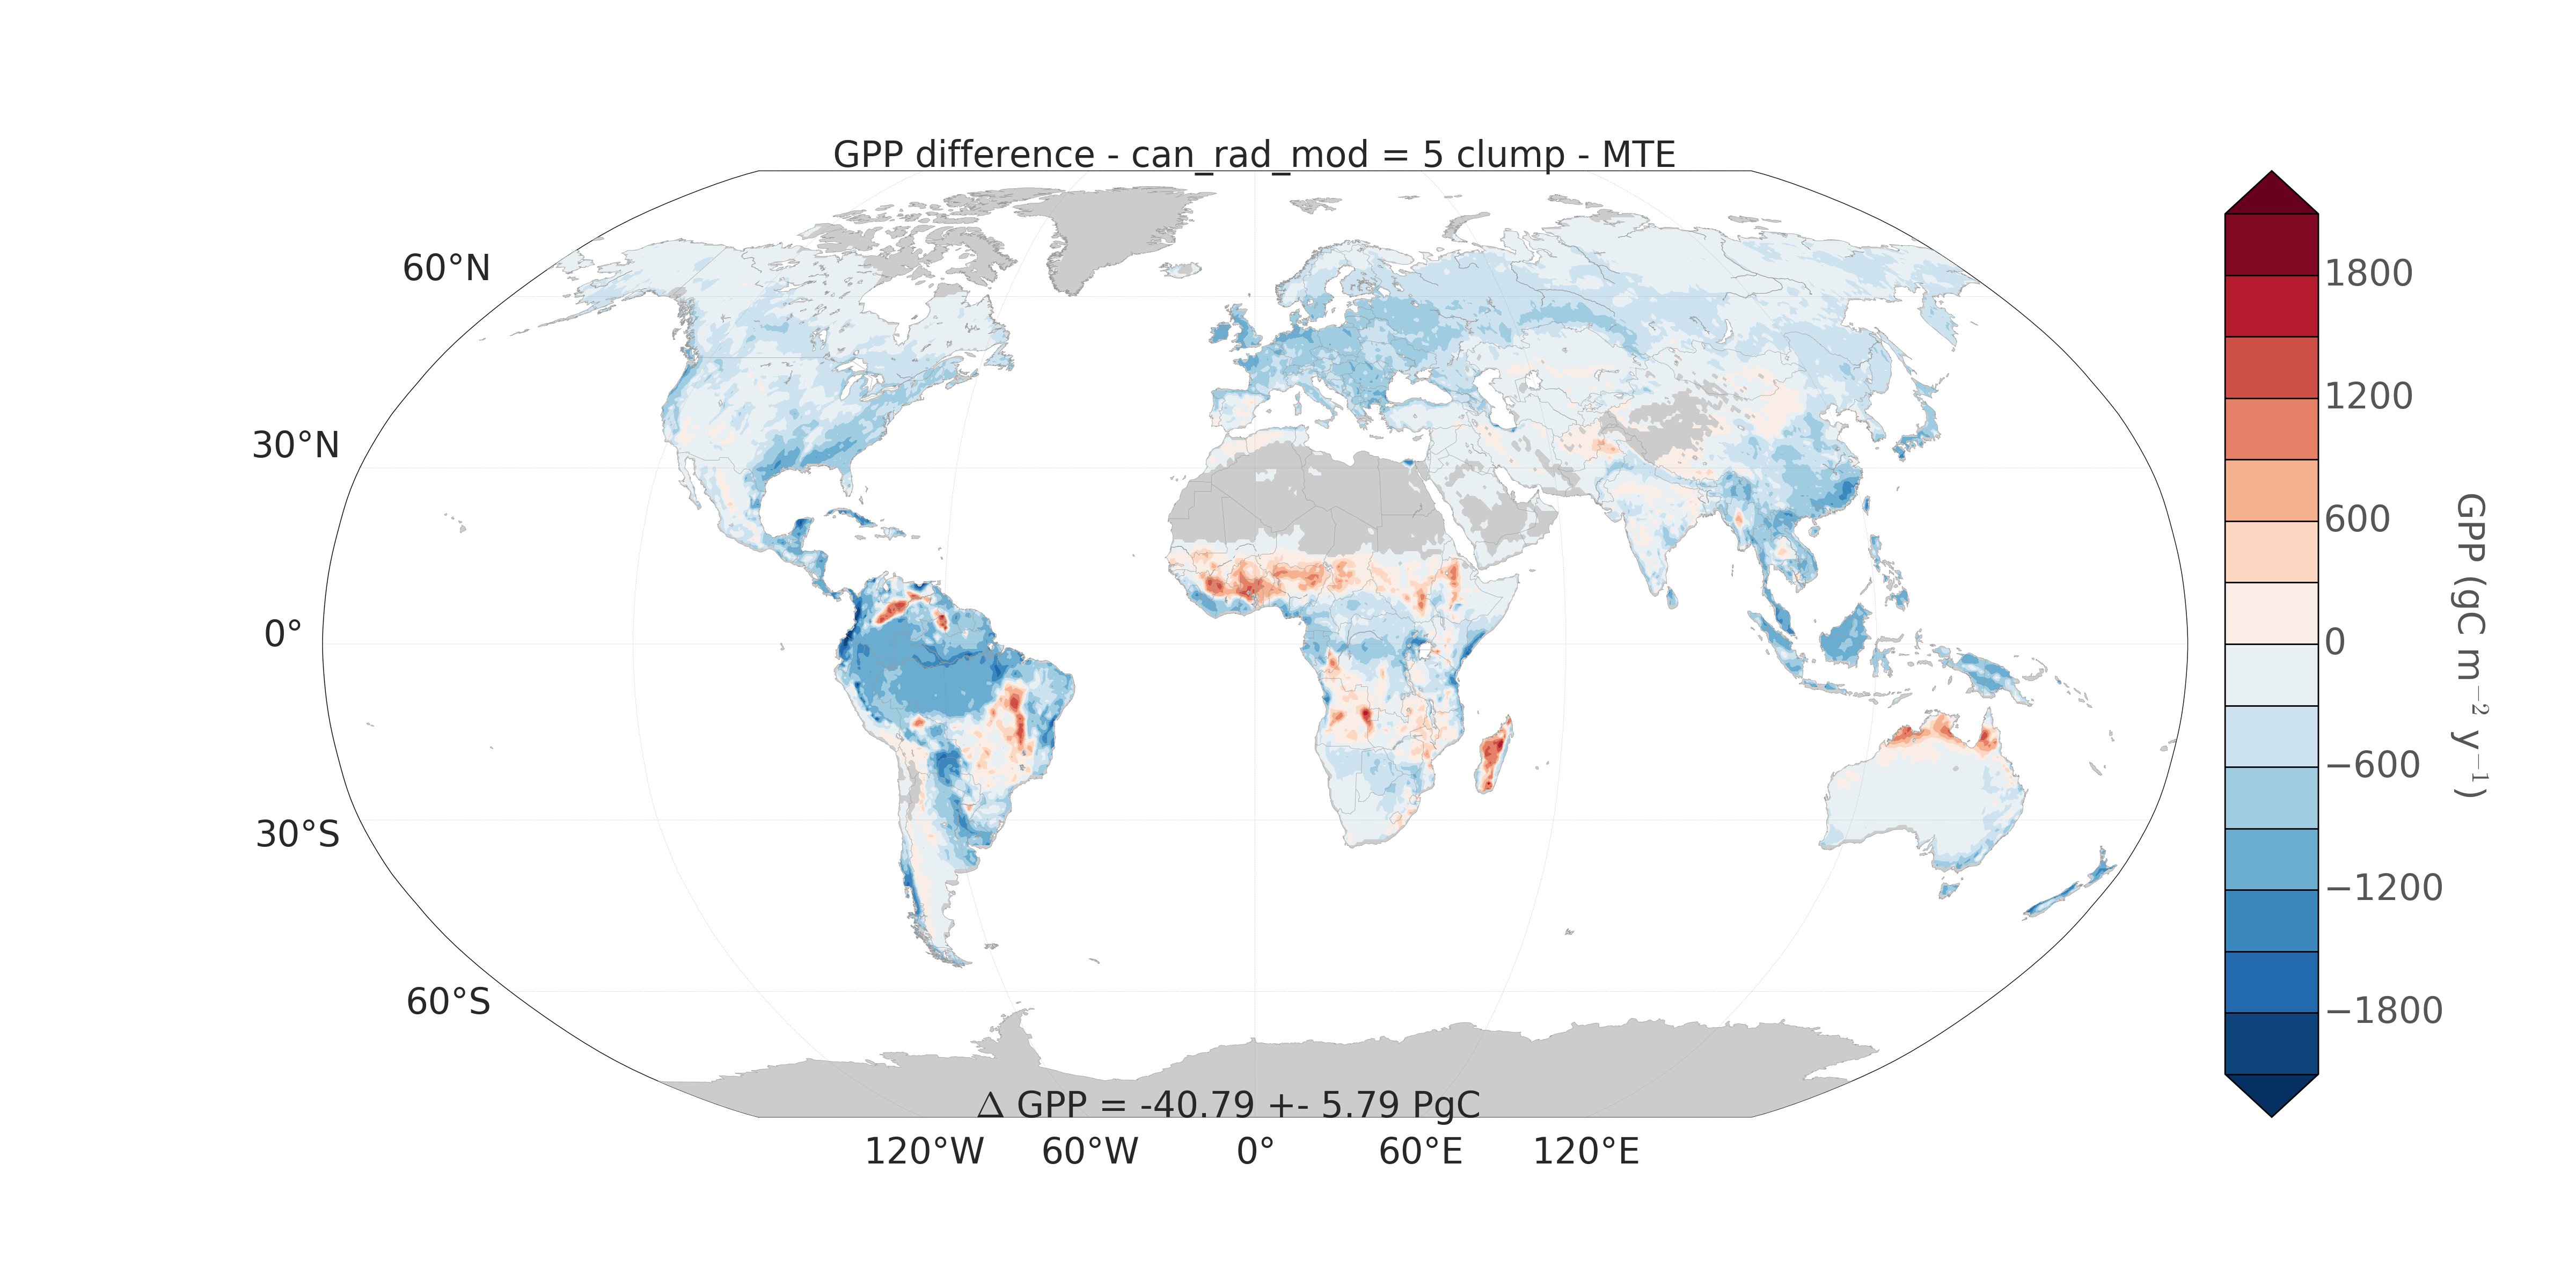
\includegraphics[width=0.5\textwidth]{/home/mn811042/Thesis/chapter6/figures_ofi/jules_diff_opt5_clump_MTE_year.png}}
\end{tabular}
\caption{Total average GPP for the year of 2008.} 
\label{f:pgap}
\end{figure}


\begin{figure}[ht!]
\centering
\begin{tabular}{ll}
\subfloat[Opt 4 - clump]{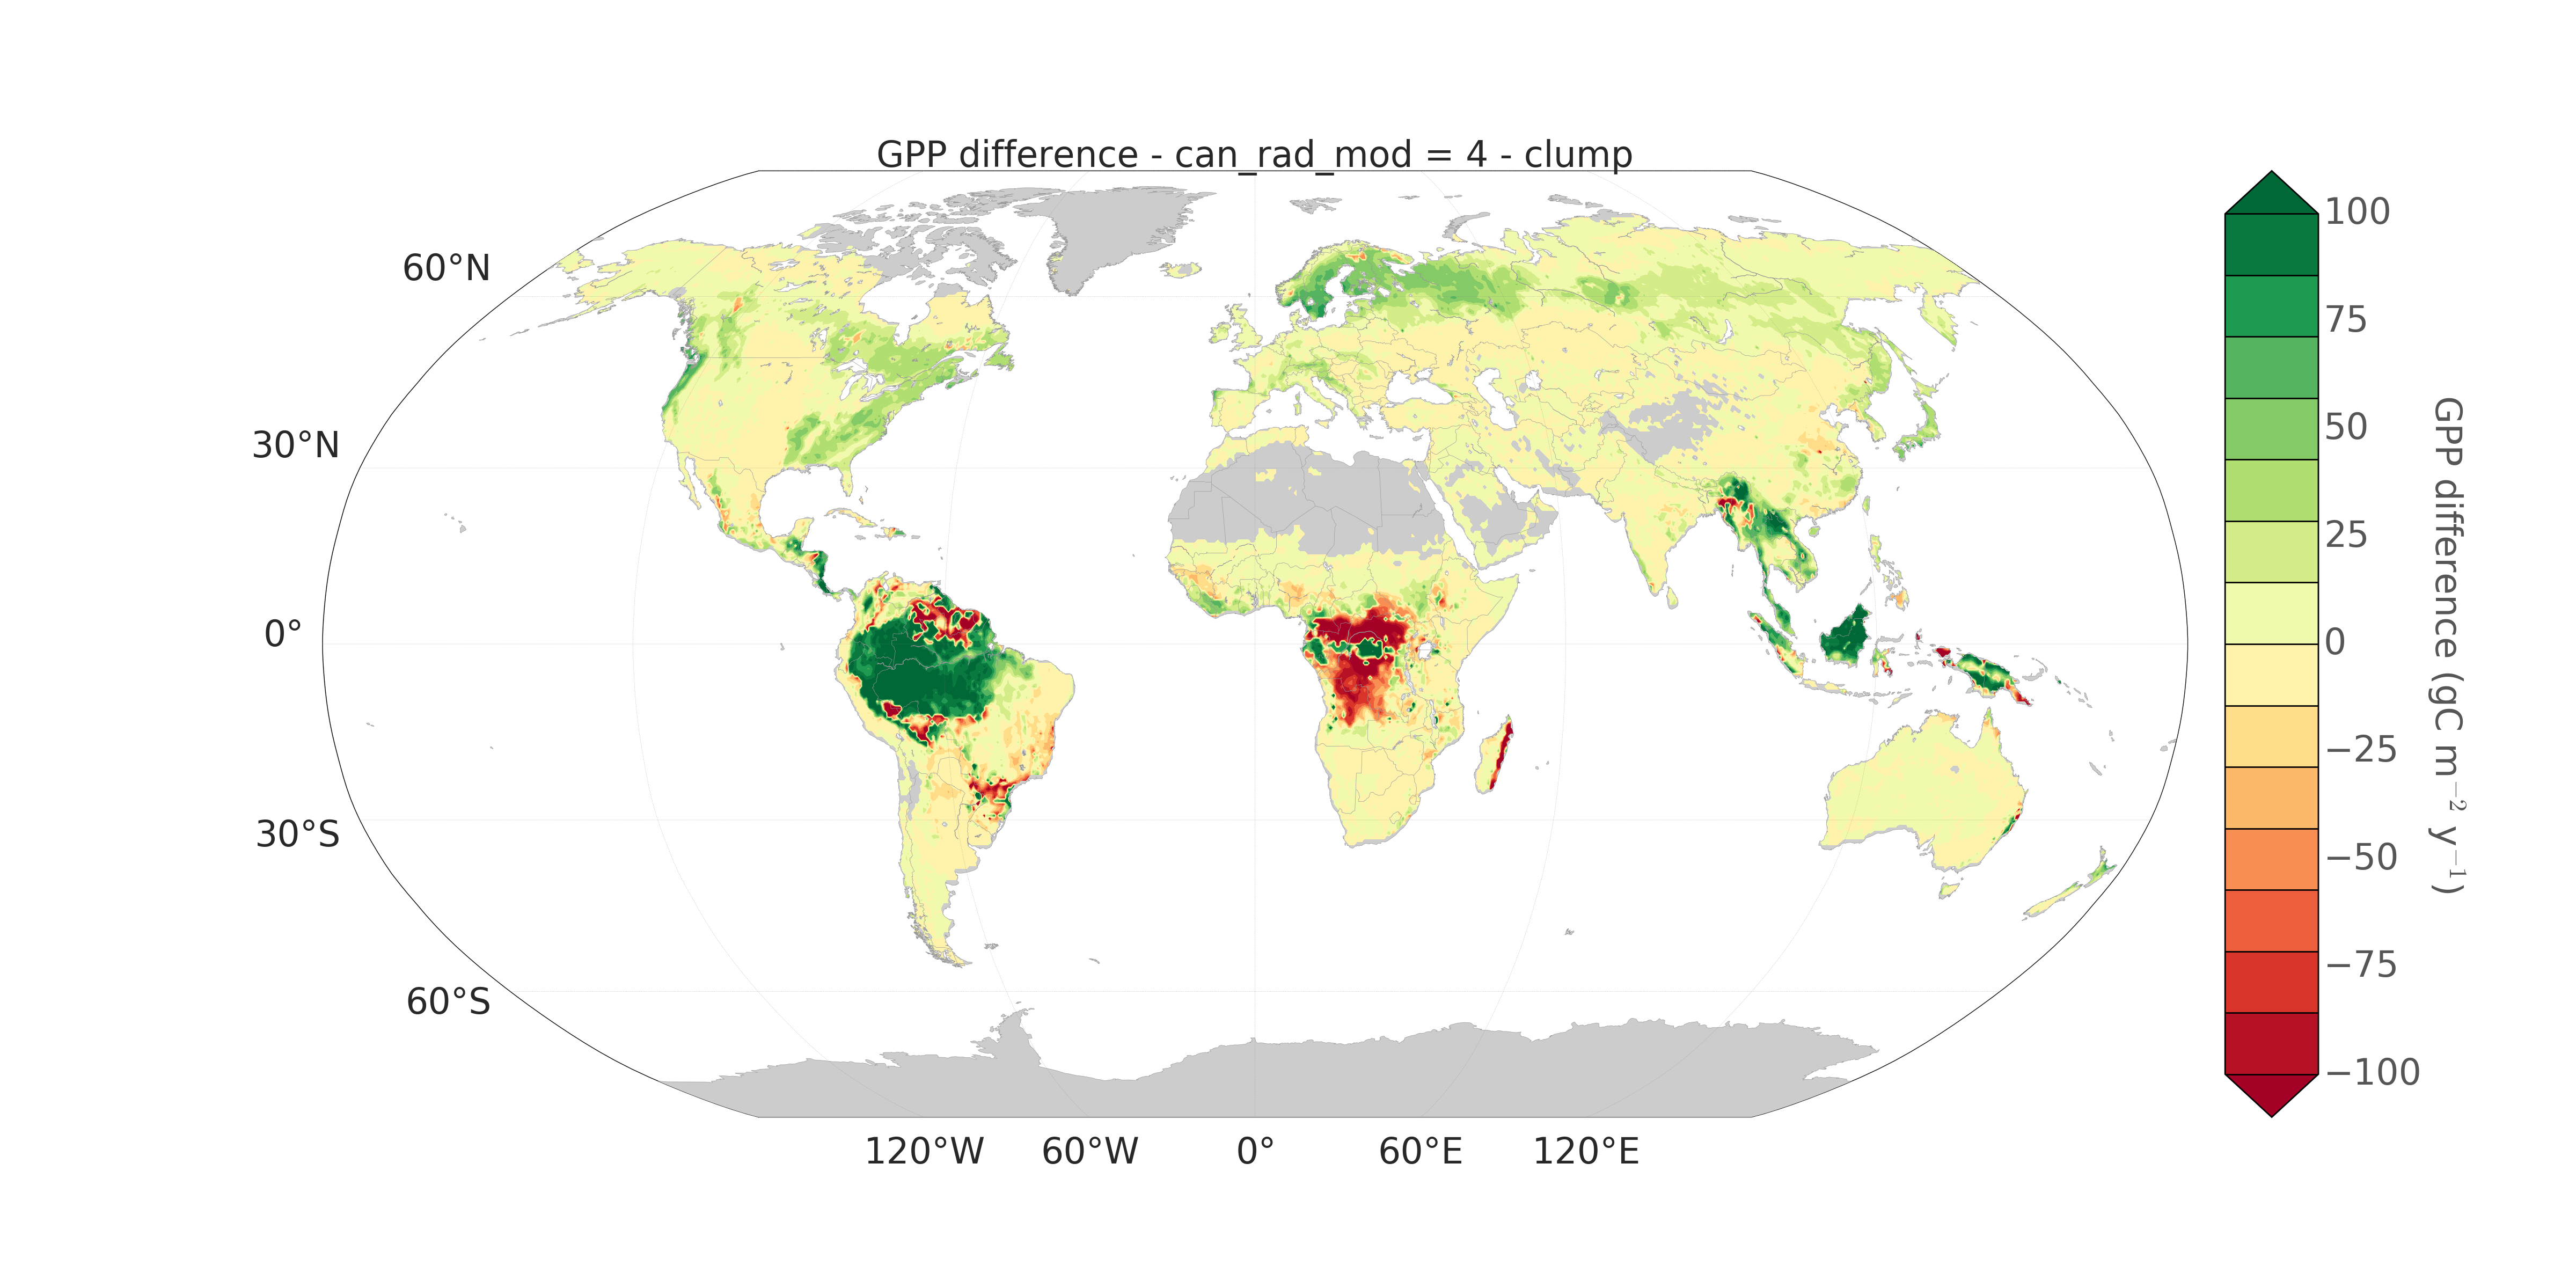
\includegraphics[width=0.5\textwidth]{/home/mn811042/Thesis/chapter6/figures_ofi/jules_improve_opt4_clump_MTE_year.png}}
\subfloat[Opt 5 - clump]{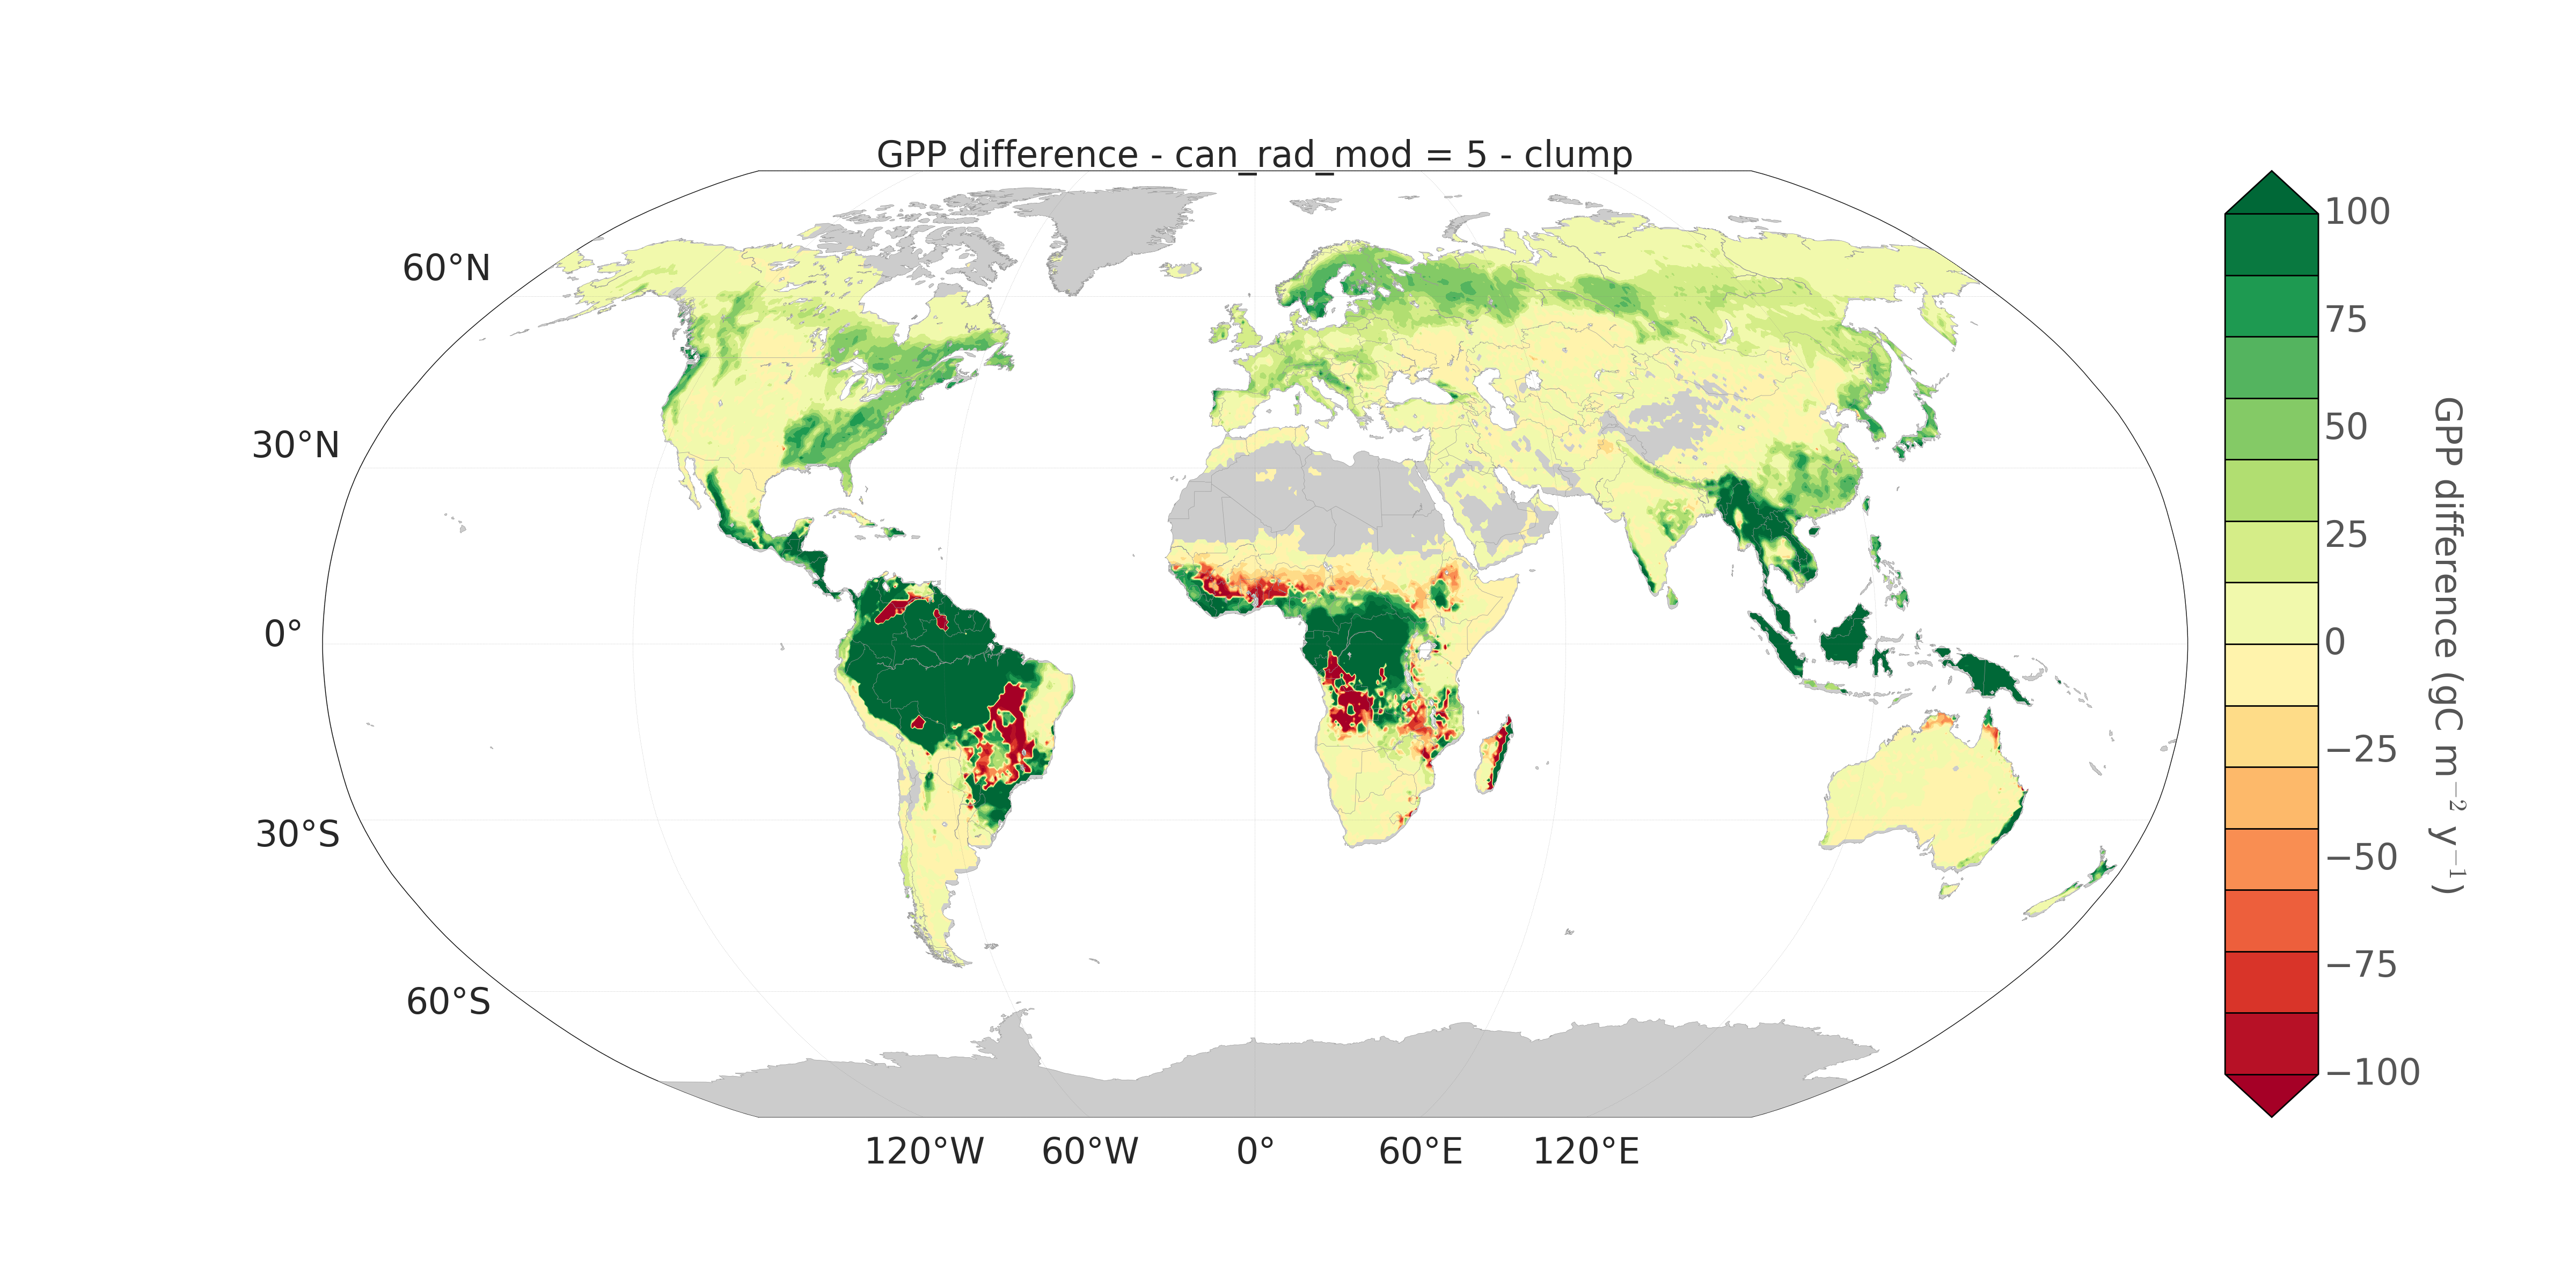
\includegraphics[width=0.5\textwidth]{/home/mn811042/Thesis/chapter6/figures_ofi/jules_improve_opt5_clump_MTE_year.png}}
\end{tabular}
\begin{tabular}{l}
\subfloat[GL4.0 - Opt 5 - clump]{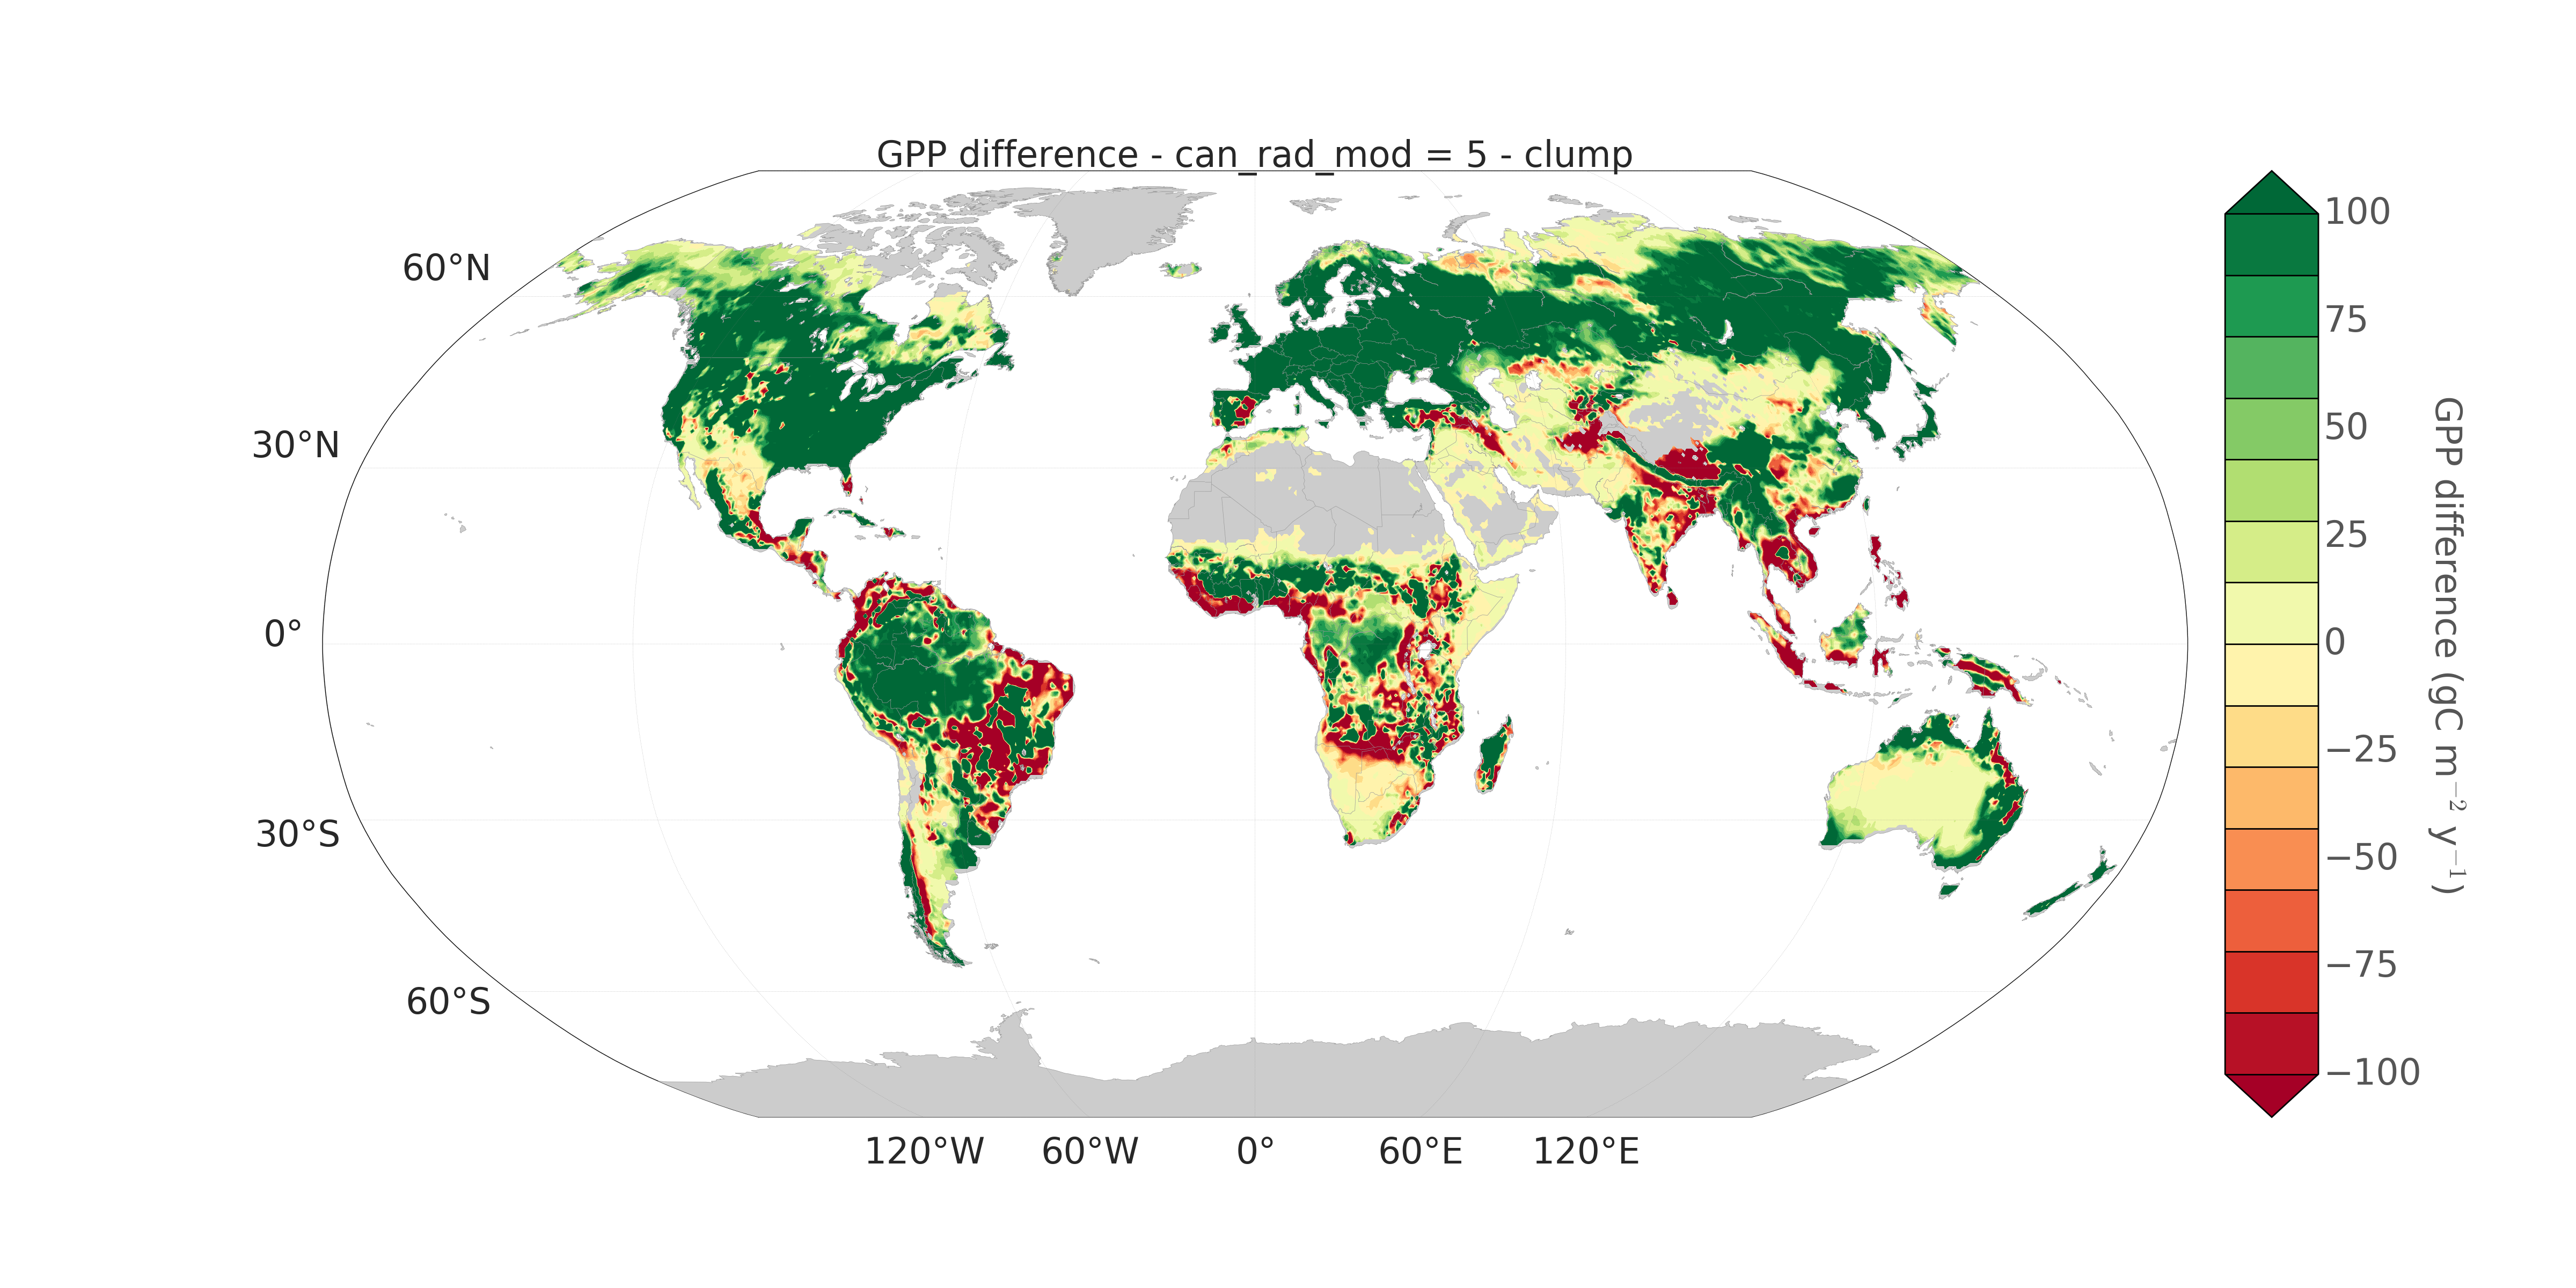
\includegraphics[width=1.0\textwidth]{/home/mn811042/Thesis/chapter6/figures_ofi/jules_improve_GL4_opt5_clump_MTE_year.png}}
\end{tabular}


\caption{Green areas represent more agreement with the MTE dataset by considering clumping.} 
\label{f:improve}
\end{figure}

The red areas on Figure~\ref{f:improve}b are related to a higher presence of C4 plants over South America and Africa, and with a minor impact over Australia. 


\begin{figure}[ht!]
\centering
\begin{tabular}{ll}
\subfloat[BL]{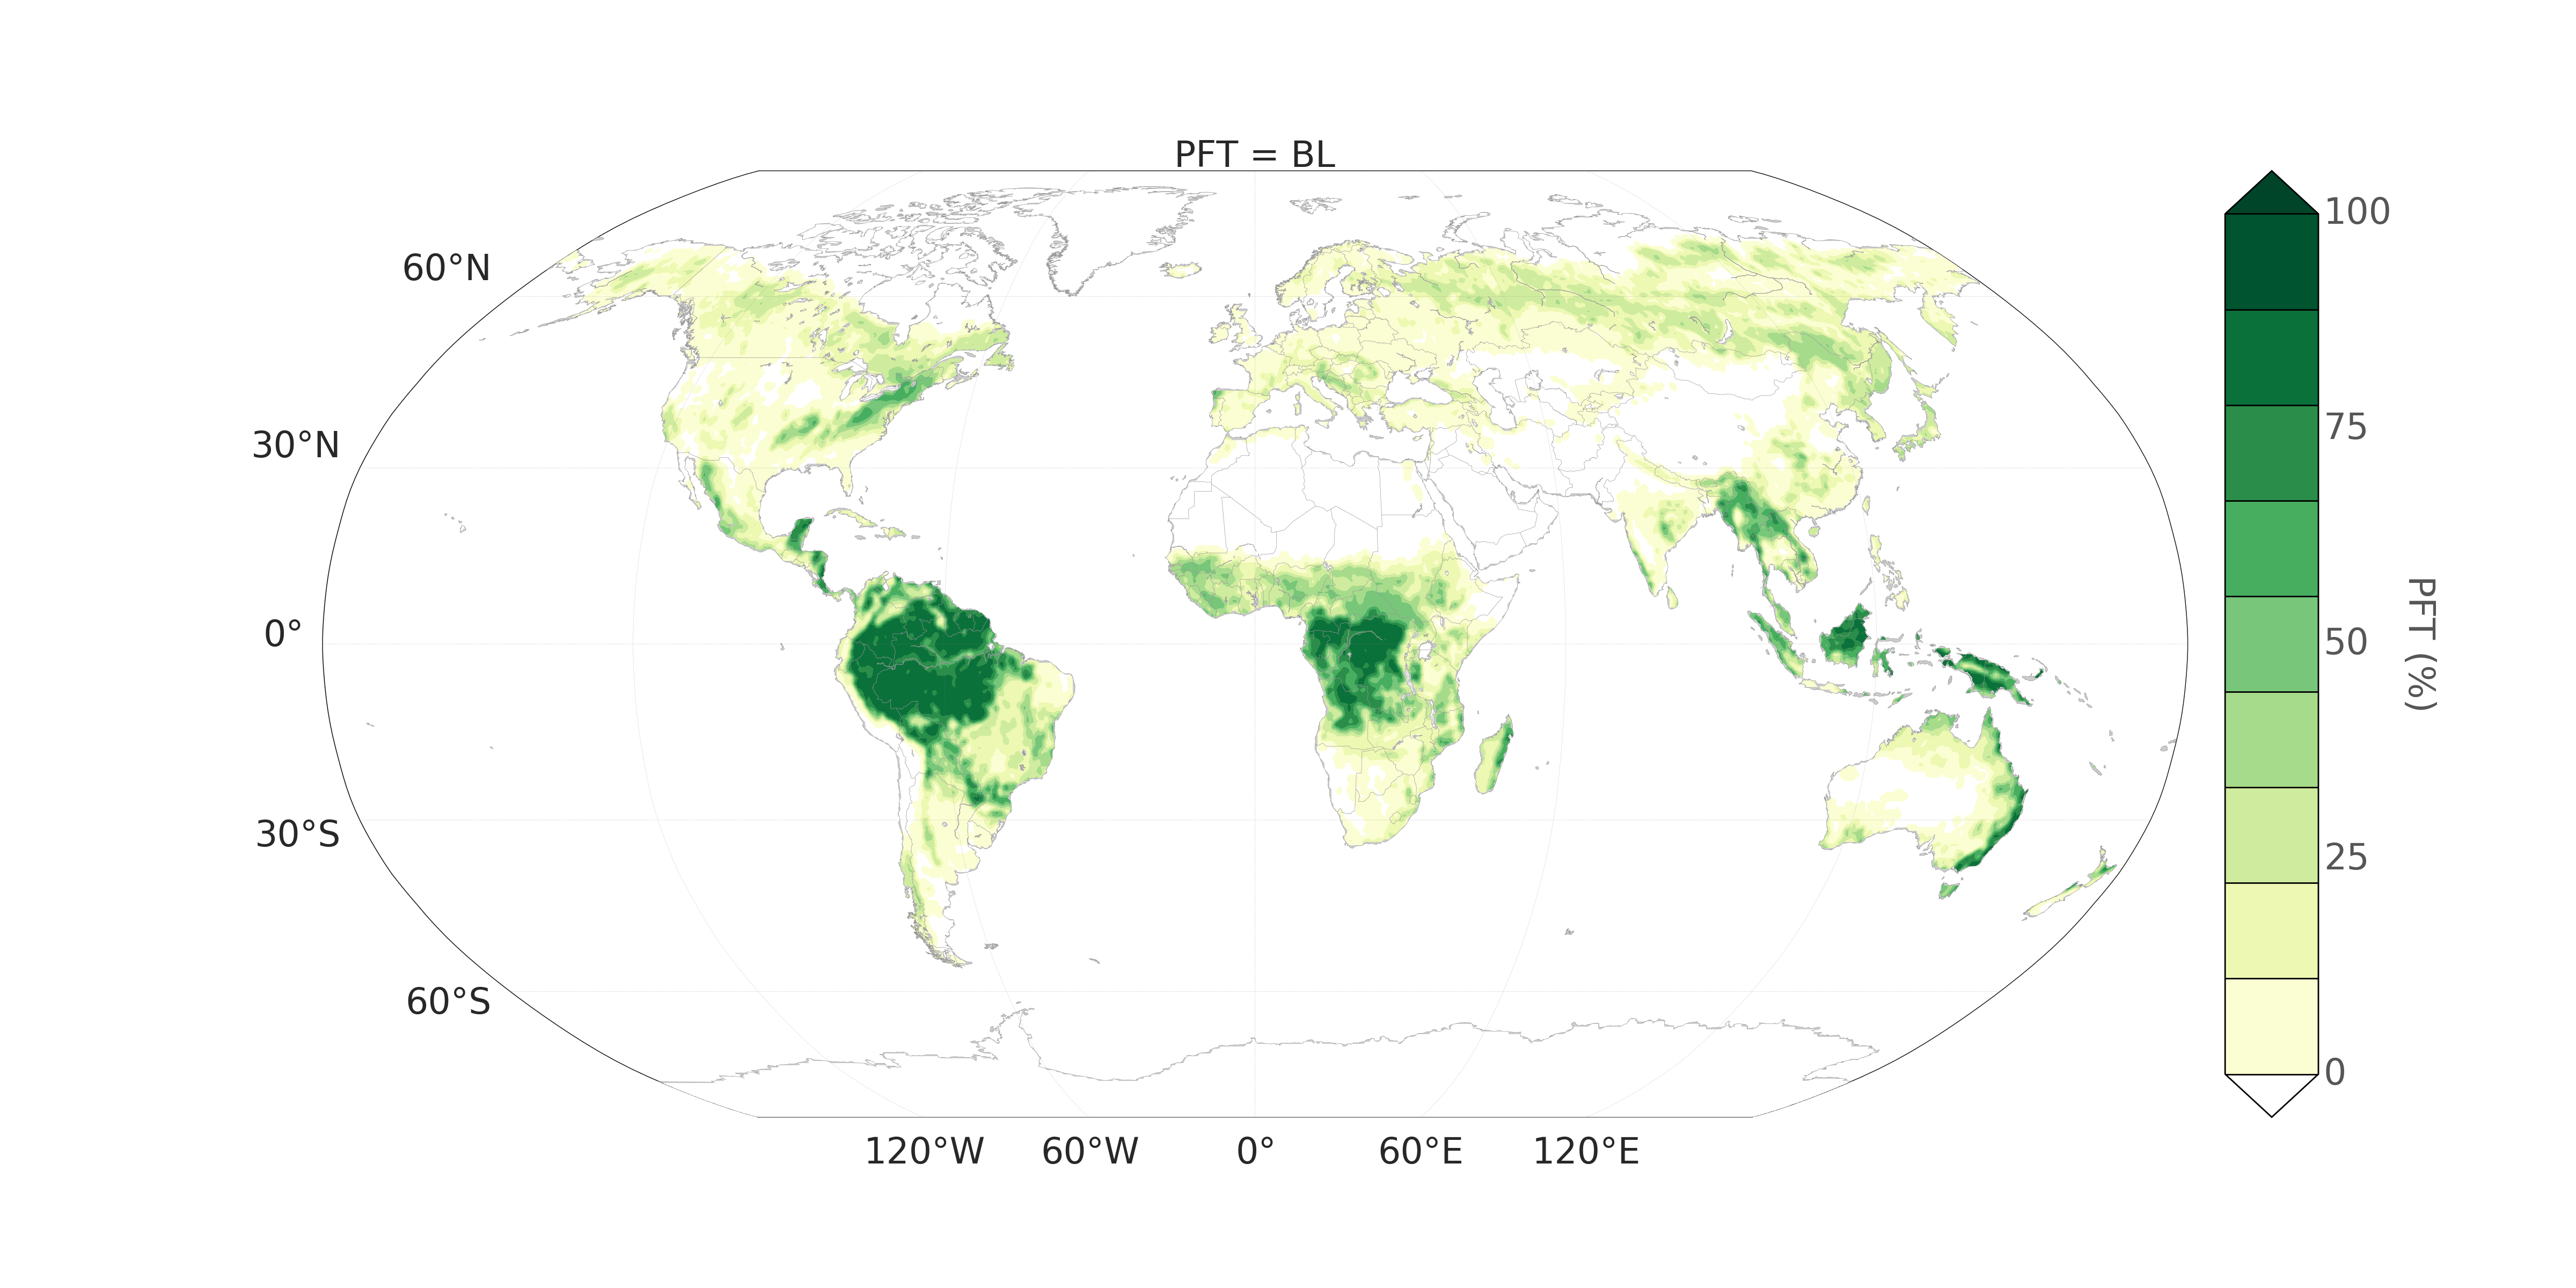
\includegraphics[width=0.5\textwidth]{/home/mn811042/Thesis/chapter6/figures_ofi/PFT_0.png}}
\subfloat[NL]{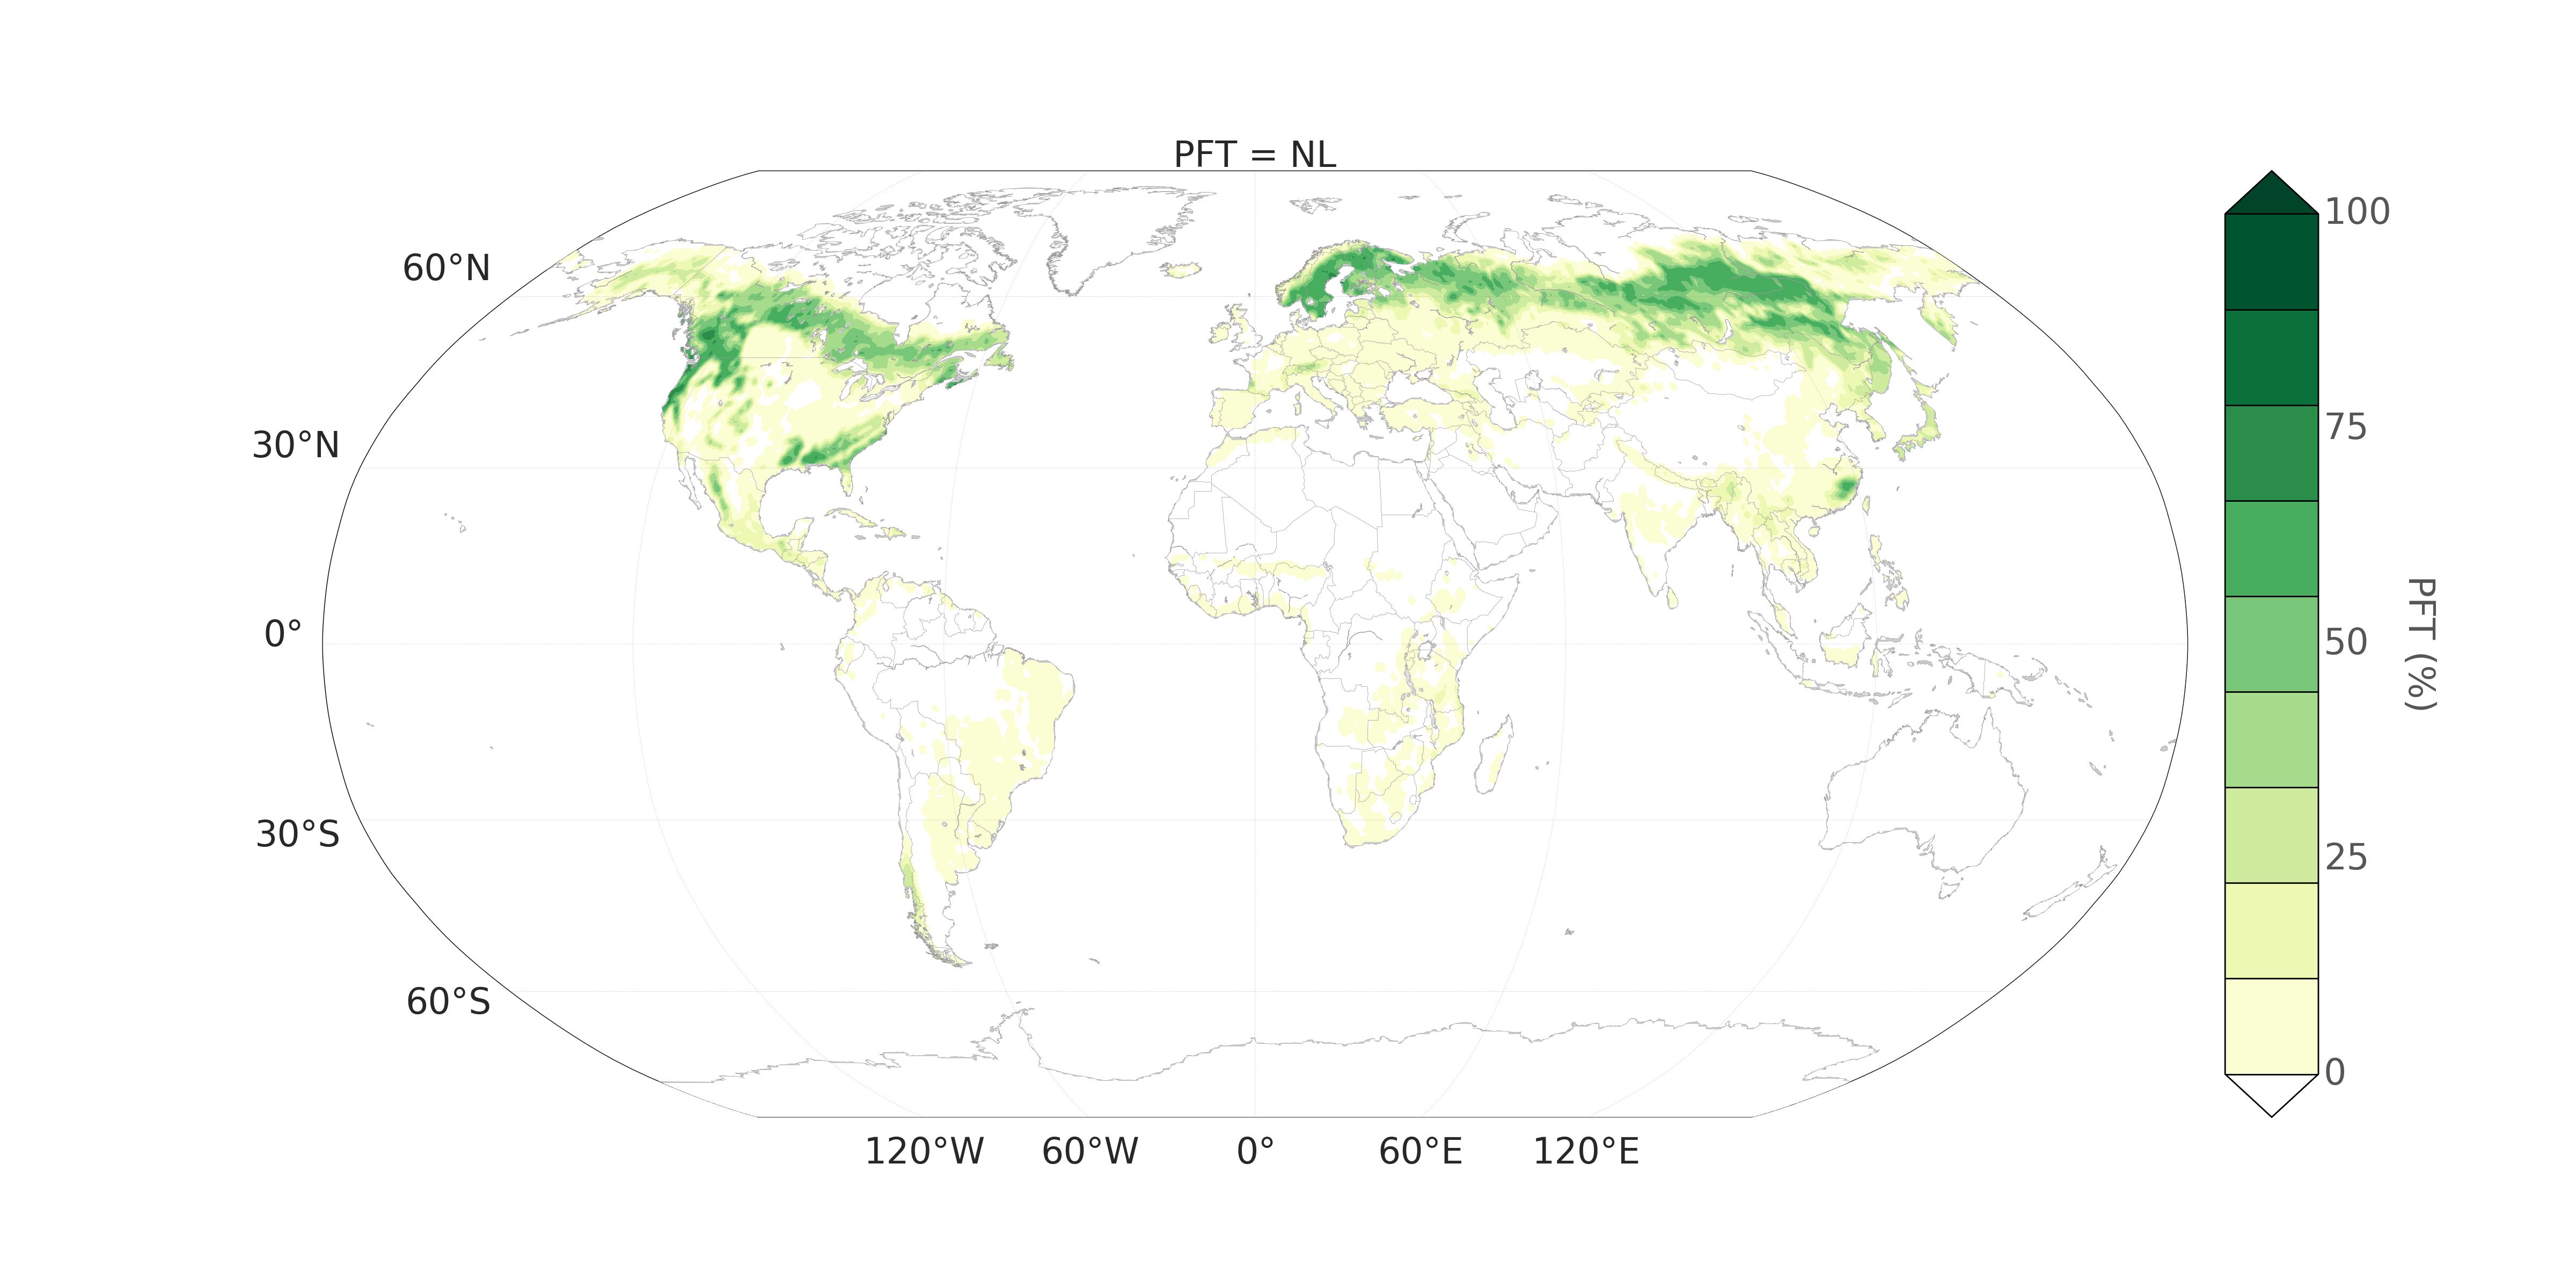
\includegraphics[width=0.5\textwidth]{/home/mn811042/Thesis/chapter6/figures_ofi/PFT_1.png}}
\end{tabular}
\begin{tabular}{ll}
\subfloat[C3]{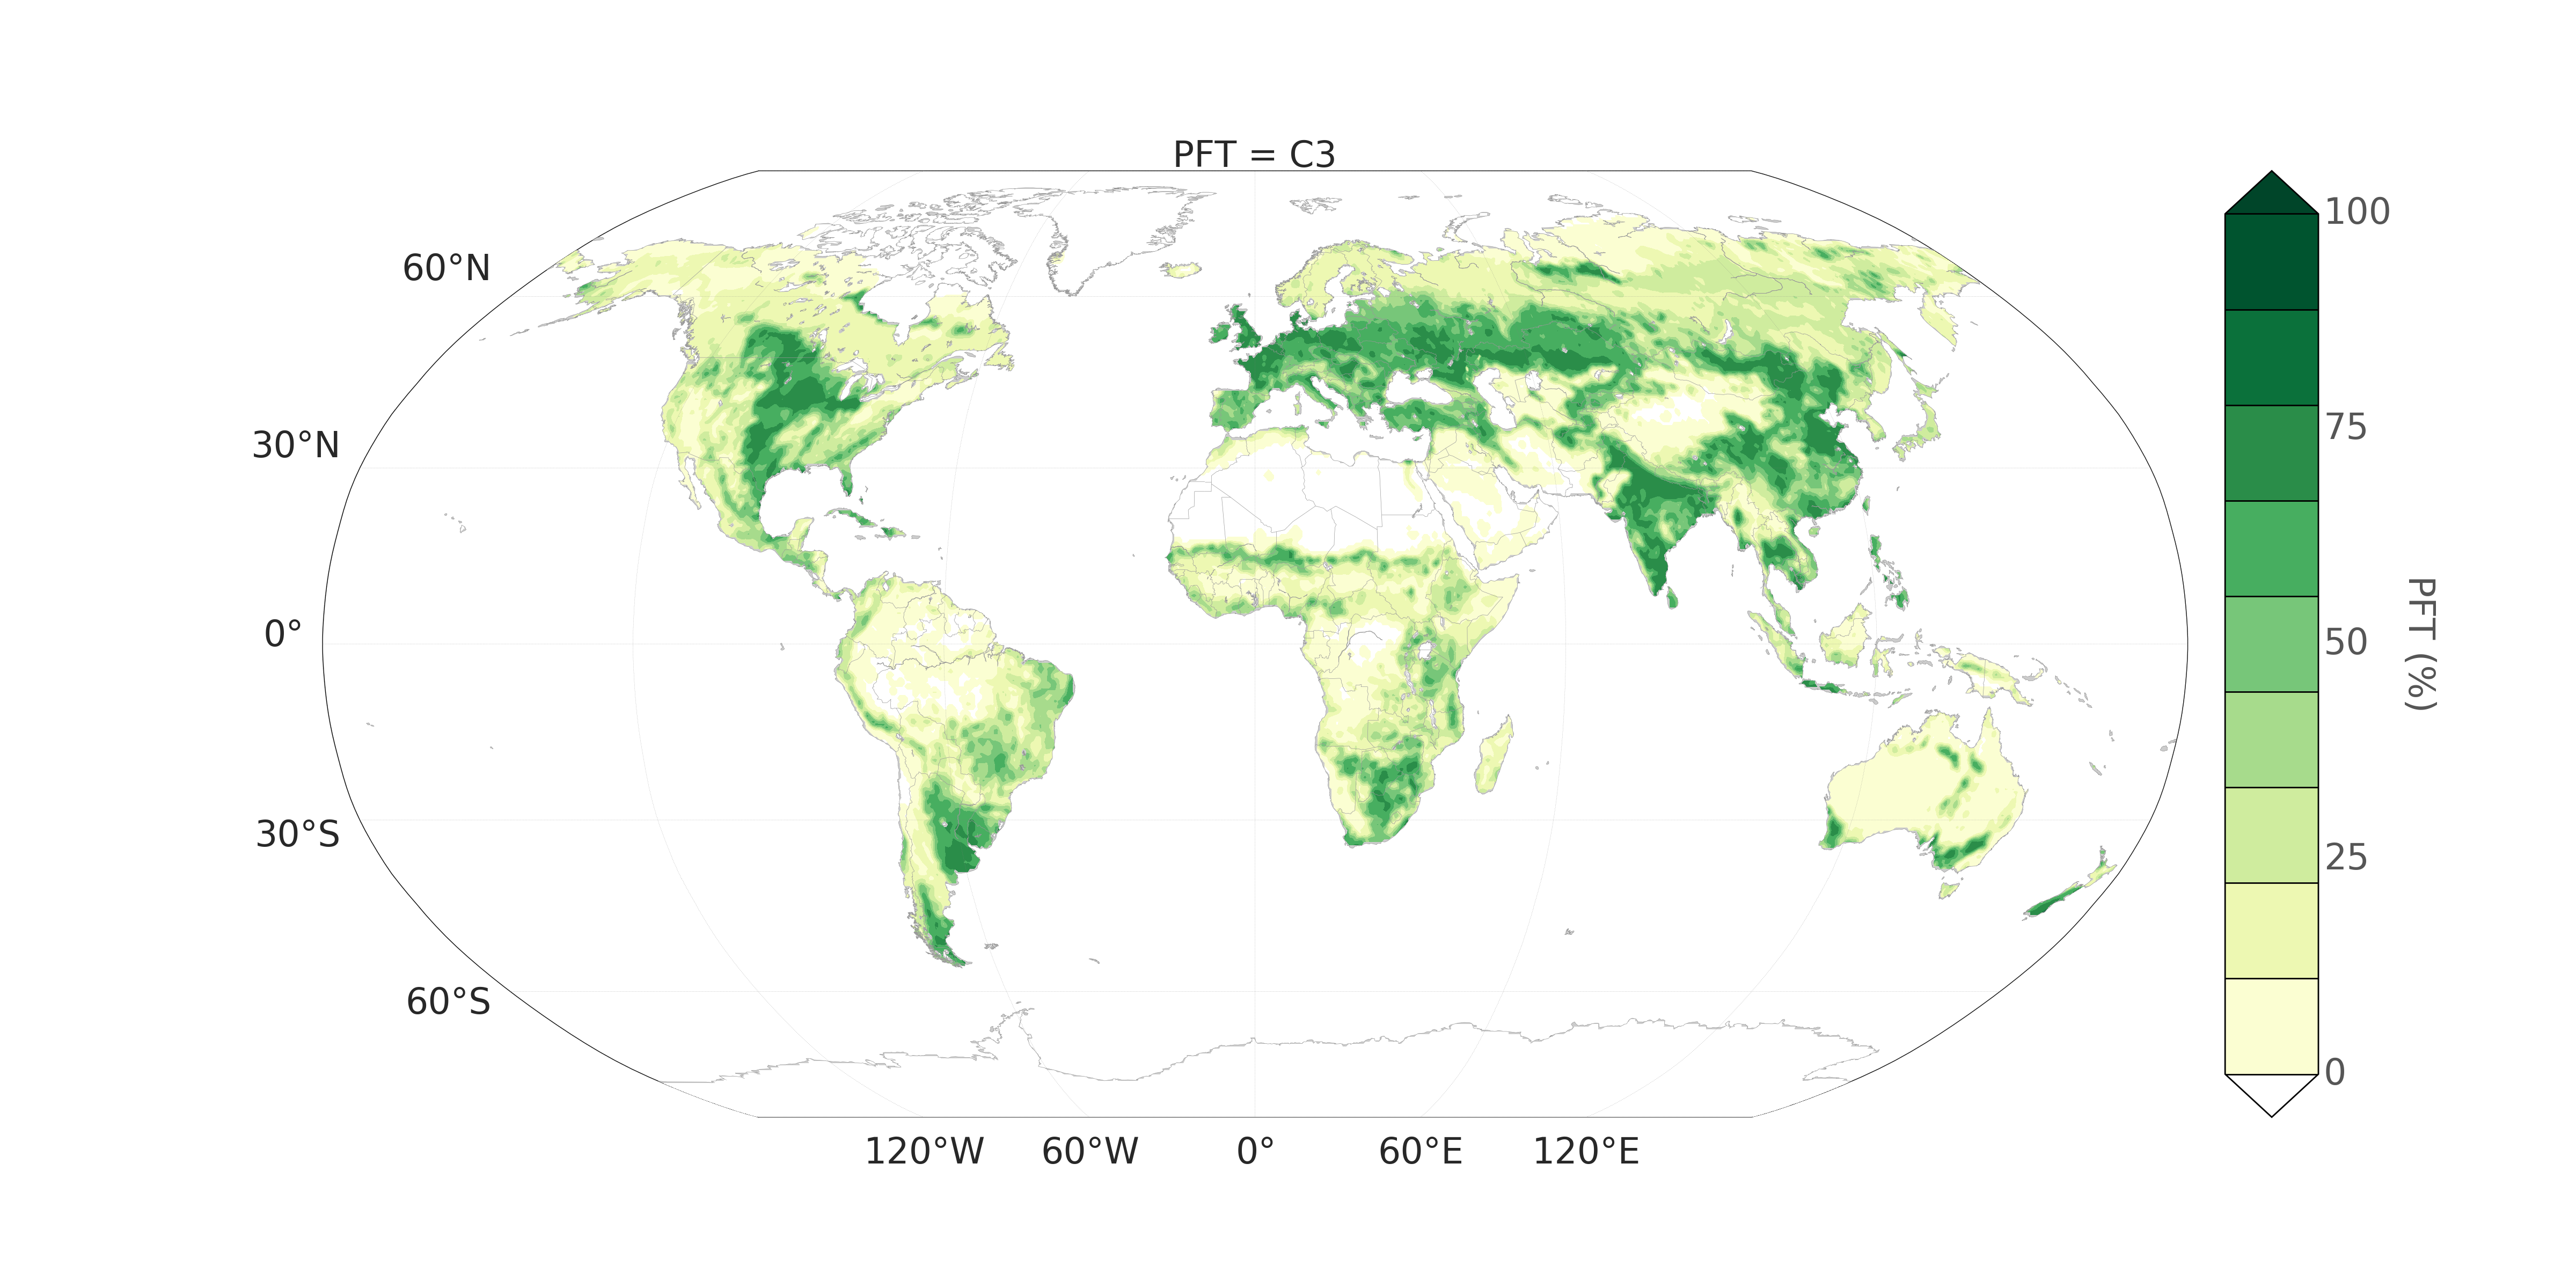
\includegraphics[width=0.5\textwidth]{/home/mn811042/Thesis/chapter6/figures_ofi/PFT_2.png}}
\subfloat[C4]{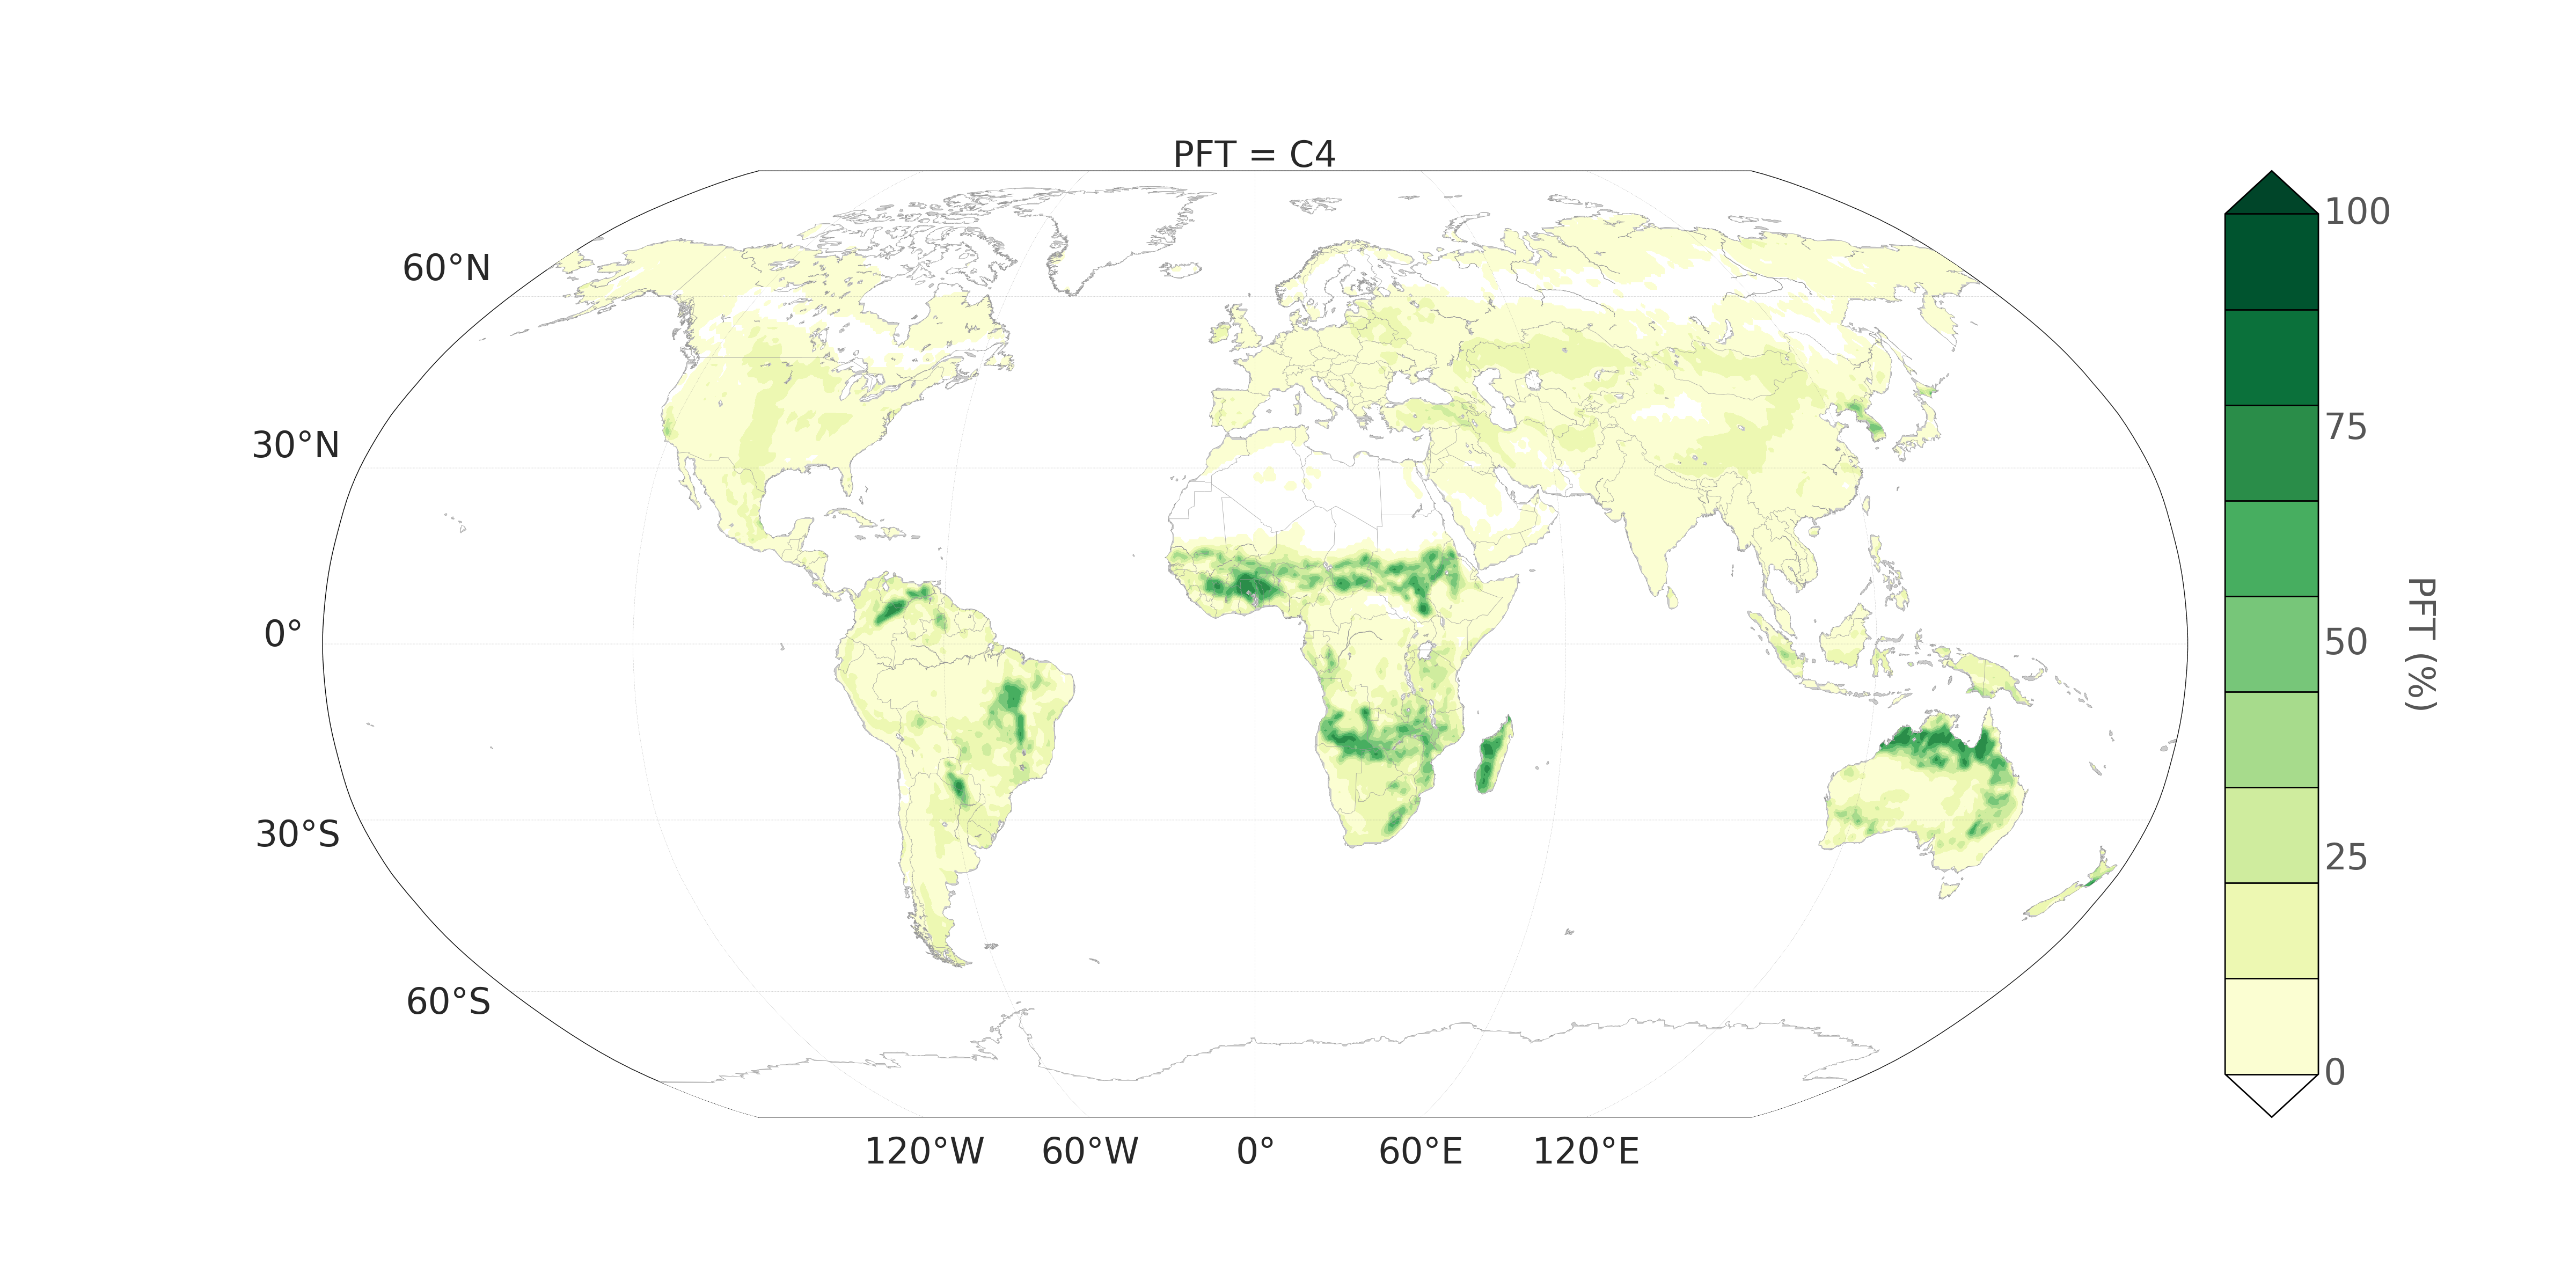
\includegraphics[width=0.5\textwidth]{/home/mn811042/Thesis/chapter6/figures_ofi/PFT_3.png}}
\end{tabular}
\subfloat[SH]{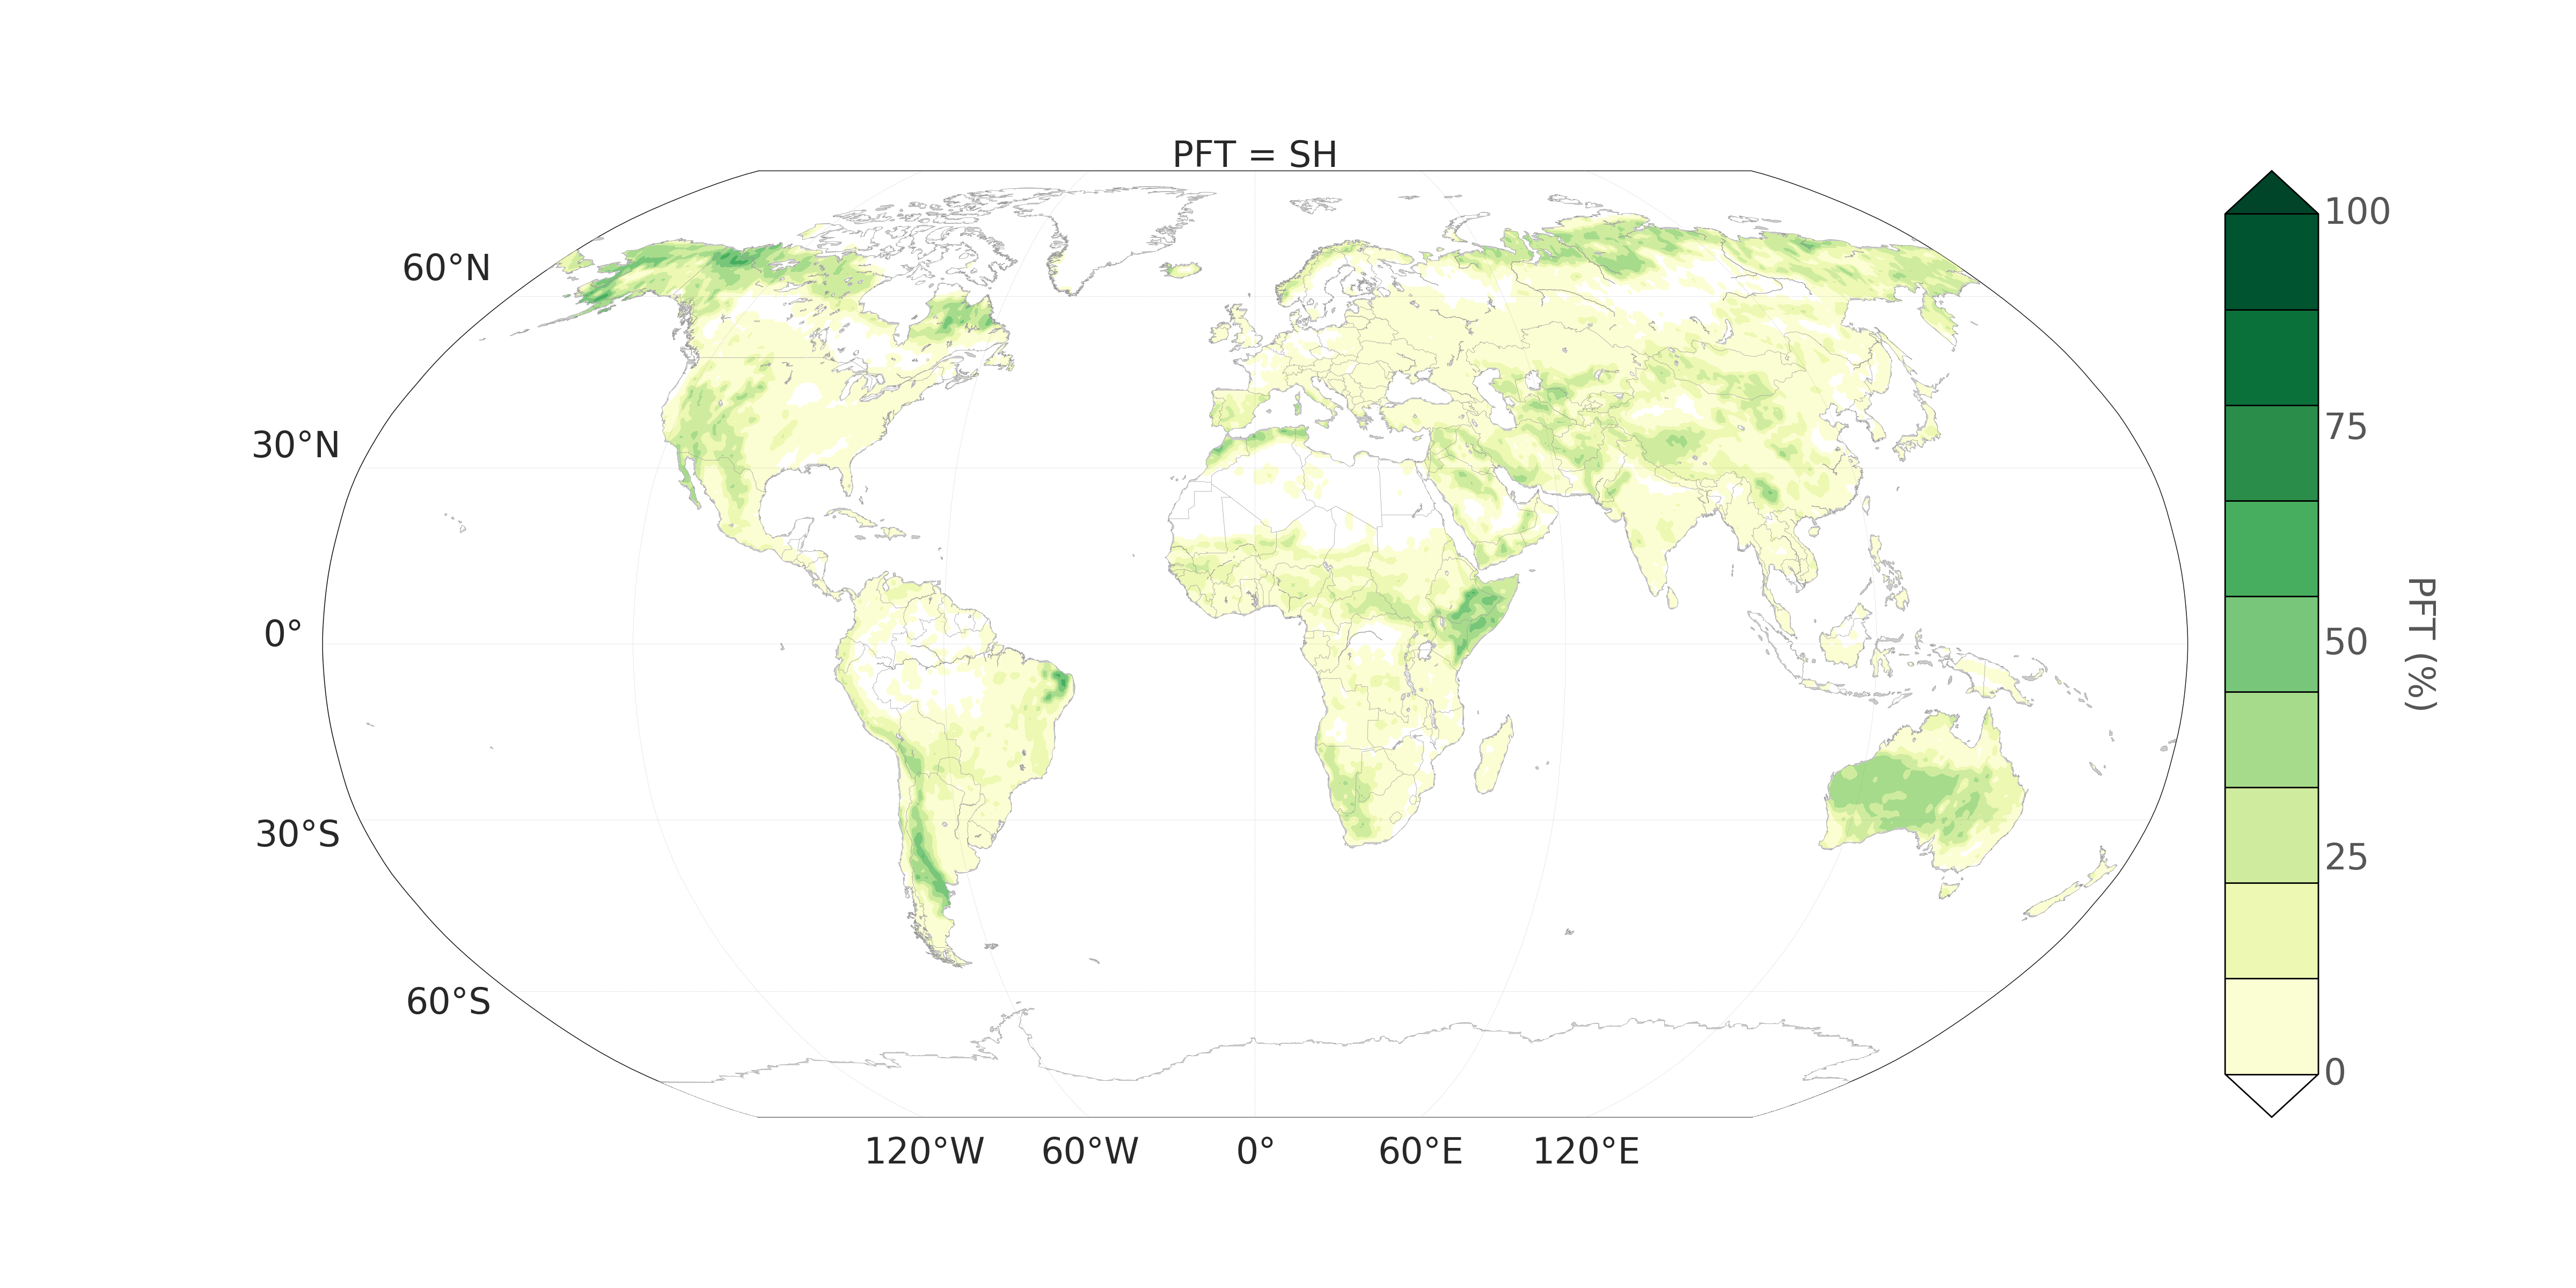
\includegraphics[width=0.5\textwidth]{/home/mn811042/Thesis/chapter6/figures_ofi/PFT_4.png}}
\caption{Distribution of PFTs acording to frac file with global JULES.} 
\label{f:pgap}
\end{figure}

\begin{figure}[ht!]
\centering
\subfloat[Gridbox]{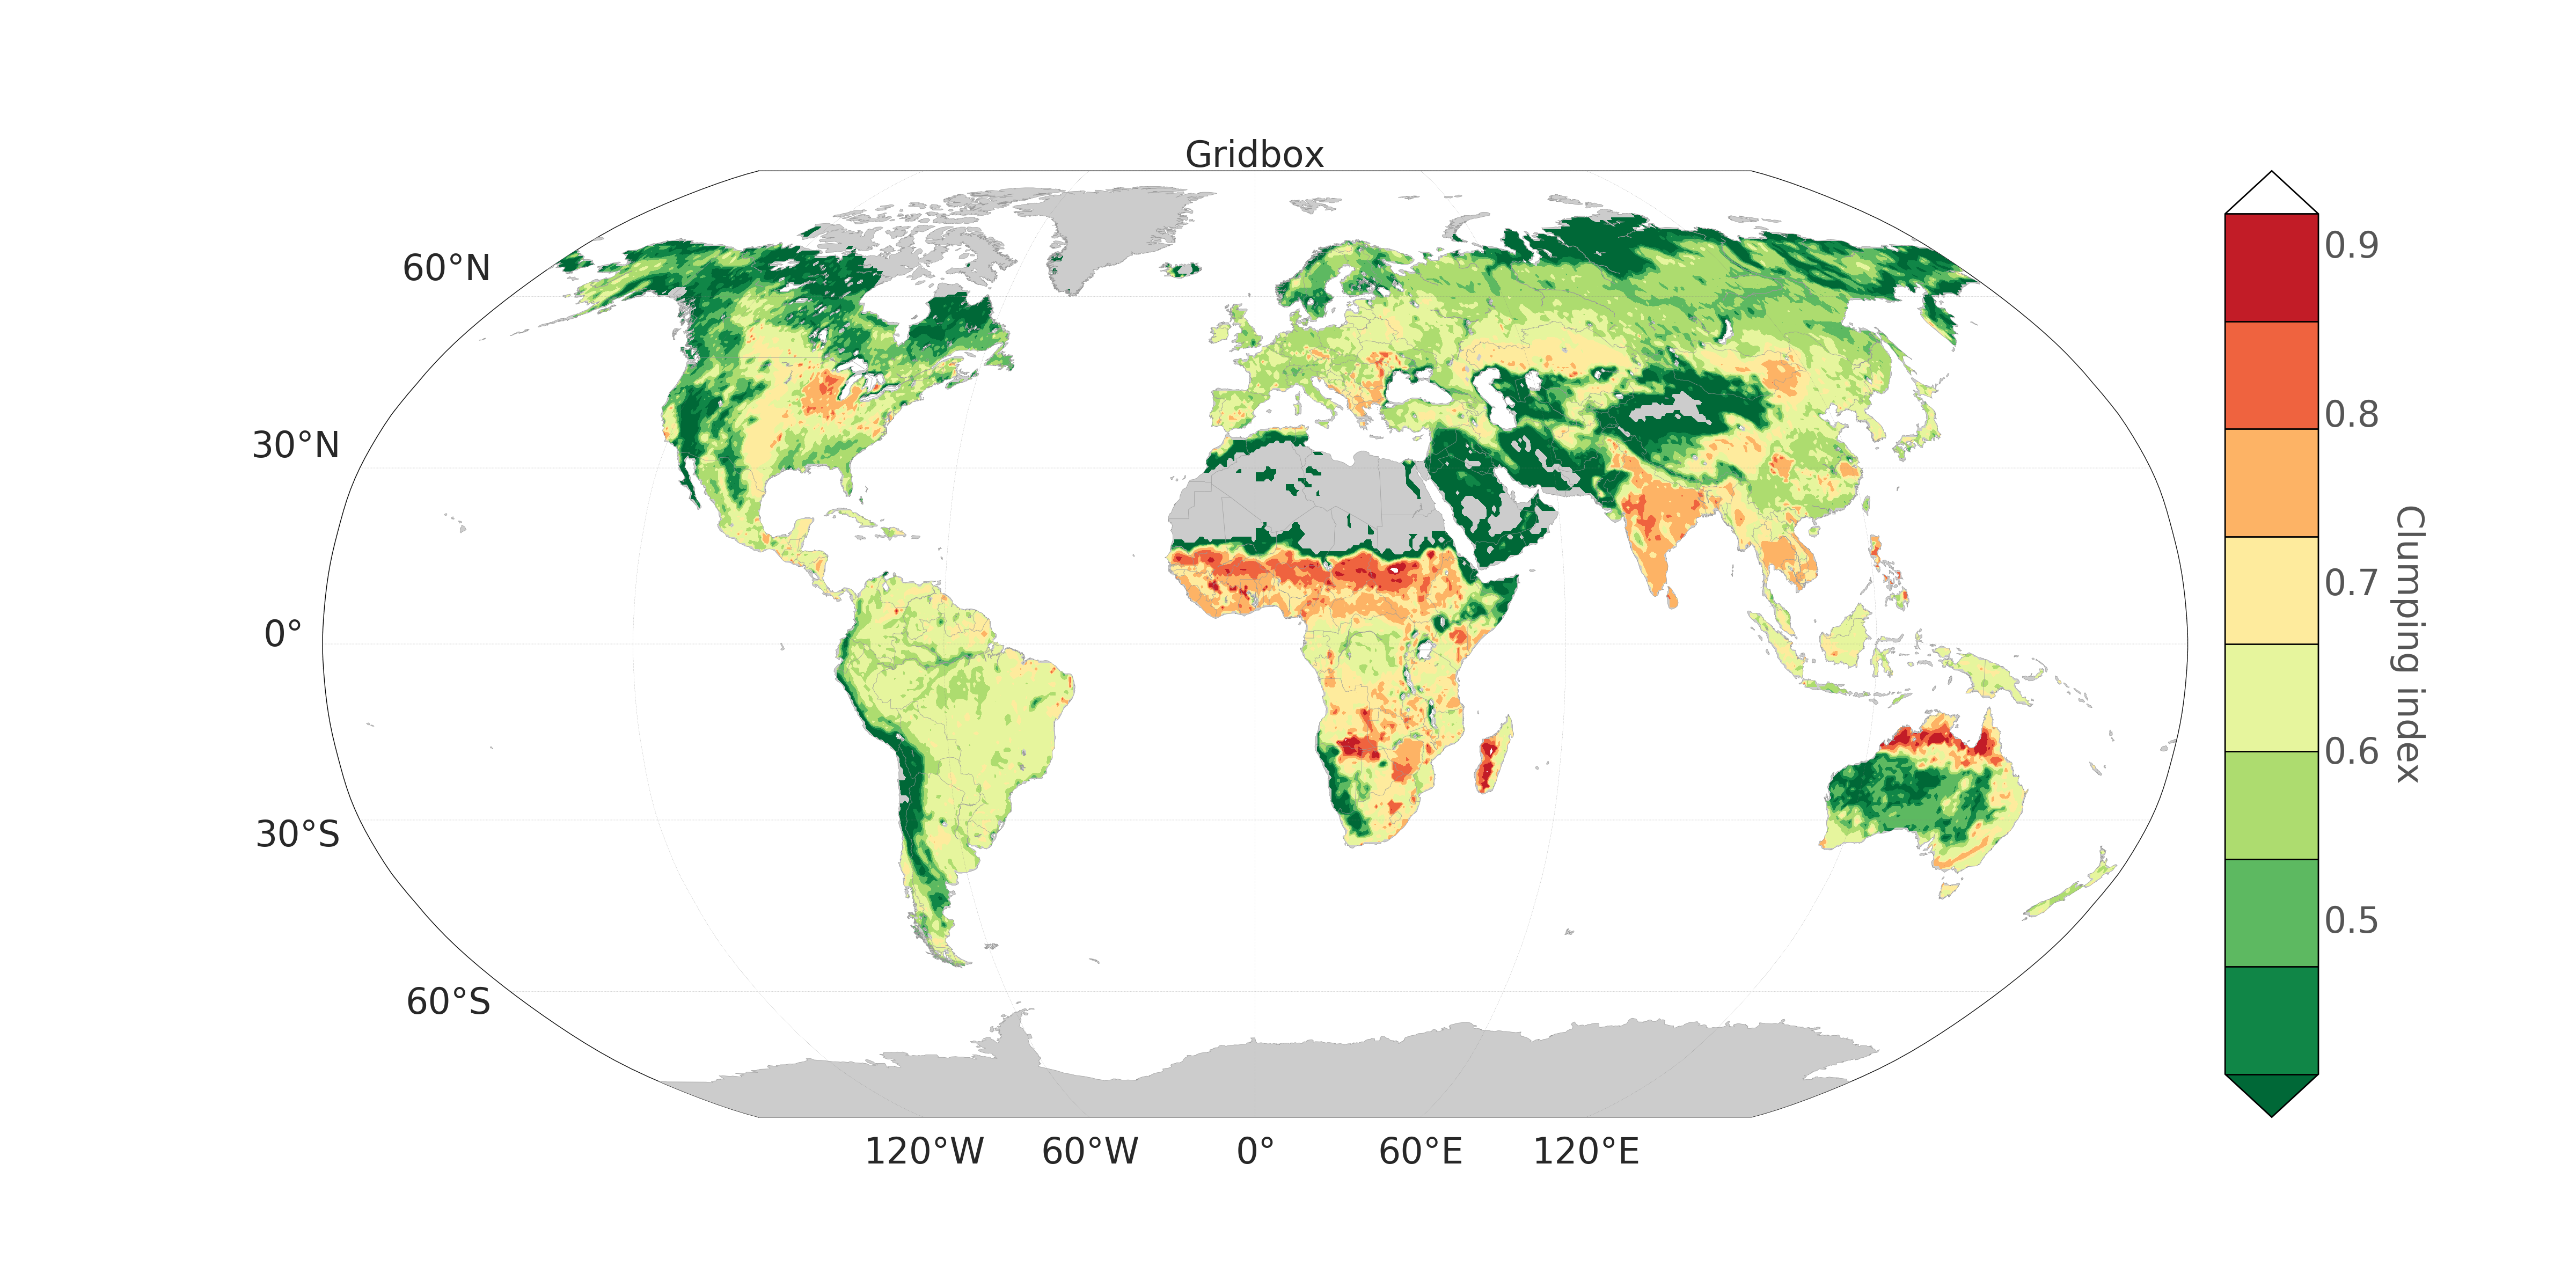
\includegraphics[width=1.0\textwidth]{/home/mn811042/Thesis/chapter6/figures_ofi/clump_PFT_5.png}}
\begin{tabular}{ll}
\subfloat[BL]{\includegraphics[width=0.5\textwidth]{/home/mn811042/Thesis/chapter6/figures_ofi/clump_PFT_0.png}}
\subfloat[NL]{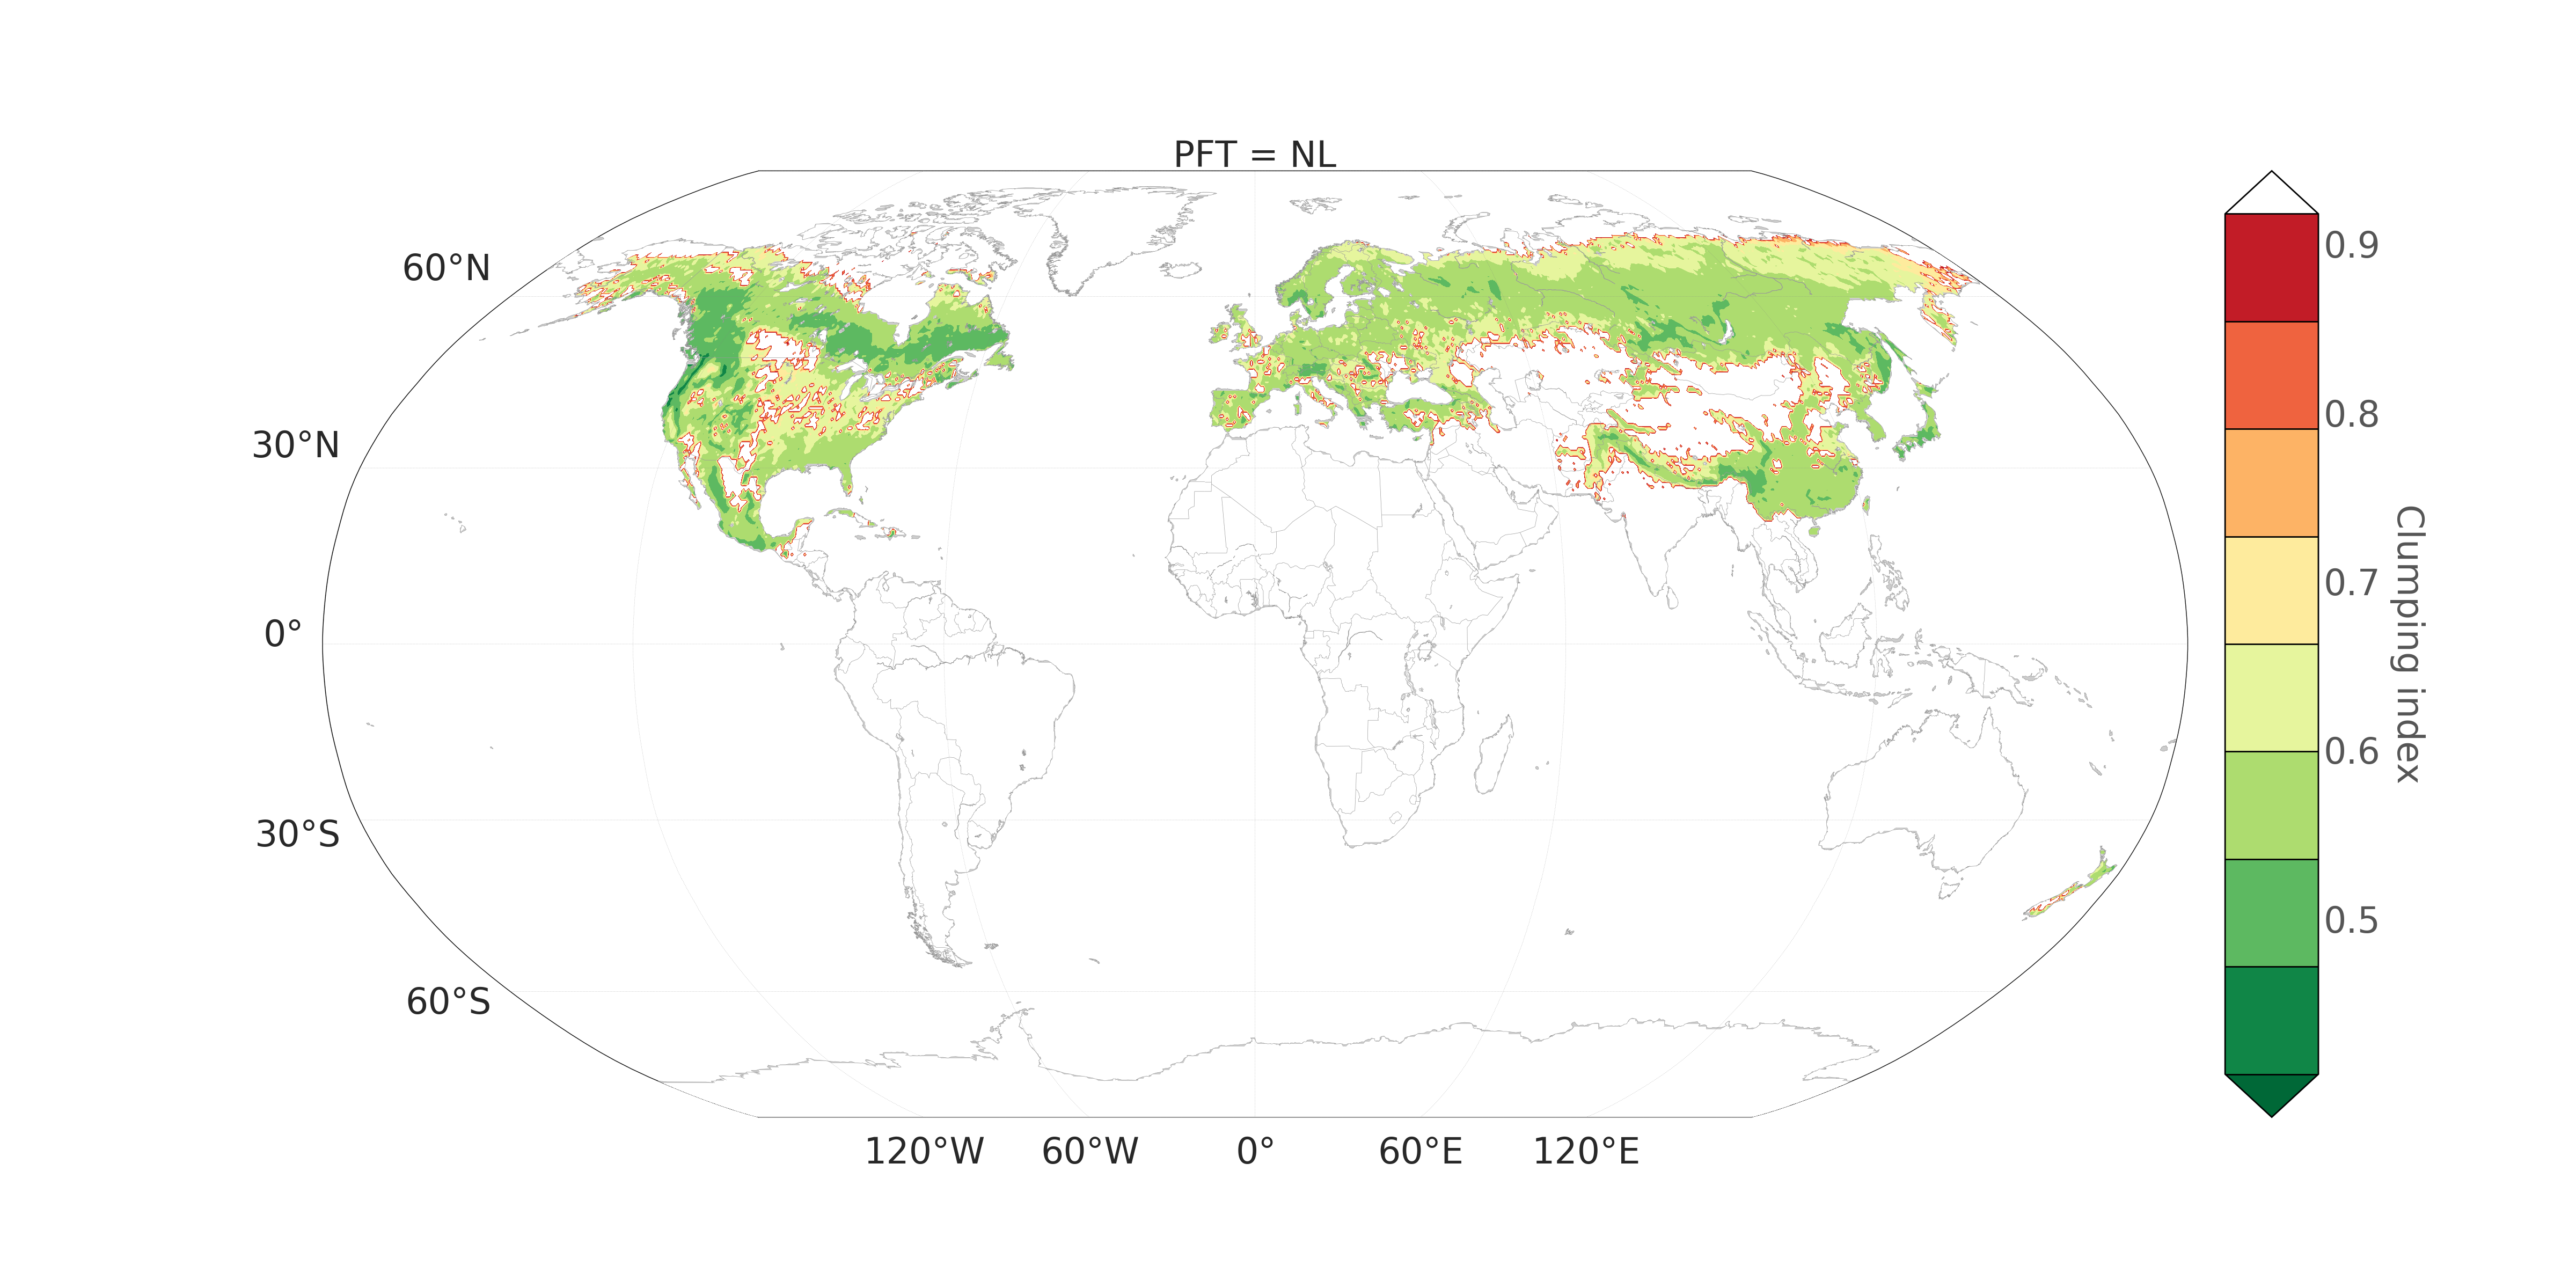
\includegraphics[width=0.5\textwidth]{/home/mn811042/Thesis/chapter6/figures_ofi/clump_PFT_1.png}}
\end{tabular}
\begin{tabular}{ll}
\subfloat[C3]{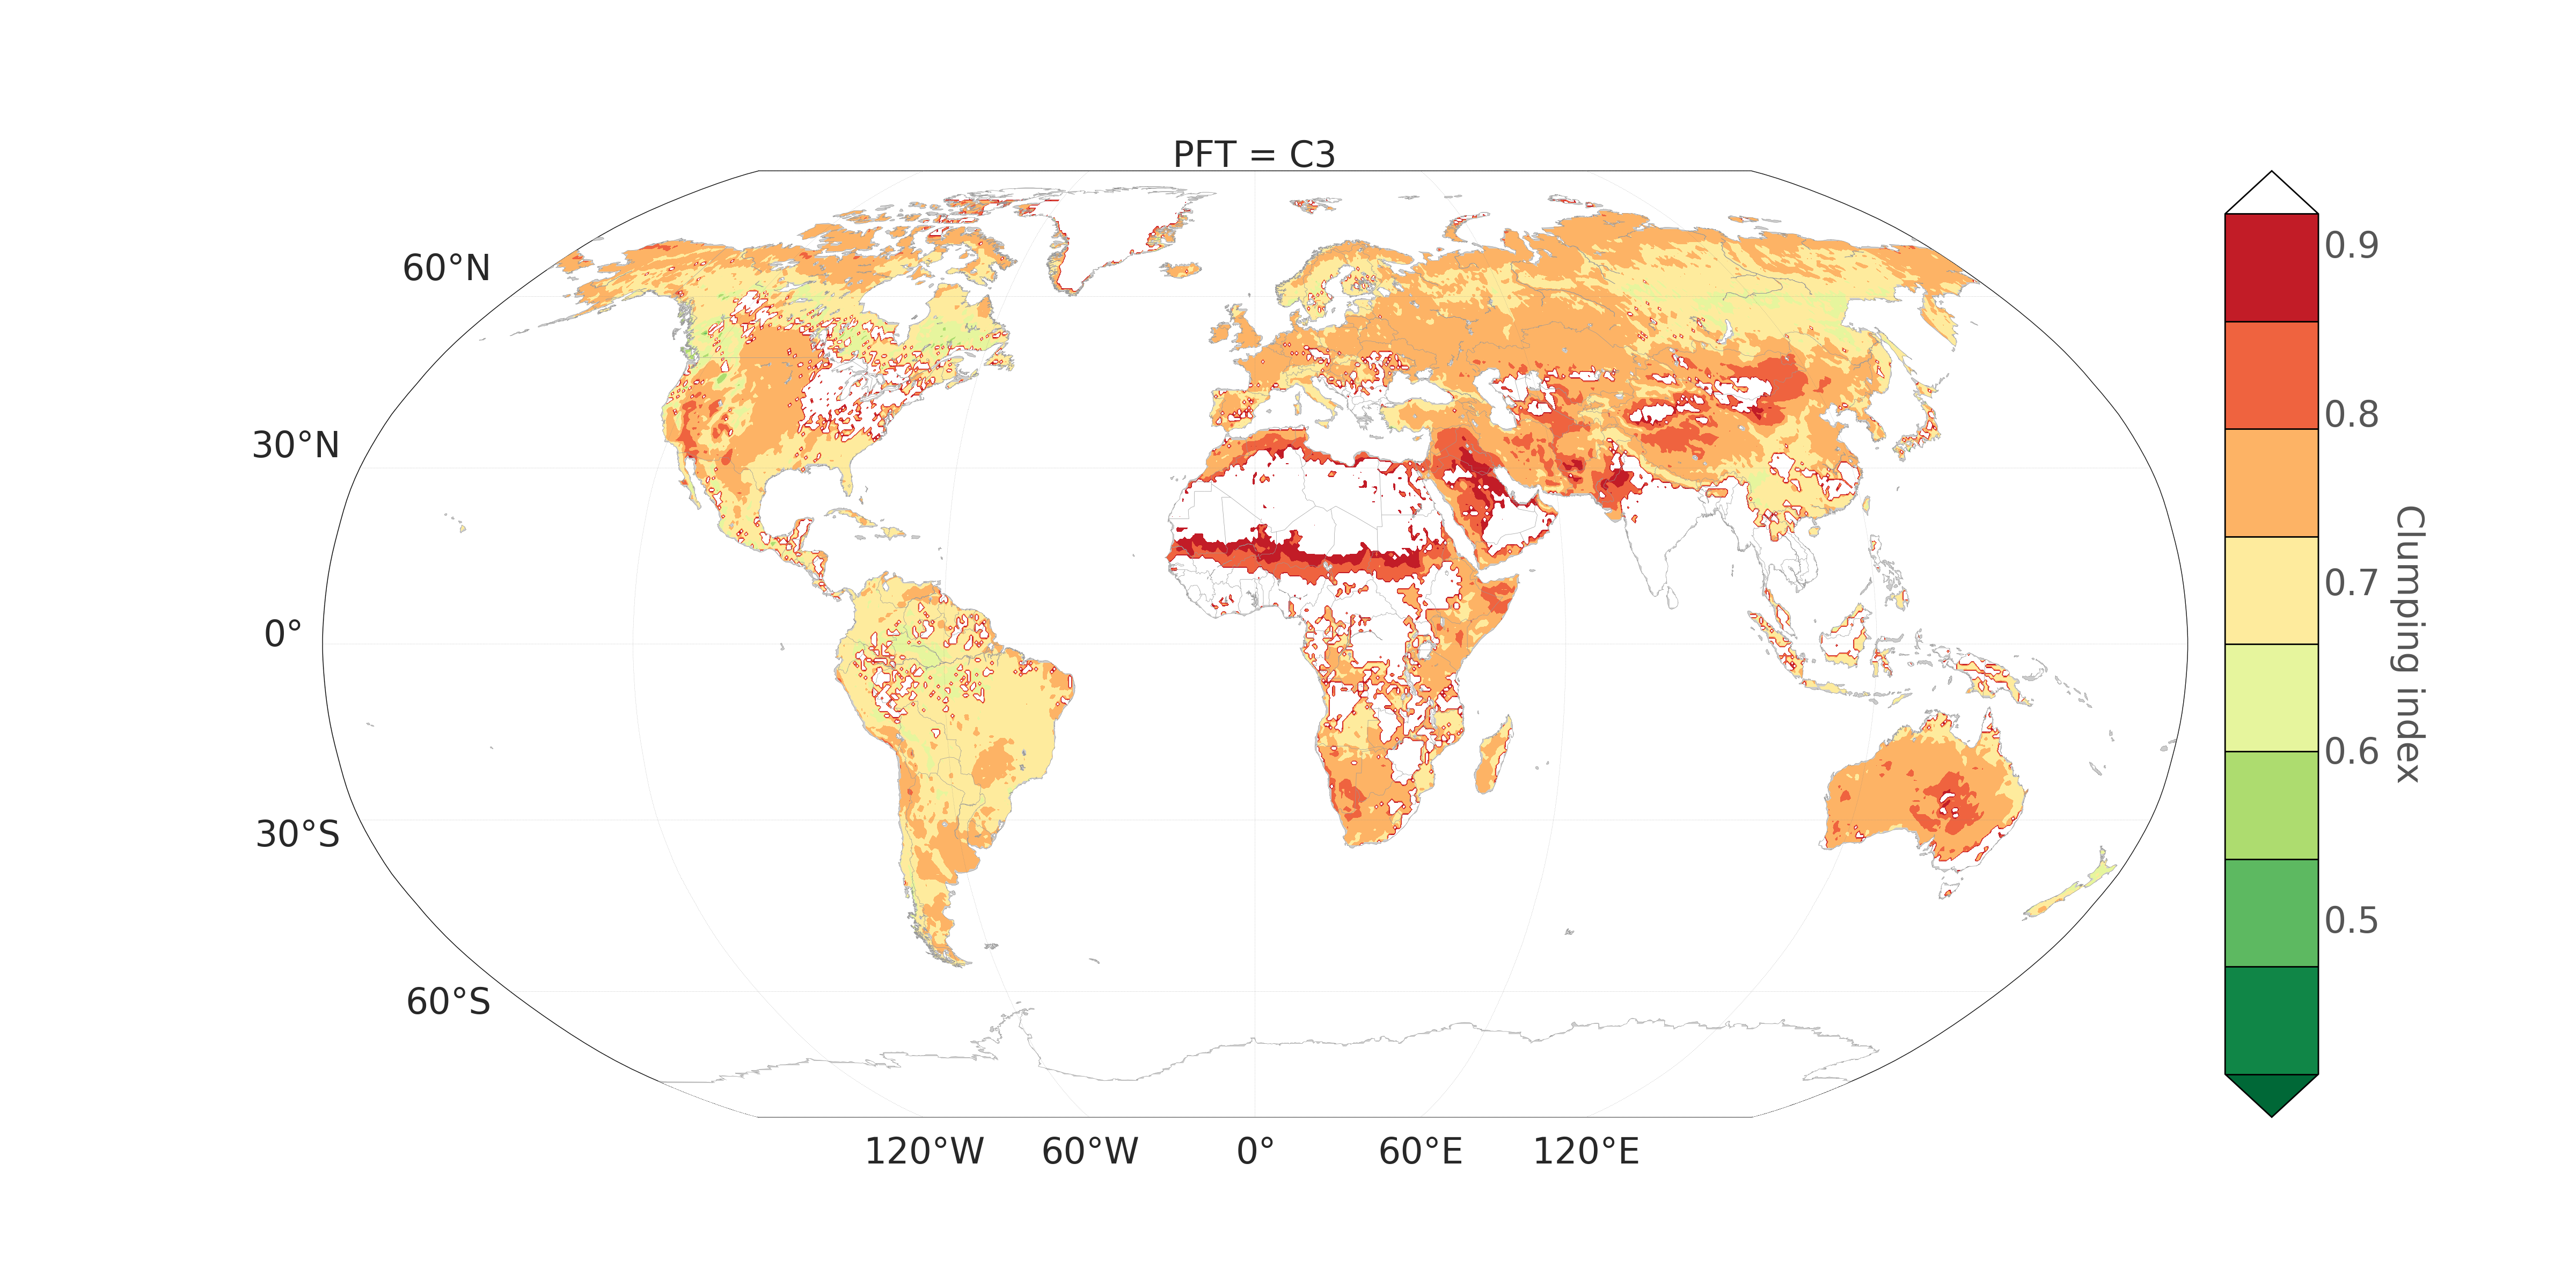
\includegraphics[width=0.5\textwidth]{/home/mn811042/Thesis/chapter6/figures_ofi/clump_PFT_2.png}}
\subfloat[C4]{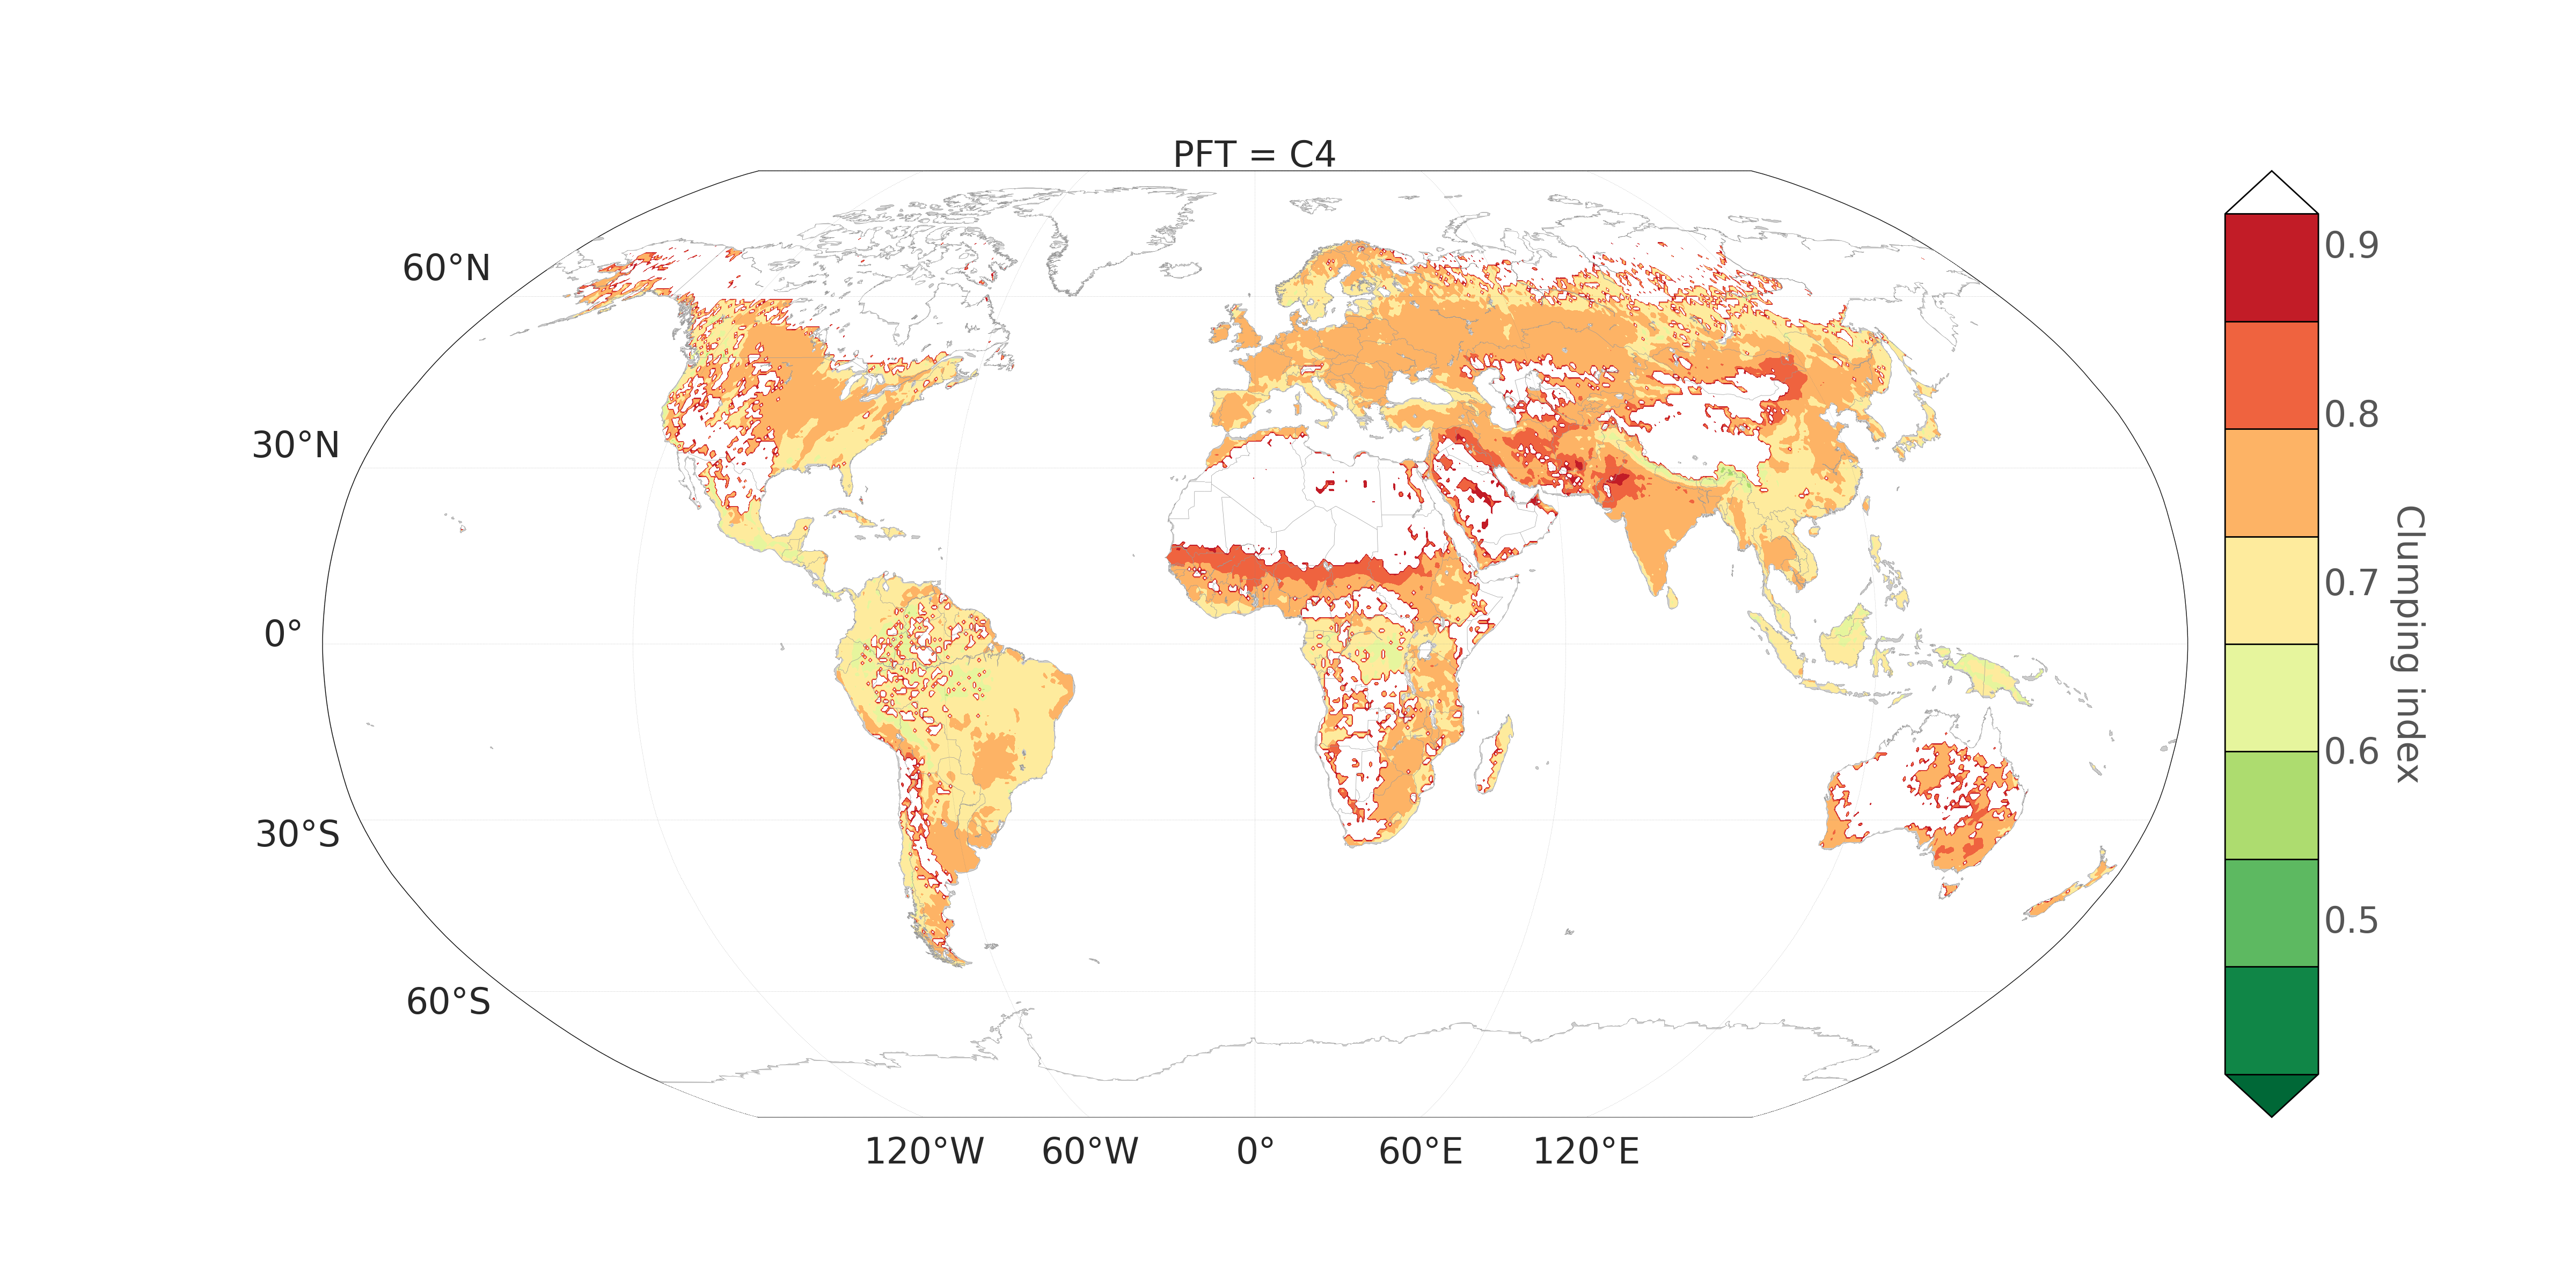
\includegraphics[width=0.5\textwidth]{/home/mn811042/Thesis/chapter6/figures_ofi/clump_PFT_3.png}}
\end{tabular}
\subfloat[SH]{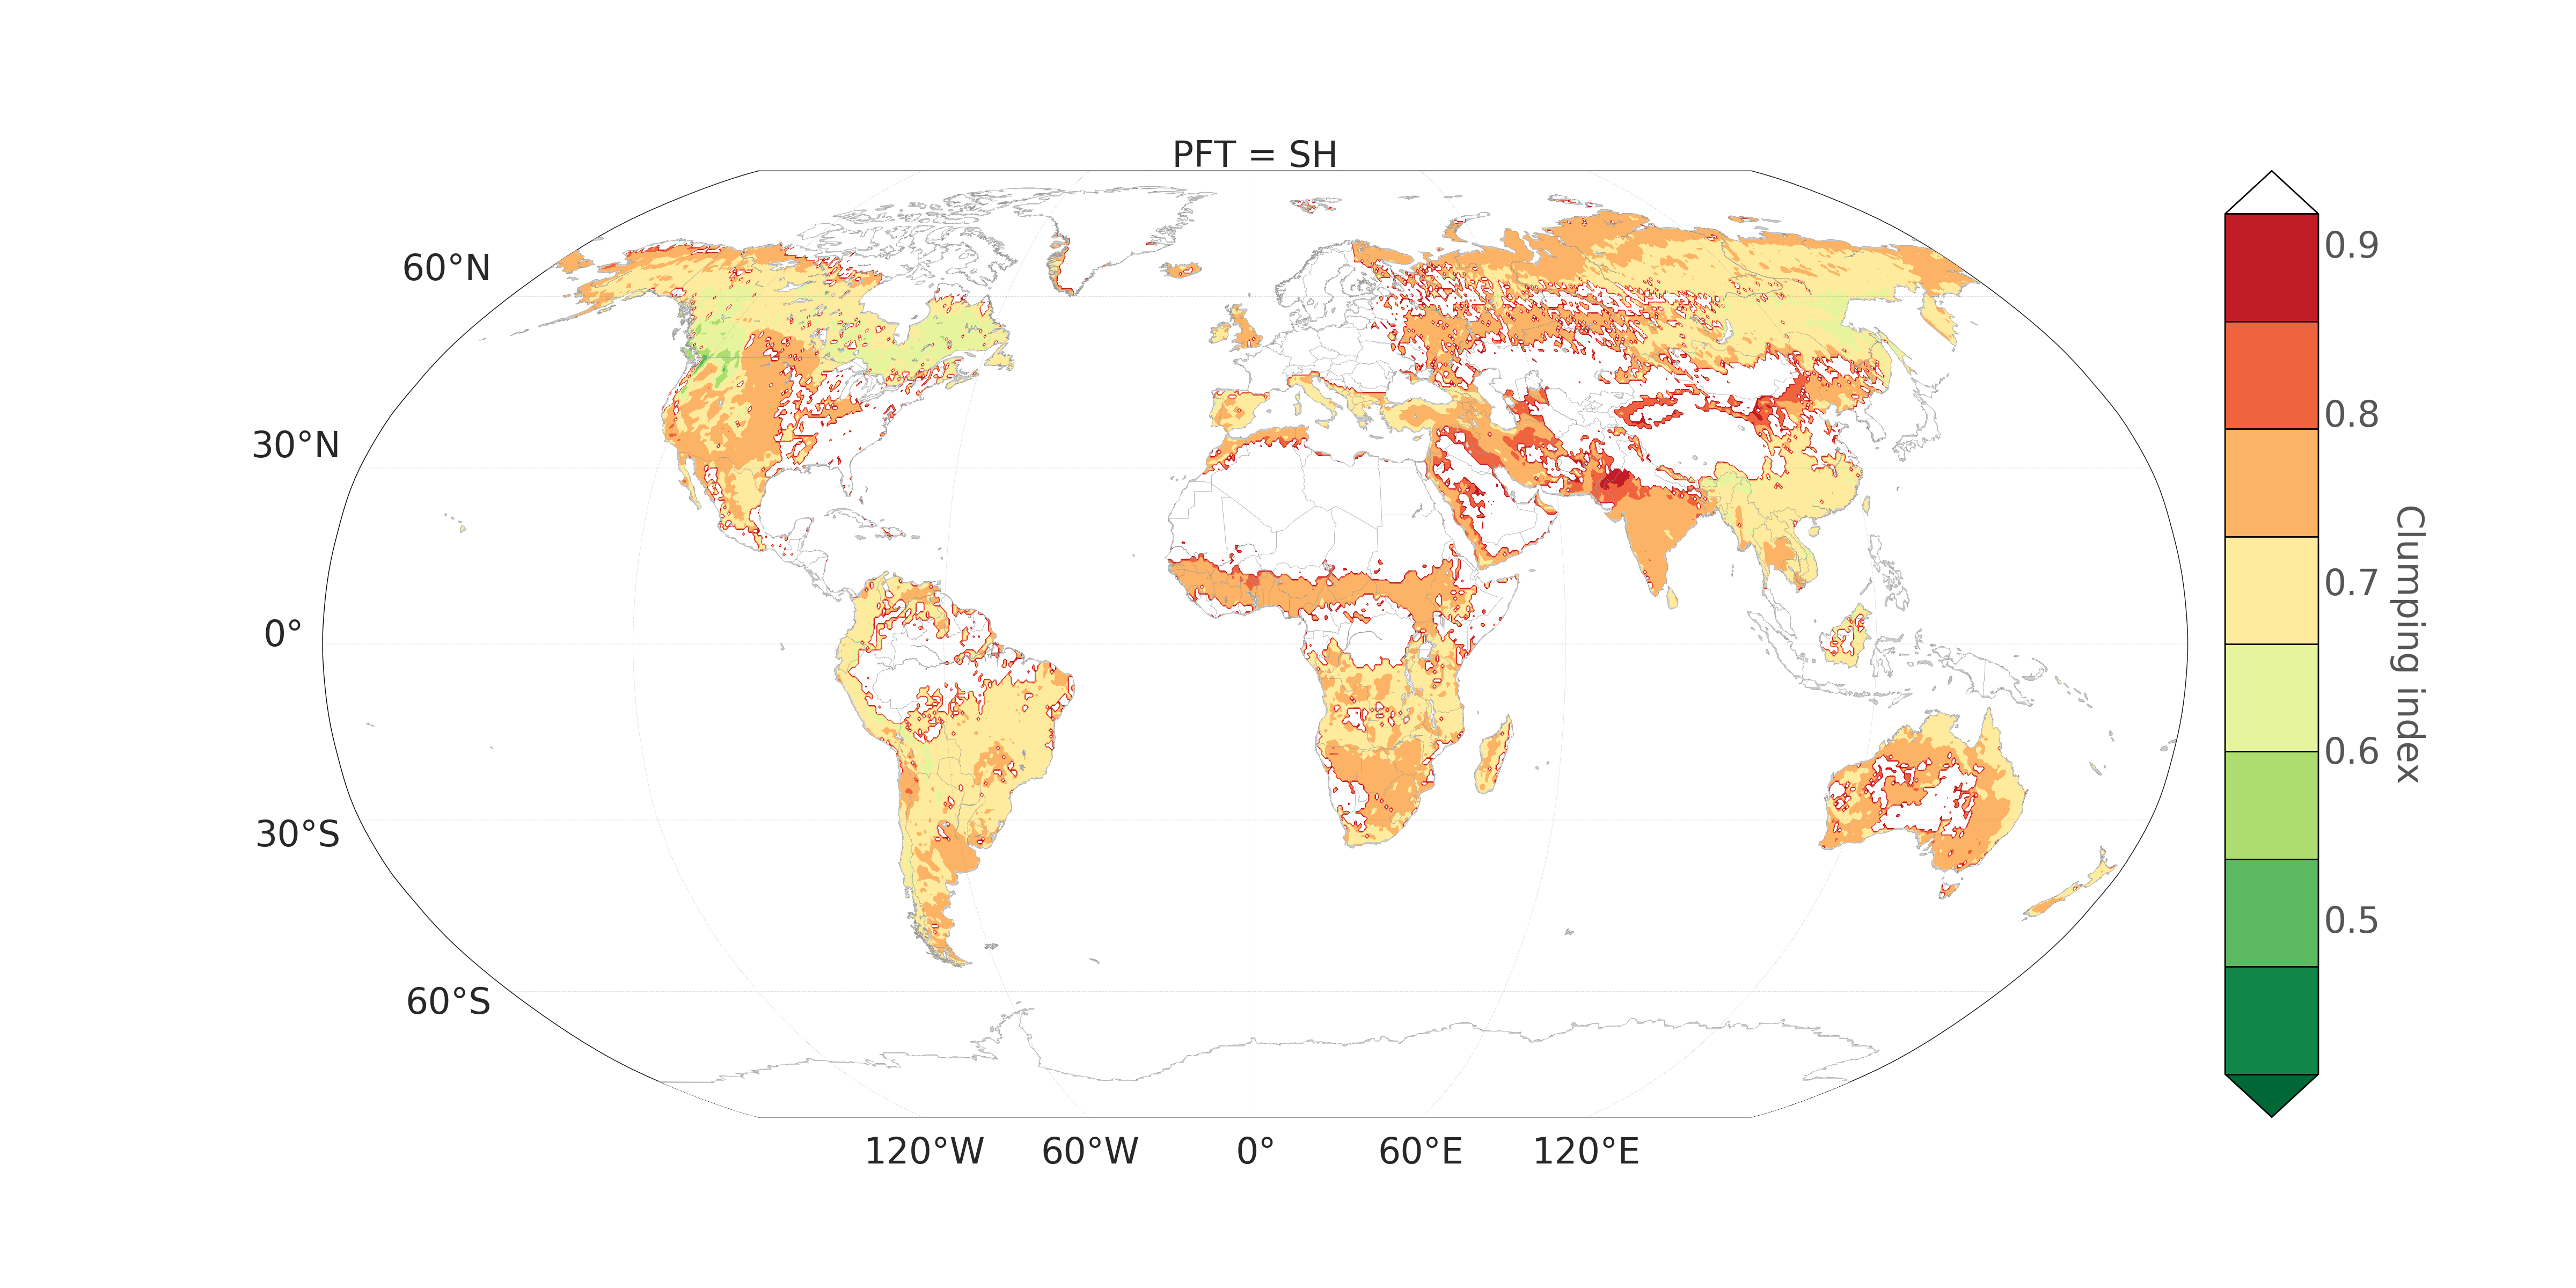
\includegraphics[width=0.5\textwidth]{/home/mn811042/Thesis/chapter6/figures_ofi/clump_PFT_4.png}}
\caption{Distribution of clumping index through PFTs acording to GLC2000 file with global JULES.} 
\label{f:pgap}
\end{figure}

\begin{threeparttable}[ht!]
\centering
\caption{GLC-2000 land cover type to JULES Plant Functional type for clumping index map.}
%\begin{tabular*}{\textwidth}{ l@{\extracolsep{\fill}}*{4}{c}}
\begin{tabular}{l{0.25\textwidth} l{0.75\textwidth}}
%\begin{tabular}{\textwidth}{|p{\textwidth/4}|p{\textwidth/4}|p{\textwidth/4}|p{\textwidth/4}|}
%\begin{tabular*}
     \hline
     \hline
\textbf{GLC-2000 land cover}   & \textbf{JULES PFT}\\
\noalign{\smallskip}\hline
Tree Cover, broadleaved, evergreen                       & Broadleaf\\ 
Tree Cover, broadleaved, deciduous, closed               & Broadleaf\\
Tree Cover, broadleaved, deciduous, open                 & Broadleaf\\
Tree Cover, needle-leaved, evergreen                     & Needle-leaf\\
Tree Cover, needle-leaved, deciduous                     & Needle-leaf\\
Tree Cover, mixed leaf type                              & Broadleaf\\
Tree Cover, regularly flooded, fresh  water              & Broadleaf\\
Tree Cover, regularly flooded, saline water              & Broadleaf\\
Mosaic: Tree cover / Other natural vegetation            & Broadleaf\\
Tree Cover, burnt                                        & Broadleaf\\
Shrub Cover, closed-open, evergreen                      & Shrub\\
Shrub Cover, closed-open, deciduous                      & Shrub\\
Herbaceous Cover, closed-open                            & C3\\
Sparse Herbaceous or sparse Shrub Cover                  & C3\\
Regularly flooded Shrub and/or Herbaceous Cover          & C3\\
Cultivated and managed areas                             & C4\\
Mosaic: Cropland / Tree Cover / Other natural vegetation & C4\\
Mosaic: Cropland / Shrub or Grass Cover                  & C4\\
Bare Areas                                               & \textit{NA}\\
Water Bodies                                             & \textit{NA}\\
Snow and Ice                                             & \textit{NA}\\
Artificial surfaces and associated areas                 & \textit{NA}\\
No data                                                  & \textit{NA}\\
\hline
\hline%\noalign{\bigskip}
%\end{tabular*}
\end{tabular}
\begin{tablenotes}
      \small
      \item \textit{NA}: Not applicable. 
\end{tablenotes}
\label{tab:RAMI4PILPS}
\end{threeparttable}
\bigskip


\begin{figure}[ht!]
\centering
\begin{tabular}{ll}
\subfloat[Opt 4 - MTE]{\includegraphics[width=0.5\textwidth]{/home/mn811042/Thesis/chapter6/figures_ofi/adjust_4_mte_filtered_2.png}}
\subfloat[Opt 4 clump - MTE]{\includegraphics[width=0.5\textwidth]{/home/mn811042/Thesis/chapter6/figures_ofi/adjust_4_clump_mte_filtered_2.png}}
\end{tabular}
\begin{tabular}{ll}
\subfloat[Opt 4 - BL]{\includegraphics[width=0.5\textwidth]{/home/mn811042/Thesis/chapter6/figures_ofi/adjust_opt4_pft_0_filtered_3.png}}
\subfloat[Opt 4 clump - BL]{\includegraphics[width=0.5\textwidth]{/home/mn811042/Thesis/chapter6/figures_ofi/adjust_opt4_clump_pft_0_filtered_3.png}}
\end{tabular}
\begin{tabular}{ll}
\subfloat[Opt 4 - NL]{\includegraphics[width=0.5\textwidth]{/home/mn811042/Thesis/chapter6/figures_ofi/adjust_opt4_pft_1_filtered_3.png}}
\subfloat[Opt 4 clump - NL]{\includegraphics[width=0.5\textwidth]{/home/mn811042/Thesis/chapter6/figures_ofi/adjust_opt4_clump_pft_1_filtered_3.png}}
\end{tabular}
\caption{Comparison of JULES GPP through option 5 and the version with structure versus MTE applied only where the fraction of each gridbox is higher than 50\%  for the year of 2008.} 
\label{f:pgap}
\end{figure}


\begin{figure}[ht!]
\centering
\begin{tabular}{ll}
\subfloat[Opt 4 - C3]{\includegraphics[width=0.5\textwidth]{/home/mn811042/Thesis/chapter6/figures_ofi/adjust_opt4_pft_2_filtered_3.png}}
\subfloat[Opt 4 clump - C3]{\includegraphics[width=0.5\textwidth]{/home/mn811042/Thesis/chapter6/figures_ofi/adjust_opt4_clump_pft_2_filtered_3.png}}
\end{tabular}
\begin{tabular}{ll}
\subfloat[Opt 4 - C4]{\includegraphics[width=0.5\textwidth]{/home/mn811042/Thesis/chapter6/figures_ofi/adjust_opt4_pft_3_filtered_3.png}}
\subfloat[Opt 4 clump - C4]{\includegraphics[width=0.5\textwidth]{/home/mn811042/Thesis/chapter6/figures_ofi/adjust_opt4_clump_pft_3_filtered_3.png}}
\end{tabular}
\begin{tabular}{ll}
\subfloat[Opt 4 - SH]{\includegraphics[width=0.5\textwidth]{/home/mn811042/Thesis/chapter6/figures_ofi/adjust_opt4_pft_4_filtered_3.png}}
\subfloat[Opt 4 clump - SH]{\includegraphics[width=0.5\textwidth]{/home/mn811042/Thesis/chapter6/figures_ofi/adjust_opt4_clump_pft_4_filtered_3.png}}
\end{tabular}
\caption{Comparison of JULES GPP through option 5 and the version with structure versus MTE applied only where the fraction of each gridbox is higher than 50\%  for the year of 2008.} 
\label{f:pgap}
\end{figure}

\begin{figure}[ht!]
\centering
\begin{tabular}{ll}
\subfloat[Opt 5 - MTE]{\includegraphics[width=0.5\textwidth]{/home/mn811042/Thesis/chapter6/figures_ofi/adjust_5_mte_filtered_2.png}}
\subfloat[Opt 5 clump - MTE]{\includegraphics[width=0.5\textwidth]{/home/mn811042/Thesis/chapter6/figures_ofi/adjust_5_clump_mte_filtered_2.png}}
\end{tabular}
\begin{tabular}{ll}
\subfloat[Opt 5 - BL]{\includegraphics[width=0.5\textwidth]{/home/mn811042/Thesis/chapter6/figures_ofi/adjust_opt5_pft_0_filtered_3.png}}
\subfloat[Opt 5 clump - BL]{\includegraphics[width=0.5\textwidth]{/home/mn811042/Thesis/chapter6/figures_ofi/adjust_opt5_clump_pft_0_filtered_3.png}}
\end{tabular}
\begin{tabular}{ll}
\subfloat[Opt 5 - NL]{\includegraphics[width=0.5\textwidth]{/home/mn811042/Thesis/chapter6/figures_ofi/adjust_opt5_pft_1_filtered_3.png}}
\subfloat[Opt 5 clump - NL]{\includegraphics[width=0.5\textwidth]{/home/mn811042/Thesis/chapter6/figures_ofi/adjust_opt5_clump_pft_1_filtered_3.png}}
\end{tabular}
\caption{Comparison of JULES GPP through option 5 and the version with structure versus MTE applied only where the fraction of each gridbox is higher than 50\% for the year of 2008.} 
\label{f:pgap}
\end{figure}


\begin{figure}[ht!]
\centering
\begin{tabular}{ll}
\subfloat[Opt 5 - C3]{\includegraphics[width=0.5\textwidth]{/home/mn811042/Thesis/chapter6/figures_ofi/adjust_opt5_pft_2_filtered_3.png}}
\subfloat[Opt 5 clump - C3]{\includegraphics[width=0.5\textwidth]{/home/mn811042/Thesis/chapter6/figures_ofi/adjust_opt5_clump_pft_2_filtered_3.png}}
\end{tabular}
\begin{tabular}{ll}
\subfloat[Opt 5 - C4]{\includegraphics[width=0.5\textwidth]{/home/mn811042/Thesis/chapter6/figures_ofi/adjust_opt5_pft_3_filtered_3.png}}
\subfloat[Opt 5 clump - C4]{\includegraphics[width=0.5\textwidth]{/home/mn811042/Thesis/chapter6/figures_ofi/adjust_opt5_clump_pft_3_filtered_3.png}}
\end{tabular}
\begin{tabular}{ll}
\subfloat[Opt 5 - SH]{\includegraphics[width=0.5\textwidth]{/home/mn811042/Thesis/chapter6/figures_ofi/adjust_opt5_pft_4_filtered_3.png}}
\subfloat[Opt 5 clump - SH]{\includegraphics[width=0.5\textwidth]{/home/mn811042/Thesis/chapter6/figures_ofi/adjust_opt5_clump_pft_4_filtered_3.png}}
\end{tabular}
\caption{Comparison of JULES GPP through option 5 and the version with structure versus MTE applied only where the fraction of each gridbox is higher than 50\%  for the year of 2008.} 
\label{f:pgap}
\end{figure}


\begin{figure}[ht!]
\centering\hspace*{-1.9in}
\begin{tabular}{ll}
\subfloat[Diff Opt 4 clump - 4]{\includegraphics[width=0.7\textwidth]{/home/mn811042/Thesis/chapter6/figures_ofi/jules_anom_opt4_clump_MR_year.png}}
\subfloat[Diff Opt 5 clump - 5]{\includegraphics[width=0.7\textwidth]{/home/mn811042/Thesis/chapter6/figures_ofi/jules_anom_opt5_clump_MR_year.png}}
\end{tabular}
\centering\hspace*{-1.9in}
\begin{tabular}{ll}
\subfloat[Opt 4 BL]{\includegraphics[width=0.7\textwidth]{/home/mn811042/Thesis/chapter6/figures_ofi/jules_anom_opt4_pft_0_clump_MR_year.png}}
\subfloat[Opt 5 BL]{\includegraphics[width=0.7\textwidth]{/home/mn811042/Thesis/chapter6/figures_ofi/jules_anom_opt5_pft_0_clump_MR_year.png}}
\end{tabular}
\centering\hspace*{-1.9in}
\begin{tabular}{ll}
\subfloat[Opt 4 NL]{\includegraphics[width=0.7\textwidth]{/home/mn811042/Thesis/chapter6/figures_ofi/jules_anom_opt4_pft_1_clump_MR_year.png}}
\subfloat[Opt 5 NL]{\includegraphics[width=0.7\textwidth]{/home/mn811042/Thesis/chapter6/figures_ofi/jules_anom_opt5_pft_1_clump_MR_year.png}}
\end{tabular}

\caption{Spatial impact of clumping per PFT for two radiative transfer modules in JULES.} 
\label{f:pgap}
\end{figure}


\begin{figure}[ht!]
\centering\hspace*{-1.9in}
\begin{tabular}{ll}
\subfloat[Opt 4 C3]{\includegraphics[width=0.7\textwidth]{/home/mn811042/Thesis/chapter6/figures_ofi/jules_anom_opt4_pft_2_clump_MR_year.png}}
\subfloat[Opt 5 C3]{\includegraphics[width=0.7\textwidth]{/home/mn811042/Thesis/chapter6/figures_ofi/jules_anom_opt5_pft_2_clump_MR_year.png}}
\end{tabular}
\centering\hspace*{-1.9in}
\begin{tabular}{ll}
\subfloat[Opt 4 C4]{\includegraphics[width=0.7\textwidth]{/home/mn811042/Thesis/chapter6/figures_ofi/jules_anom_opt4_pft_3_clump_MR_year.png}}
\subfloat[Opt 5 C4]{\includegraphics[width=0.7\textwidth]{/home/mn811042/Thesis/chapter6/figures_ofi/jules_anom_opt5_pft_3_clump_MR_year.png}}
\end{tabular}
\centering\hspace*{-1.9in}
\begin{tabular}{ll}
\subfloat[Opt 4 SH]{\includegraphics[width=0.7\textwidth]{/home/mn811042/Thesis/chapter6/figures_ofi/jules_anom_opt4_pft_4_clump_MR_year.png}}
\subfloat[Opt 5 SH]{\includegraphics[width=0.7\textwidth]{/home/mn811042/Thesis/chapter6/figures_ofi/jules_anom_opt5_pft_4_clump_MR_year.png}}
\end{tabular}
\caption{Spatial impact of clumping on absolute GPP per PFT for two radiative transfer modules in JULES.} 
\label{f:pgap}
\end{figure}

\begin{figure}[ht!]
\centering\hspace*{-1.9in}
\begin{tabular}{ll}
\subfloat[Diff Opt 4 clump - 4]{\includegraphics[width=0.7\textwidth]{/home/mn811042/Thesis/chapter6/figures_ofi/jules_perc_anom_opt4_clump_MR_year.png}}
\subfloat[Diff Opt 5 clump - 5]{\includegraphics[width=0.7\textwidth]{/home/mn811042/Thesis/chapter6/figures_ofi/jules_perc_anom_opt5_clump_MR_year.png}}
\end{tabular}
\centering\hspace*{-1.9in}
\begin{tabular}{ll}
\subfloat[Opt 4 BL]{\includegraphics[width=0.7\textwidth]{/home/mn811042/Thesis/chapter6/figures_ofi/jules_perc_anom_opt4_pft_0_clump_MR_year.png}}
\subfloat[Opt 5 BL]{\includegraphics[width=0.7\textwidth]{/home/mn811042/Thesis/chapter6/figures_ofi/jules_perc_anom_opt5_pft_0_clump_MR_year.png}}
\end{tabular}
\centering\hspace*{-1.9in}
\begin{tabular}{ll}
\subfloat[Opt 4 NL]{\includegraphics[width=0.7\textwidth]{/home/mn811042/Thesis/chapter6/figures_ofi/jules_perc_anom_opt4_pft_1_clump_MR_year.png}}
\subfloat[Opt 5 NL]{\includegraphics[width=0.7\textwidth]{/home/mn811042/Thesis/chapter6/figures_ofi/jules_perc_anom_opt5_pft_1_clump_MR_year.png}}
\end{tabular}

\caption{Spatial impact of clumping per PFT for two radiative transfer modules in JULES.} 
\label{f:pgap}
\end{figure}


\begin{figure}[ht!]
\centering\hspace*{-1.9in}
\begin{tabular}{ll}
\subfloat[Opt 4 C3]{\includegraphics[width=0.7\textwidth]{/home/mn811042/Thesis/chapter6/figures_ofi/jules_perc_anom_opt4_pft_2_clump_MR_year.png}}
\subfloat[Opt 5 C3]{\includegraphics[width=0.7\textwidth]{/home/mn811042/Thesis/chapter6/figures_ofi/jules_perc_anom_opt5_pft_2_clump_MR_year.png}}
\end{tabular}
\centering\hspace*{-1.9in}
\begin{tabular}{ll}
\subfloat[Opt 4 C4]{\includegraphics[width=0.7\textwidth]{/home/mn811042/Thesis/chapter6/figures_ofi/jules_perc_anom_opt4_pft_3_clump_MR_year.png}}
\subfloat[Opt 5 C4]{\includegraphics[width=0.7\textwidth]{/home/mn811042/Thesis/chapter6/figures_ofi/jules_perc_anom_opt5_pft_3_clump_MR_year.png}}
\end{tabular}
\centering\hspace*{-1.9in}
\begin{tabular}{ll}
\subfloat[Opt 4 SH]{\includegraphics[width=0.7\textwidth]{/home/mn811042/Thesis/chapter6/figures_ofi/jules_perc_anom_opt4_pft_4_clump_MR_year.png}}
\subfloat[Opt 5 SH]{\includegraphics[width=0.7\textwidth]{/home/mn811042/Thesis/chapter6/figures_ofi/jules_perc_anom_opt5_pft_4_clump_MR_year.png}}
\end{tabular}
\caption{Spatial impact of clumping on relative GPP per PFT for two radiative transfer modules in JULES.} 
\label{f:pgap}
\end{figure}


\newpage
\pagestyle{plain}
\bibliographystyle{/home/mn811042/Thesis/format_files/ametsoc}
\bibliography{/home/mn811042/Thesis/chapter6/ch6_v1}
%\bibliography{../bib_docs/library_15_7_2016}
%\bibliography{../bib_docs/library_24_3_2016}
%\bibliographystyle{abbrvnat}   % initials

%\begin{appendices}
%\normalsize
%\chapter{fAPAR vertical distribution}\label{appendix:a}



%\end{appendices}

\end{document}
